%
% Desarrollo del proyecto
% $Id: desarrollo.tex 623 2008-07-02 14:50:26Z antonio $
%

Procederemos a describir el an�lisis, dise�o, implementaci�n y
realizaci�n de pruebas del proyecto como un todo, considerando la
separaci�n de \yaxml{} y \postprocesador{} respecto de \visor{} como
un detalle de dise�o, motivado por el deseo de aprovechar los puntos
fuertes de cada lenguaje y hacer tanto al visor como a los conversores
reutilizables.

En particular, las secciones de dise�o y an�lisis describir�n la
�ltima iteraci�n de cada producto, al contener �stas la arquitectura y
dise�o definitivos, que tambi�n han ido cambiando y han ido siendo
refinados a lo largo de las iteraciones.

\section{Proceso}
\label{sec:proceso}
%%
%% proceso.tex
%% 
%% Made by Antonio García
%% Login   <antonio@localhost>
%% 
%% $Id: proceso.tex 605 2008-06-21 17:57:21Z antonio $
%%

Se ha seguido la metodolog�a \ac{XP} en el desarrollo de este
proyecto. Fue creada por Kent Beck, Ward Cunningham y Ron Jeffries durante
el desarrollo del \ac{C3}, un sistema unificado de gesti�n de n�minas.

La parte ``Extreme'' de \ac{XP} consiste en llevar pr�cticas conocidas
y recomendadas de la ingenier�a de software a su m�xima expresi�n. Por
ejemplo, si las pruebas son buenas, entonces todo el c�digo deber�a
tener pruebas, y adem�s �stas deber�an estar automatizadas y
ejecutarse continuamente.

\subsection{Origen}

Su popularizaci�n se dio a trav�s de la participaci�n conjunta de
estos tres autores, con intervenciones del resto de la comunidad, en
la web~\cite{xpwiki}, fundada en 1995. 

En 1999 su popularidad se vio aumentada en gran medida tras la
publicaci�n de la primera edici�n de ``Extreme Programming
Explained''. 

Para este proyecto, se sigui� la segunda edici�n~\cite{xpexplained},
publicada en 2004, que en respuesta a las cr�ticas recibidas introdujo
importantes cambios y reorganizaciones, como la sustituci�n de las 12
pr�cticas por un n�cleo de pr�cticas obligatorias apoyado por una
serie de pr�cticas opcionales.

Ya se mencion� anteriormente en \S\ref{sec:porcentajes} otra obra
relacionada con \ac{XP} (\cite{planxp}).

\subsection{Caracter�sticas}
\label{sec:xp_caract}
\index{m�todos �giles}
\index{XP|see{Extreme Programming}}
\index{Extreme Programming}

\ac{XP} es una metodolog�a �gil de desarrollo de software, aplicable
por lo general a proyectos de peque�o y medio tama�o, en un equipo de
hasta 12 personas.

En los m�todos �giles, se descarta todo documento o procedimiento
innecesario para el proyecto, permitiendo al equipo avanzar
r�pidamente concentr�ndose en lo importante y sin perder tiempo en
formalismos.

En \ac{XP}, los detalles se comunican en conversaciones directas entre
las partes implicadas (incluyendo al cliente), aclarando confusiones y
dudas en el momento.  As�, \ac{XP} se dirige m�s a las personas que al
proceso, y m�s a la obtenci�n de software �til que al seguimiento de
un proceso r�gido y burocr�tico.

En cada iteraci�n, se entrega una versi�n funcional del software que
el cliente puede probar para ampliar la informaci�n disponible en la
siguiente iteraci�n.

Una idea que se suele tener respecto a \ac{XP} (por aquello de que es
``Extreme'') es que no se realiza documentaci�n en absoluto, sea lo
que sea. El requisito de documentaci�n externa al proyecto es muy
com�n, por ejemplo, y debe ser atendido. Ron Jeffries trata de
corregir �ste y otros malentendidos en~\cite{xpmisconceptions}.

A diferencia de otras metodolog�as, donde el cliente es una entidad
externa al proyecto con el que se s�lo se comunica el analista, en
\ac{XP} es una parte integral del equipo. Se ocupa de formular los
requisitos a nivel conceptual, darles su prioridad, y resolver dudas
que pueda tener el resto del equipo.

\ac{XP} nos recuerda as� que el software existe para dar un valor
a�adido al cliente, y no por s� mismo. As�, las decisiones acerca de
la funcionalidad deseada son del cliente, y las decisiones t�cnicas y
el calendario lo establecen los desarrolladores.

\subsubsection{Valores}
\label{sec:xp_valores}

Aqu� se describen algunos de los valores que todo proyecto basado en
\ac{XP} debe tener en mente:

\begin{description}
\item[Simplicidad] 
  \index{valor XP!simplicidad}
  \index{simplicidad|see{valor XP!simplicidad}}

  La soluci�n m�s sencilla suele ser la mejor. Esto no quiere decir
  que se use la primera soluci�n que se nos ocurra. La soluci�n
  escogida debe:
  \begin{itemize}
  \item Hacer todo lo esperado.
  \item No contener ninguna duplicaci�n.
  \item Pasar todas las pruebas.
  \item Tener el m�nimo n�mero de elementos.
  \end{itemize}

  Lo que este valor intenta evitar es el dise�o excesivo al tratar de
  resolver problemas a�n no planteados. Dicho trabajo podr�a ser
  in�til o incluso contraproducente si el cliente cambiara de opini�n
  acerca del resto de los requisitos a�n no implementados. No se trata
  de anticipar el cambio, sino de adaptarse a �l.

\item[Comunicaci�n] 
  \index{valor XP!comunicaci�n}
  \index{comunicaci�n|see{valor XP!comunicaci�n}}

  Consiste en la comunicaci�n transparente y sin obst�culos entre
  todas las partes del equipo, incluido el cliente. La falta de
  comunicaci�n induce a problemas o malentendidos que podr�an haberse
  resuelto f�cilmente de lo contrario.

\item[Aprendizaje] 
  \index{valor XP!aprendizaje}
  \index{aprendizaje|see{valor XP!aprendizaje}}

  M�s que intentar capturar toda la informaci�n de una vez, un
  proyecto basado en \ac{XP} debe de concentrarse en el d�a a d�a,
  aprendiendo paso a paso qu� es lo que se espera exactamente del
  programa, dado que ni siquiera el cliente lo sabe con seguridad.

  Dicha informaci�n puede venir de muchas fuentes: del cliente, de la
  experiencia propia, de las pruebas automatizadas, etc.  Otras veces,
  cuando no se sabe c�mo atacar un problema, se puede aprender
  realizando experimentos y evaluando varias alternativas, para as�
  poder elegir la mejor y evitar discusiones improductivas.

\end{description}


\subsubsection{Principios}
\label{sec:xp_principios}

Para seguir esos valores, se proponen una serie de principios, que se
concretan a trav�s de una serie de pr�cticas recomendadas. Dichos
principios incluyen por ejemplo:
\begin{description}
\item[Flujo] 
  \index{principio XP!flujo}
  \index{flujo|see{principio XP!flujo}}

  Se deben de realizar constantemente todas las actividades del
  desarrollo de software: an�lisis, dise�o, implementaci�n,
  integraci�n y pruebas.

  Esto evita la acumulaci�n de riesgos a la hora de integrar y
  validar, realizando entregas frecuentes con peque�os riesgos e
  incrementos de funcionalidad, m�s que una �nica entrega con alto
  riesgo y toda la funcionalidad.

\item[Margen] 
  \index{principio XP!margen}
  \index{margen|see{principio XP!margen}}

  En todo plan, se debe de tener margen para en el caso de no tener
  suficiente tiempo poder dejar algunas historias para posteriores
  versiones.

  �ste ha sido el caso de sobre todo \postprocesador{}, que s�lo
  procesa un subconjunto limitado de la salida de \ac{ACL2}, pero es
  completamente funcional dentro de dicho subconjunto, y mantiene un
  dise�o que facilitar� futuras ampliaciones.

\item[Calidad] 
  \index{principio XP!calidad}
  \index{calidad|see{principio XP!calidad}}

  La calidad no es algo opcional, y disminuir el nivel aceptado de
  calidad no garantiza una reducci�n del tiempo de desarrollo. De
  hecho, suele aumentarlo.

  El control del tiempo de un proyecto no debe ser as� basado en su
  calidad, sino sobre todo en su alcance. Es mejor hacer una sola cosa
  bien que varias mal.

\item[Centrado en las personas] 
  \index{principio XP!centrado en las personas}
  \index{centrado en las personas|see{principio XP!centrado en las personas}}

  Son las personas las que realizan el software, no la metodolog�a de
  desarrollo.

  Una metodolog�a de desarrollo de software ha de tener en cuenta las
  necesidades y limitaciones de las personas. En una labor
  fundamentalmente creativa como es el desarrollo de software, se
  necesita que el equipo trabaje a su m�ximo rendimiento de forma
  sostenible.  

\end{description}

\subsubsection{Pr�cticas}
\label{sec:xp_practicas}

Las pr�cticas de \ac{XP} se dividen en dos partes: un n�cleo de reglas
que todo proyecto \ac{XP} debe cumplir, y otras pr�cticas recomendadas
pero no obligatorias, que suelen tener como requisito el cumplimiento
de todas las reglas principales.

En el caso de este Proyecto, hay tareas que sencillamente no se han
podido seguir, como ``Programaci�n en Parejas'', o ``Trabajar Juntos''
(reunir al equipo de desarrollo en un lugar), por razones obvias.

Algunas de las pr�cticas seguidas son:
\begin{description}
\item[Historias] 
  \index{pr�ctica XP!historia de usuario}
  \index{historia de usuario|see{pr�cticas XP!historia de usuario}}

  Las historias de usuario son algo completamente distinto de los
  casos de uso. Describen una funcionalidad o propiedad deseada del
  sistema, en palabras del usuario y no del desarrollador. Mediante
  ellos se pueden expresar todo tipo de requisitos, no s�lo los
  funcionales, y en ellos se basan las pruebas de aceptaci�n.

  Por otro lado, un caso de uso representa de forma abstracta la
  interacci�n entre el sistema y los dem�s entes externos, incluyendo
  el actor principal y los secundarios.

  \ac{XP} no proh�be el empleo de los casos de uso. De hecho, se
  pueden usar en combinaci�n, sirviendo el caso de uso como una
  generalizaci�n de una o varias historias de usuario particulares.

  As�, puede verse que una historia de usuario es algo mucho m�s
  concreto, generalmente peque�o y f�cilmente estimable, mientras que
  un caso de uso se podr�a ver como una clase de interacciones
  concretas que el sistema ha de posibilitar. Ambos describen el
  \emph{qu�}, pero lo hacen bajo distintos enfoques.

  El equipo de desarrollo puede realizar estimaciones del esfuerzo que
  requerir�a una historia y present�rselas al cliente, d�ndole m�s
  informaci�n para decidir qu� historias quiere implementadas en cada
  iteraci�n. Puede que se decida posponer una historia, o dividirla en
  varias.

  En mi caso, los ``clientes'' han sido mis directores de proyecto,
  especialistas en \ac{ACL2}, y por lo tanto usuarios potenciales del
  proyecto.

\item[Integraci�n Continua] 
  \index{pr�ctica XP!integraci�n continua}
  \index{integraci�n continua|see{pr�ctica XP!integraci�n continua}}

  La prueba e integraci�n de los cambios se realiza de forma continua
  y a peque�os pasos. Esto se sigue del hecho de que corregir los
  fallos introducidos en el software es tanto m�s complicado cuanto
  m�s amplios sean los cambios.

\item[Ciclo Semanal] 
  \index{pr�ctica XP!ciclo semanal}
  \index{ciclo semanal|see{pr�ctica XP!ciclo semanal}}

  La planificaci�n se ha realizado en ciclos cortos, de duraci�n
  aproximada de una semana, y se ha mantenido una comunicaci�n semana
  a semana con los ``clientes'', en este caso los directores del
  proyecto.

\item[Compilaci�n en 10 Minutos] 
  \index{pr�ctica XP!compilaci�n en 10 minutos}
  \index{compilaci�n en 10 minutos|see{pr�ctica XP!compilaci�n en 10 minutos}}

  Aunque para un proyecto de este tama�o no sea una tarea dif�cil de
  realizar, se puede considerar un requisito para ``Integraci�n
  Continua''.

  La idea consiste en mantener siempre el tiempo de compilaci�n y
  ejecuci�n de todas las pruebas autom�ticas pertinentes por debajo de
  10 minutos, para poder realizar integraci�n continua del c�digo de
  todo el equipo y evitar tanto problemas de integraci�n de �ltima
  hora como esperas innecesarias.

\item[Programaci�n Basada en Pruebas] 
  \index{pr�ctica XP!programaci�n basada en pruebas}
  \index{programaci�n basada en pruebas|see{pr�ctica XP!programaci�n basada en pruebas}}

  Los componentes m�s importantes de \visor{} han sido desarrollados
  de esta forma usando JUnit, en cuyo desarrollo particip� el propio
  Kent Beck. Existen otras herramientas para realizar pruebas de
  unidad: la obra~\cite{javaxpcookbook} describe las m�s conocidas en
  Java.

  En este m�todo de programaci�n, se escribe primero una prueba que
  demuestra que la funcionalidad deseada est� implementada. Una vez
  est� escrita la prueba, se comprueba que �sta falle, tras a�adir el
  c�digo estrictamente necesario para que todo compile.

  Es entonces cuando se a�ade el c�digo necesario a la implementaci�n
  para hacer que se superen dicha prueba y las anteriores.

  Adem�s de garantizar mayor correcci�n, el uso de este estilo obliga
  al desarrollador a estructurar su c�digo para que sea f�cil de
  probar, haci�ndolo modular y cohesivo. Refactorizaciones posteriores
  en el dise�o pueden garantizar inmediatamente la misma funcionalidad
  que la versi�n anterior.

  En el caso de \postprocesador{}, se ha seguido un proceso similar:
  \begin{enumerate}
  \item Se decide el enunciado Lisp a tratar junto con su salida de
    \ac{ACL2}.
  \item Se define a grandes rasgos el resultado \ac{XML} deseado a
    partir de la salida de \ac{ACL2}.
  \item Se lanza el post-procesador sobre el enunciado y la salida.
    \label{item:lanzar_pproc}

    \begin{enumerate}[\ref{item:lanzar_pproc}a.]
    \item Se obtiene el resultado deseado: se contin�a con el proceso.
    \item No se obtiene el resultado deseado: se refina el
      post-procesador y se vuelve al paso \ref{item:lanzar_pproc}.
    \end{enumerate}

  \item Se marca el resultado \ac{XML} como v�lido.

  \item Se lanzan las pruebas de regresi�n, comparando autom�ticamente
    cada resultado \ac{XML} obtenido por la versi�n actual del
    post-procesador con las �ltimas versiones validadas:
    \label{item:lanzar_regresion}

    \begin{enumerate}[\ref{item:lanzar_regresion}a.]
    \item No hay diferencias: se escoge otro enunciado y su salida y
      se repite el proceso.
    \item Hay diferencias: si constituyen regresiones, se corrigen y
      se vuelve al paso \ref{item:lanzar_regresion}. En caso de falso
      positivo, se refina la comparaci�n lo estrictamente necesario
      para evitarlo si se puede, o de lo contrario se marca la salida
      \ac{XML} como v�lida y se reemplaza a la anterior.
    \end{enumerate}
  \end{enumerate}

  El proceso no difiere mucho de la programaci�n basada en pruebas
  usual: se definen los resultados deseados y entonces se a�ade la
  funcionalidad necesaria. La diferencia radica en que la prueba es de
  todo el post-procesador, y no de una clase o m�todo, como las
  usuales pruebas de unidad.

  El proceso completo se halla dirigido a trav�s de los mecanismos
  usuales de pruebas de unidad empleados para cualquier m�dulo del
  \ac{CPAN}, como \modulo{Test::More} o \modulo{Test::Simple}.

  \yaxml{} hace algo muy parecido a \postprocesador{}: toda mejora se
  realiza tras a�adir un nuevo documento \ac{YAML} 1.1 o \ac{JSON} al
  conjunto de casos de prueba. Cada caso de prueba es ejecutado de la
  siguiente forma:

  \begin{enumerate}
  \item El documento origen se convierte a \ac{XML} mediante \yaxml{}.
  \item El documento \ac{XML} resultante se convierte de nuevo a
    \ac{YAML} mediante una versi�n mejorada de la hoja \ac{XSLT} de
    \ac{YAXML}.
  \item Se deserializa el documento original y el documento final y se
    comprueban que las dos estructuras de datos resultantes son
    iguales elemento a elemento.
  \end{enumerate}

\item[Dise�o incremental] 
  \index{pr�ctica XP!dise�o incremental}
  \index{dise�o incremental|see{pr�ctica XP!dise�o incremental}}

  Las metodolog�as tradicionales, siguiendo el modelo de ciclo de vida
  de cascada, intentaban realizar el an�lisis y dise�o de antemano,
  siguiendo el modelo de la ingenier�a tradicional.

  Se realizaba la analog�a entre la construcci�n de una casa y la de
  un proyecto software: una vez estaban implantados los cimientos,
  cambiar la estructura del edificio era varios �rdenes de magnitud
  m�s caro.

  \ac{XP} afirma lo contrario: el dise�o del programa no es algo que
  se haga una sola vez y quede fijo por el resto de la vida del
  programa.  Se debe refinar continuamente en funci�n de las
  necesidades del momento.

  Para evitar el aumento del coste de las modificaciones, se dispone
  de otras pr�cticas adem�s de �sta, como el uso de pruebas
  autom�ticas, la compartici�n de c�digo, la programaci�n en parejas y
  la comunicaci�n fluida con el resto del equipo.

  As� evitamos tanto el dise�o excesivo, que supone una p�rdida de
  tiempo, como la falta de dise�o (conocida como el anti-patr�n \emph{Bola
  de Barro}~\cite{perloowiki}), que dificulta la introducci�n de
  cambios.

\end{description}

%%% Local Variables: 
%%% mode: latex
%%% TeX-master: "../memoria"
%%% End: 


\section{Herramientas de modelado usadas}

\subsection{BOUML}
\label{sec:herr_bouml}

Genera c�digo Java/\CPP/Python/Perl a partir de diagramas \ac{UML},
realiza ingenier�a inversa de Java/\CPP, y permite dibujar diversos
diagramas \ac{UML} 2.0, como los diagramas de clases, despliegue,
componentes o casos de uso, entre otros.

Est� disponible para Windows, \ac{GNU}/Linux y Mac OS X en la web
\url{http://bouml.free.fr}. Se trata de un programa escrito en \CPP
usando la versi�n 3.3.8 de la biblioteca Qt de la compa��a Trolltech,
conocida por ser la biblioteca sobre la cual se halla implementado el
gestor de escritorio KDE.

\subsection{UMLet}
\label{sec:herr_umlet}

Esta otra herramienta, a diferencia de BOUML, no trata de ser un
\acs{CASE}, sino una simple herramienta para dibujar diagramas.

Est� dise�ada para ser flexible y muy f�cil de aprender y usar.
Dibujar un diagrama consiste en utilizar componentes de una serie de
paletas personalizables, pudiendo modificar propiedades editando un
peque�o bloque de texto asociado a cada elemento.

Se ha usado para cubrir algunas carencias de BOUML, como por ejemplo
en el diagrama de arquitectura del sistema.

El programa se halla disponible como una aplicaci�n Java independiente
o como un plug-in para Eclipse en \url{http://www.umlet.com}.

\section{Requisitos}
\label{sec:requisitos}
%%
%% requisitos.tex
%% 
%% Made by Antonio Garc�a
%% $Id: requisitos.tex 607 2008-06-21 22:51:12Z antonio $
%%

\subsection{Interfaces externas}
\label{sec:req_externas}

\index{requisitos!interfaces}

En este apartado se describen los requisitos que deben cumplir las
interfaces con el hardware, el software y el usuario.

\begin{itemize}
\item La visualizaci�n permitir� a un usuario acceder directamente a
  nodos relacionados del �rbol del documento.

\item La visualizaci�n debe de usar texto con formato, para
  proporcionar mayor informaci�n visual que el texto puro.

\item Las operaciones de larga duraci�n no deben de afectar al tiempo
  de respuesta de la interfaz gr�fica.

\item El estado de la interfaz mostrado al usuario debe de ser siempre
  coherente con el estado interno de la aplicaci�n.

\item El sistema operativo ha de posibilitar el lanzamiento y
  monitorizaci�n de otros procesos en segundo plano.

\item \visor{} ha de ser capaz de adaptarse a los distintos esquemas
  de nombrado de ficheros disponibles en cada sistema operativo.

\item El formato de salida de \postprocesador{} debe estar bien
  definido.
\end{itemize}

\index{prototipos!interfaz}

Se adjunta un prototipo de la ventana principal en la
figura~\ref{fig:proto_vntprincipal} de la
p�gina~\pageref{fig:proto_vntprincipal}. Puede verse c�mo, en esta
nueva versi�n de \visor{}, se integrar� el soporte para visualizaci�n
simult�nea de varios documentos en pesta�as.

Tambi�n hay prototipos para los di�logos:
\begin{itemize}
\item B�squeda: figura~\ref{fig:proto_dlgbusqueda},
  p�gina~\pageref{fig:proto_dlgbusqueda}.
\item Gesti�n de descriptores de formatos de documentos:
  figura~\ref{fig:proto_dlgdfd}, p�gina~\pageref{fig:proto_dlgdfd}.
\item Informaci�n del producto: figura~\ref{fig:proto_dlgacercade},
  p�gina~\pageref{fig:proto_dlgacercade}.
\end{itemize}

\begin{figure}
  \centering
  \includegraphics[height=.5\textheight]{desarrollo/prototiposInterfaz/ventanaprincipal}
  \caption{Prototipo de la ventana principal}
  \label{fig:proto_vntprincipal}
\end{figure}

\begin{figure}
  \centering
  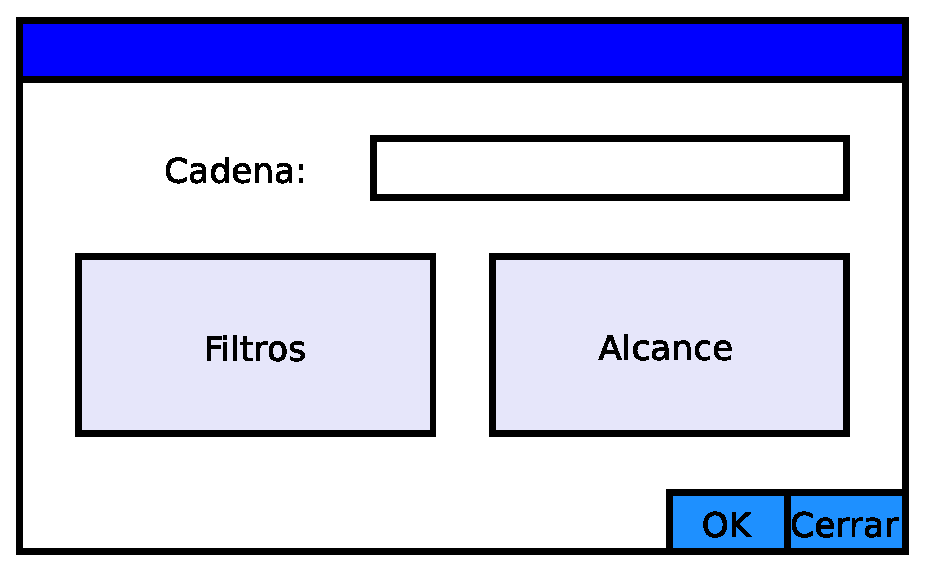
\includegraphics[height=.35\textheight]{desarrollo/prototiposInterfaz/dialogobusqueda}
  \caption{Prototipo del di�logo de b�squeda}
  \label{fig:proto_dlgbusqueda}
\end{figure}

\begin{figure}
  \centering
  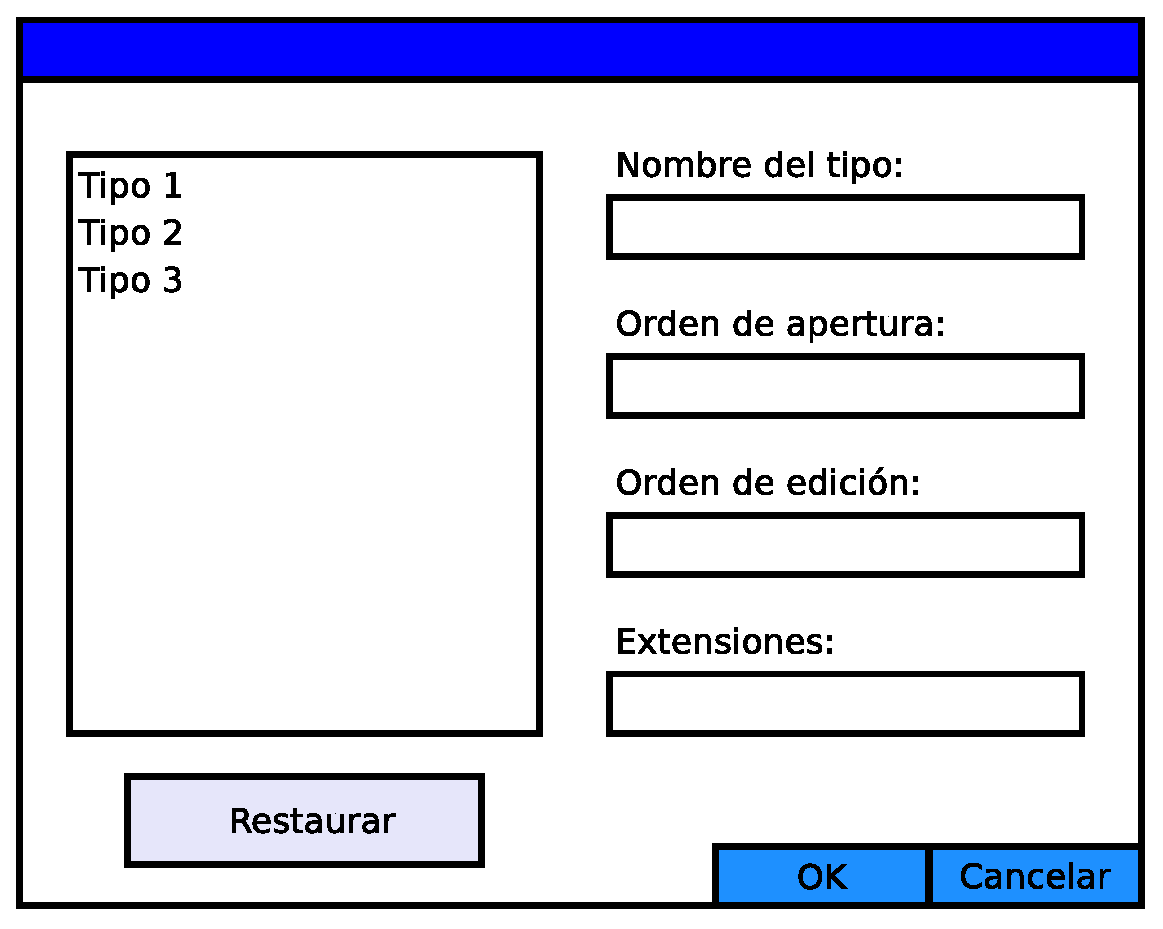
\includegraphics[width=.8\textwidth]{desarrollo/prototiposInterfaz/dialogotipos}
  \caption{Prototipo del di�logo de gesti�n de descriptores de formatos de documentos}
  \label{fig:proto_dlgdfd}
\end{figure}

\begin{figure}
  \centering
  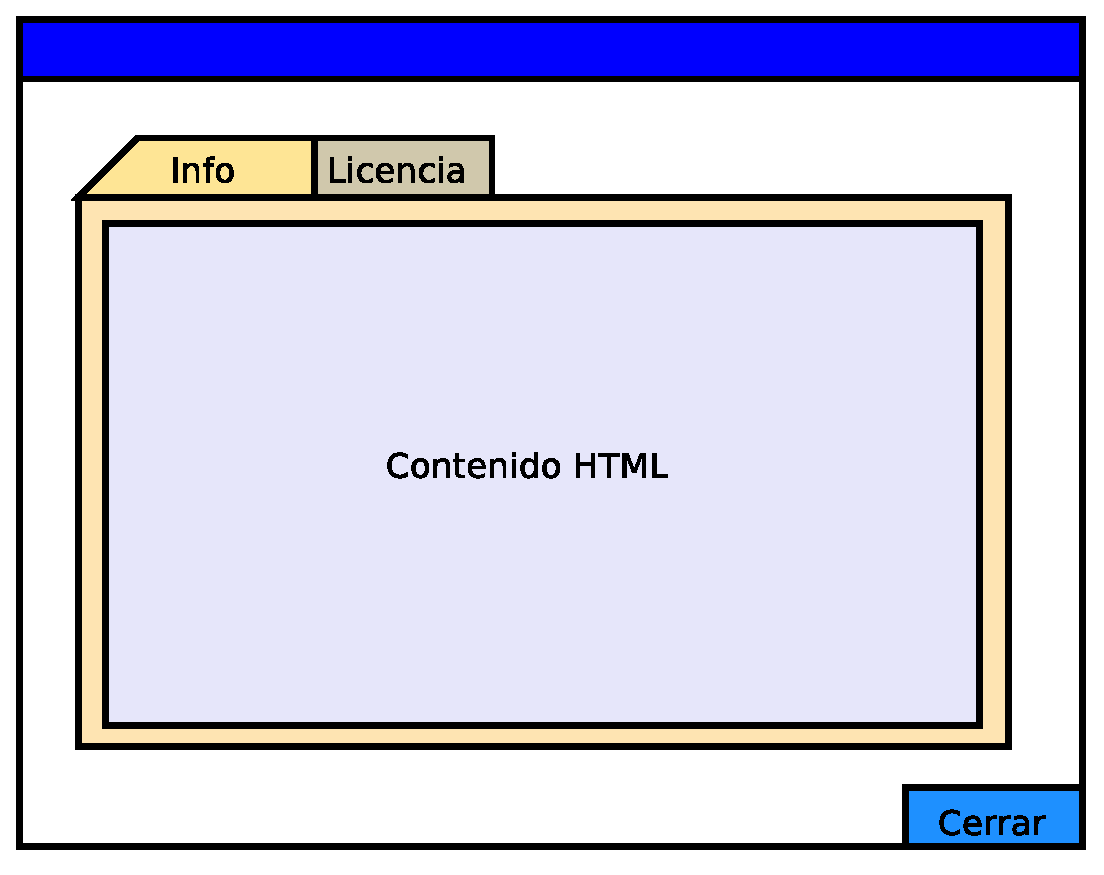
\includegraphics[height=.4\textheight]{desarrollo/prototiposInterfaz/dialogoacercade}
  \caption{Prototipo del di�logo de informaci�n del programa}
  \label{fig:proto_dlgacercade}
\end{figure}

\subsection{Funcionales}
\label{sec:req_func}

\index{requisitos!funcionales}

\begin{itemize}
\item Generar ficheros \ac{XML} que engloben la informaci�n de una
  fuente Lisp, su demostraci�n por \ac{ACL2} asociada y referencias a
  todas las otras fuentes Lisp (libros de \ac{ACL2}) de que dependa.

\item Permitir la visualizaci�n de documentos pertenecientes a
  lenguajes basados en \ac{YAML} 1.1, y la posterior creaci�n de hojas
  espec�ficas a �stos.

\item Navegar por m�ltiples documentos a la vez, abstrayendo al
  usuario si �ste lo desea de los detalles de la estructura de sus
  versiones \ac{XML}.

\item Mantener un historial de documentos recientes, f�cilmente
  accesible por el usuario.

\item Permitir editar los documentos visualizados con el editor
  favorito del usuario para el formato correspondiente, si est�n
  presentes en el sistema. Puede que en ciertos casos s�lo dispongamos
  del \ac{XML} final.

\item Regenerar cualquier documento abierto si se producen cambios en
  �l en alg�n momento, pudiendo mantener el editor y el visor abiertos
  a la vez.

\item Relacionar los elementos del documento entre s�, y con elementos
  espec�ficos de otros documentos.

\item Generar autom�ticamente informaci�n adicional que pueda ser de
  inter�s para el usuario.

\item Realizar b�squedas por el documento, sin p�rdidas de informaci�n
  respecto del texto original, usando diversos filtros y pudiendo
  limitar su alcance.

\item Repetir la �ltima b�squeda realizada.

\item Personalizar las �rdenes usadas para lanzar el editor o el
  conversor de cualquiera de los formatos aceptados, y volver a los
  ajustes por defecto en cualquier momento.

\item Cambiar el tipo y/o formato de la informaci�n mostrada durante
  la ejecuci�n del programa.
\end{itemize}

\subsection{Atributos del sistema software}
\label{sec:req_attr}

\index{requisitos!atributos}

En este proyecto, la mantenibilidad es fundamental para que
posteriores ampliaciones y correcciones se hagan de forma r�pida y
sencilla, dada la complejidad de la herramienta cuyo uso se pretende
facilitar.

Tambi�n ser�a deseable la separaci�n entre la l�gica de visualizaci�n
y el resto del sistema por la posibilidad de que los usuarios (v�ase
\S\ref{sec:desc_usuarios}) extiendan sus capacidades de visualizaci�n
sin tener que modificar el c�digo fuente del proyecto, s�lo
modificando o a�adiendo ficheros de datos. Separar la l�gica de
conversi�n de \visor{} de cuestiones espec�ficas a \postprocesador{}
posibilitar� su uso para formatos distintos a demostraciones de
\ac{ACL2}, y que tampoco tengan por qu� ser basados en \ac{XML}.

La transportabilidad, aunque no imprescindible, se corresponde con el
deseo de permitir un libre uso de este proyecto como una herramienta
m�s para los usuarios de \ac{ACL2} que limite en lo m�nimo posible su
elecci�n de sistema operativo.

Con vistas a ampliar la base de usuarios potencial de \visor{} y sus
extensiones, cobrar� importancia no solo la facilidad de uso, sino
tambi�n la facilidad de instalaci�n, controlando el n�mero de
dependencias externas y, cuando esto no sea posible, reduciendo su
impacto en la complejidad de la instalaci�n.

%%% Local Variables: 
%%% mode: latex
%%% TeX-master: "../memoria"
%%% End: 


\section{An�lisis del sistema}
\label{sec:analisis}
%%
%% analisis.tex
%% Copyright (C) 2008 Antonio Garc�a Dom�nguez
%% $Id: analisis.tex 612 2008-06-25 10:04:09Z antonio $
%%

\subsection{Historias de usuario}
\label{sec:historiasusuario}
%%
%% husuario.tex
%% Copyright (C) 2008 Antonio Garc�a Dom�nguez
%% $Id: husuario.tex 624 2008-07-02 21:40:46Z antonio $
%%

\index{historia de usuario|see{pr�ctica XP!historia de usuario}}

Como ya se coment� en \S\ref{sec:xp_practicas}
(p�gina~\pageref{sec:xp_practicas}), los proyectos basados en \ac{XP}
se estructuran en torno a las historias de los usuarios, que describen
un comportamiento o propiedad deseada del sistema en sus propias
palabras.

Mientras se redactan, el equipo de desarrolladores, tras realizar un
an�lisis superficial del trabajo implicado con ayuda del cliente,
asigna a cada historia un tiempo estimado de finalizaci�n en d�as
ideales y un riesgo. El cliente puede, en funci�n de esos factores y
de sus intereses, marcar la prioridad de una historia.

Una historia de usuario puede ser de muy alto nivel o de muy bajo
nivel, pudiendo unirse varias historias de bajo nivel en una sola, o
dividirse una de alto nivel en varias m�s sencillas.

Pasaremos a listar las historias de usuario que se han ido acumulando
a lo largo de la comunicaci�n con los clientes durante el desarrollo
del PFC, es decir, mis directores de proyecto, usuarios de \ac{ACL2} y
por lo tanto partes interesadas.

En los casos de \postprocesador{} y \yaxml{}, hay varias historias
pospuestas para futuras iteraciones, sin que ello impida entregar una
versi�n funcional (recordemos el principio ``Margen'' de \ac{XP}).

Dividiremos la mayor�a de las historias en tareas, dando estimaciones
iniciales del tiempo necesario para cada una. Otras ser�n lo bastante
concretas como para no necesitar ninguna subdivisi�n.

En esta lista de historias de usuario no se incluyen aquellas que se
completaron durante el Proyecto Fin de Carrera ``Post-procesador y
Visor de Demostraciones del Sistema ACL2''.

\subsubsection{\nombrevisor{}}
\label{sec:husuario_visor}

\begin{enumerate}
\item \label{item:multidoc}
  \begin{quote}
    ``A�adir soporte para visualizar varios ficheros a la vez y
    enlazarlos entre s�.''
  \end{quote}

  Esta historia de usuario es muy corta para todo el trabajo que
  implica:

  \begin{enumerate}
  \item Concentrar el estado de visualizaci�n del documento actual en
    un modelo de presentaci�n, para as� poder cambiar entre los
    estados de cada documento: 3 d�as ideales. Completada.

  \item Integrar de nuevo y depurar toda la funcionalidad de la
    aplicaci�n con este nuevo dise�o: 3 d�as ideales. Completada.

  \item A�adir una interfaz \ac{TDI} a XMLEye, y asegurar su
    integraci�n con el \emph{Look and Feel} instalado: 4 d�as
    ideales. Completada.

  \item A�adir la posibilidad de establecer hiperv�nculos entre varios
    documentos: 2 d�as ideales. Completada.
  \end{enumerate}

\item 
  \begin{quote}
    ``El visor no deber�a saber absolutamente nada de \ac{ACL2}. Nada
    en su interfaz gr�fica ni en su implementaci�n nos debe recordar
    que podemos trabajar con \ac{ACL2}. Pero s� podr�a saber algo de
    un procesador externo que tradujera ficheros de un formato, del
    que el visor tampoco sabe nada, a \ac{XML}. Tambi�n podr�a conocer
    la existencia de hojas de estilo \ac{XSLT} y de herramientas
    externas, como un editor, como de hecho ocurre ahora.''
  \end{quote}

  \begin{enumerate}
  \item Mover toda la l�gica propia de \ac{ACL2} a \postprocesador{},
    y retirarla de \visor{}: 0,5 d�a ideal para retirarla. V�ase la
    historia~\ref{item:integrar-pproc-acl2} de \postprocesador{} para
    la estimaci�n de su recreaci�n. Completada.

  \item Definir la estructura y contenidos de un descriptor de formato
    de documento: 0,5 d�a ideal. Completada.

  \item Implementar y depurar la estructura en 2 niveles del
    repositorio de descriptores, empleando ciertas variables del
    entorno si se hallan definidas: 2 d�as ideales. Completada.

  \item Internacionalizar las cadenas contenidas en los descriptores:
    0,5 d�a ideal. Completada.

  \item Integrar la informaci�n de los descriptores con los controles
    de apertura y edici�n de documentos: 2 d�as ideales. Completada.

  \item Crear un di�logo de gesti�n de los descriptores instalados: 1
    d�a ideal. Completada.
  \end{enumerate}

\item 
  \begin{quote}
    ``Vigilar directamente el fichero fuente en caso de cambios, en vez de
    solamente cuando se cierra el editor. As�, si uno abre el editor, hace
    un par de cambios y guarda (sin cerrar el editor), tambi�n se
    actualizar�. En caso de que se desactive temporalmente la
    reimportaci�n autom�tica, tambi�n deber�a funcionar correctamente si
    en ese intervalo se hicieron cambios.''
  \end{quote}

  Esta historia implica:

  \begin{itemize}
  \item Resolver unas condiciones de carrera conocidas que produc�an
    fallos intermitentes en la reimportaci�n autom�tica. Tiempo
    estimado: 1 d�a ideal. Completada.

  \item Refinar el dise�o del momento para evitar que al reabrir el
    documento, apareciera como una nueva pesta�a. Tiempo estimado: 1
    d�a ideal. Completada.

  \item Implementar la detecci�n y notificaci�n con un hilo pausable
    de baja prioridad en segundo plano, activado de forma
    intermitente. Tiempo estimado: 1 d�a ideal. Completada.
  \end{itemize}

\end{enumerate}

\subsubsection{\nombrepostprocesador{}}
\label{sec:husuario_pproc}

\begin{enumerate}
\item 
  \begin{quote}
    ``Normalizar la estructura de \postprocesador{} para que siga la de
    un m�dulo del CPAN y se porte mejor a la hora de en el futuro
    hacer un paquete Debian.''
  \end{quote}

  Tiempo estimado: 2 d�as ideales. Completada.

\item 
  \begin{quote}
    ``Llevar la cuenta de en qu� paquete (espacio de nombres) estamos
    trabajando. Puede saberse por el indicador (prompt).''
  \end{quote}

  Se requerir�a a�adir el filtrado de la orden \orden{in-package} y
  del indicador de \ac{ACL2}, modificando en consecuencia la salida
  \ac{XML}.

  Tiempo estimado: 1 d�a ideal. Completada.

\item \label{item:hanoi}

  \begin{quote}
    ``Tratar el ejemplo de las Torres de Hanoi de~\cite{Hanoi},
    dividi�ndolo en tres partes: \fichero{books/hanoi.lisp}, libro que
    define el algoritmo para resolver el problema y todo lo necesario
    excepto el propio teorema del n�mero de intercambios;
    \fichero{books/hanoi.acl2}, que se encarga de definir el paquete y
    certificar el libro; y \fichero{hanoi-use.lisp}, que incluye el
    libro y contiene el teorema con el n�mero de intercambios.''
  \end{quote}

  Una vez la capacidad de visualizar y enlazar entre s� varios
  documentos est� a�adida en \visor{} (v�ase su
  historia~\ref{item:multidoc}), habr�a que:

  \begin{itemize}
  \item Crear un m�dulo de detecci�n de dependencias que utilice un
    simple an�lisis superficial de sus �rdenes, de forma recursiva, y
    genere un �ndice de cada libro con los identificadores de los
    eventos que define y los libros de que depende a su vez. Tiempo
    estimado: 3 d�as ideales. Completada.

  \item Implementar el procesamiento de la salida de los eventos
    \orden{include-book}, \orden{certify-book}, \orden{defpkg} e
    \orden{in-package}. Tiempo estimado: 2 d�as ideales. Completada.
  \end{itemize}

\item 

  \begin{quote}
    ``Mejorar los informes de errores de las pruebas de regresi�n,
    evitando que fallen con diferencias insignificantes.''
  \end{quote}

  Requiere:

  \begin{itemize}
  \item Volver a implementar las pruebas de regresi�n, esta vez
    calculando la diferencia entre los documentos no a partir de las
    l�neas de texto que lo componen, sino usando el �rbol DOM
    resultado de analizar los dos documentos \ac{XML}. Tiempo
    estimado: 2 d�as ideales. Completado.

  \item Implementar el c�digo necesario para ignorar aquellas
    diferencias que no sean de inter�s. Tiempo estimado: 1 d�a
    ideal. Completado.
  \end{itemize}

\item \label{item:integrar-pproc-acl2}

  \begin{quote}
    ``Integrar \postprocesador{} con ACL2, haciendo que
    autom�ticamente genere las salidas y las sit�e en ficheros
    \fichero{.out} y \fichero{.xml} en el mismo directorio, realizando
    una gesti�n de dependencias al estilo GNU Make entre ellos y la
    fuente Lisp. As� evitar�amos importar varias veces el mismo
    fichero, y se podr�a simplificar el visor.''
  \end{quote}

  Una vez est� terminada la tarea~\ref{item:hanoi}, habr�a que
  modificar el c�digo que recibe el texto de la demostraci�n de
  \ac{ACL2} y lanza el proceso de an�lisis para que invoque �l mismo a
  \ac{ACL2} en caso de que el fichero \fichero{.xml} no exista o se
  halle desactualizado respecto a la fuente Lisp.

  Tiempo estimado: 1 d�a ideal. Completada.

\item 

  \begin{quote}
    ``Manejar los eventos definidos por el usuario con
    \orden{make-event} y las expansiones de macros creadas con
    \orden{defmacro}.''
  \end{quote}

  No est� del todo clara la forma de resolver esta historia de
  usuario. Un an�lisis superficial sugiere esta divisi�n en tareas:

  \begin{itemize}
  \item Instrumentar el c�digo Lisp con llamadas previas a
    \verb#:trans1# sobre la orden desconocida, sin que se produzcan
    modificaciones en el espaciado de cualquiera del resto de las
    l�neas del documento. Tiempo estimado: 2 d�as ideales. Pospuesta.

  \item Usar la orden resultante de \verb#:trans1# como el enunciado
    de la orden para la siguiente salida. Tiempo estimado: 2 d�as
    ideales, por posibles cambios importantes a realizar en el
    dise�o. Pospuesta.

  \item Registrar de alguna forma la expansi�n producida por
    \orden{make-event}, tomando como base el fichero fuente
    \fichero{basic.lisp} del libro \fichero{make-event} incluido en la
    distribuci�n de \ac{ACL2}. Tiempo estimado: 3 d�as
    ideales. Pospuesta.
  \end{itemize}

\item 

  \begin{quote}
    ``Tratar el caso en que un \orden{include-book} aparezca dentro de un
    \orden{local} (y entonces lo que se incluye es local al libro, no se ve
    fuera). Y esto puede aparecer dentro de un \orden{encapsulate}''.
  \end{quote}

  Hay que refinar la sintaxis de los grafos de dependencias para
  incluir menciones al �mbito de validez de cada entrada: puede que
  dentro de un \orden{encapsulate} se haga referencia a un evento
  \evento{P::F}, y en el nivel global u otro \orden{local} o
  \orden{encapsulate}, se dependa de otro evento distinto con el mismo
  nombre. Limitando el alcance de las definiciones se podr�a tratar
  este problema.

  Tiempo estimado: 3 d�as ideales. Pospuesta.

\item 

  \begin{quote}
    ``Tratar las \emph{forcing rounds}, demostraciones realizadas tras
    la demostraci�n principal sobre cualquier hip�tesis cuya
    aplicaci�n se hubiera forzado durante la demostraci�n anterior (la
    demostraci�n inicial, u otra \emph{forcing round}).''
  \end{quote}
  
  Hay que refinar la divisi�n jer�rquica de las metas y procesar la
  salida espec�fica a las \emph{forcing rounds} estableciendo los
  enlaces correspondientes.

  Tiempo estimado: 3 d�as ideales. Pospuesta.

\item
  \begin{quote}
    ``Tratar todas las opciones que pueden acompa�ar a un \orden{defthm} y a
    un \orden{defun}.''
  \end{quote}

  En el caso de \orden{defthm}, se han de tratar \orden{:rule-classes},
  \orden{:instructions}, \orden{:hints}, \orden{:otf-flg} y
  \orden{:doc}.

  Para \orden{defun}, se han de tratar las declaraciones y la cadena
  de documentaci�n (del estilo del argumento de \orden{:doc}).

  Esta historia se habr�a de dividir entonces en varias tareas
  independientes:
  \begin{enumerate}
  \item Soporte para cadenas de documentaci�n, \orden{:rule-classes} y
    \orden{:otf-flg}: 2 d�as ideales. Completada parcialmente.
  \item Soporte de \orden{:instructions}: 2 d�as ideales. Pospuesta.
  \item Soporte de \orden{:hints}: 2 d�as ideales. Pospuesta.
  \item Soporte de declaraciones (incluye \orden{:hints} e
    \orden{:instructions}): 2 d�as ideales. Pospuesta.
  \end{enumerate}

\item
  \begin{quote}
    ``Marcar las salidas de los nuevos apuntes de
    Moore~\cite{recindacl2}, \emph{Recursion and Induction}.''
  \end{quote}

  El trabajo necesario para implementar esta historia de usuario es
  extensivo, requiriendo implementar todas las historias anteriormente
  propuestas, y a�adir la capacidad a \postprocesador{} de tratar
  macros Lisp.  

  Tiempo estimado: 6 d�as ideales. Pospuesta.

\end{enumerate}

\subsubsection{\nombreyaxml{}}
\label{sec:husuario_yaxml}

\begin{enumerate}
\item 
  \begin{quote}
    ``Abrir documentos \ac{YAML} en \nombrevisor{} sin que suponga una
    p�rdida o alteraci�n de la informaci�n disponible.''
  \end{quote}

  \begin{itemize}
  \item Seleccionar un m�dulo Perl que permita cargar documentos
    \ac{YAML}. Idealmente, deber�a ser Perl puro, pero la velocidad de
    carga y la fiabilidad son m�s importantes. Tiempo estimado: 0,5 d�a
    ideal. Completada.

  \item Definir un primer prototipo del m�dulo que verifique la
    viabilidad del enfoque usado con algunos ejemplos sencillos: 0,5
    d�a ideal. Completada.

  \item Convertir el prototipo en un m�dulo completo al estilo del
    \ac{CPAN}, con pruebas de unidad basadas en Perl que verifiquen la
    conservaci�n de la informaci�n: 1 d�a ideal. Completada.
  \end{itemize}

\item 
  \begin{quote}
    ``Procesar el ejemplo de la factura de la web~\cite{YAXML} de \ac{YAXML}.''
  \end{quote}

  Hay que establecer un mecanismo para detectar la existencia de
  anclas y alias en la estructura de datos generada en memoria,
  evitando tener que volver a analizar el c�digo fuente
  \ac{YAML}. Podr�an buscarse referencias duplicadas, por
  ejemplo. Tiempo estimado: 1 d�a ideal. Completada.

\item 
  \begin{quote}
    ``Preparar hojas de estilos para los marcadores de Firefox y
    volcados del entorno de desarrollo web Django.''
  \end{quote}

  \begin{itemize}
  \item Comprobar que la biblioteca usada analiza correctamente
    documentos del subconjunto \ac{JSON} de \ac{YAML} 1.1 que emplean
    los volcados de Django y los marcadores de Firefox, y en caso
    contrario reemplazar la existente. Tiempo estimado: 1 d�a ideal. Completada.

  \item Comprobar que se procesan debidamente documentos codificados
    en \acs{UTF}-8 con caracteres fuera del conjunto \acs{ASCII} de 7
    bits. Tiempo estimado: 1 d�a ideal. Completada.

  \item Implementar hojas de estilos especializadas para los
    marcadores de Firefox y volcados de Django. Tiempo estimado: 2
    d�as ideales. Pospuesta.
  \end{itemize}

\end{enumerate}

%%% Local Variables: 
%%% mode: latex
%%% TeX-master: "../../memoria"
%%% End: 


\subsection{Casos de uso}
\label{sec:casosuso}
%%
%% Casos de uso de XMLEye
%% Copyright (C) 2008 Antonio Garc�a Dom�nguez
%% $Id: casosuso.tex 629 2008-07-06 13:47:58Z antonio $
%%
\index{meta de usuario|see{casos de uso!meta de usuario}}
\index{subfunci�n|see{casos de uso!subfunci�n}}
\index{casos de uso!meta de usuario}
\index{casos de uso!subfunci�n}

Estos casos de uso nos permiten analizar de manera general y abstracta
qu� es lo que se requiere en conjunto de las historias de usuario de
\visor{} de este Proyecto y la versi�n del Proyecto Fin de Carrera
sobre el que se basa. El diagrama que ilustra las relaciones entre los
distintos casos de uso que cumplen las metas del usuario se puede
hallar en la figura~\ref{fig:diag_casosdeuso}.

El l�mite del sistema establecido engloba �nicamente a \visor{}. Los
conversores externos, entre los cuales se hallan \postprocesador{} y
\visor{}, participan �nicamente como un agente externo. El m�todo de
comunicaci�n con \visor{} se aclarar� m�s tarde, en la fase de
dise�o. A menos que se indique lo contrario, los casos de uso aqu�
mostrados son en general de nivel de meta de usuario.

\begin{figure}
  \centering
  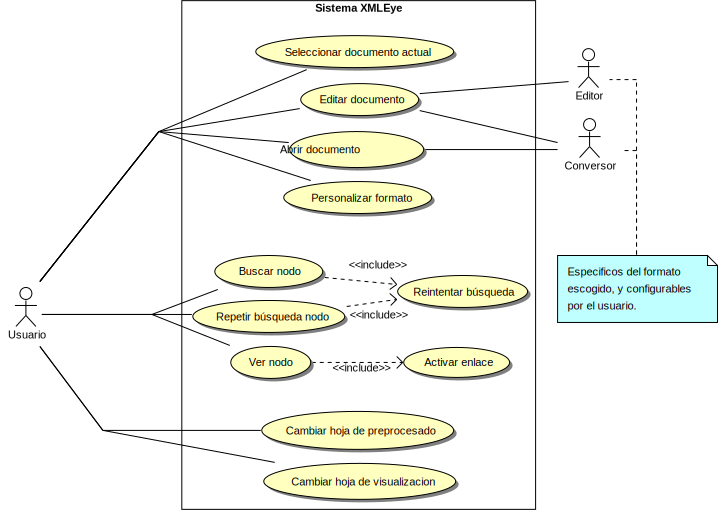
\includegraphics[width=\textwidth]{desarrollo/analisis/casosuso}
  \caption{Diagrama de casos de uso}
  \label{fig:diag_casosdeuso}
\end{figure}

\subsubsection{Seleccionar documento actual}
\label{sec:seleccionar_doc_actual}

\begin{description}
\item[Actor principal] Usuario: desea seleccionar el documento sobre
  el que actuar en el resto de casos de prueba de entre los documentos
  abiertos.
\item[Precondiciones] Existe al menos un documento abierto.
\item[Postcondiciones] Se muestra el documento seleccionado.

\item[Escenario principal] \mbox{}
  \begin{enumerate}
  \item El usuario indica su intenci�n de cambiar de documento.
  \item El sistema proporciona una lista de los documentos disponibles.
  \item El usuario selecciona el documento de la lista. \label{item:select_doc}
  \item El sistema registra la selecci�n, guarda el estado actual de
    la visualizaci�n actual y restaura el estado de la visualizaci�n
    del documento seleccionado, mostr�ndolo tal y como estaba antes de
    haber seleccionado otro documento.
  \end{enumerate}

\item[Variaciones] \mbox{}

  \begin{enumerate}[{\ref{item:select_doc}}a.]
  \item El documento es el mismo que el actual:
    \begin{enumerate}[1.]
    \item El sistema cancela el cambio de uso.      
    \end{enumerate}
  \end{enumerate}

\end{description}

\subsubsection{Editar documento}
\label{sec:casouso_editar}

\begin{description}
\item[Actor principal] Usuario: desea editar en paralelo a la
  visualizaci�n el enunciado fuente del documento actual de forma r�pida
  y sencilla usando su editor preferido.
\item[Actores secundarios] \mbox{}
  \begin{description}
  \item[Editor] Editor preferido del usuario para el formato del
    documento actual.
  \item[Conversor] Sistema externo ocupado de convertir el documento a
    \ac{XML}, si es necesario.
  \end{description}
\item[Precondiciones] Existe un documento abierto.
\item[Postcondiciones] Se ha abierto el documento con el editor
  especificado en el descriptor de formato correspondiente.
\item[Escenario principal] \mbox{}
  \begin{enumerate}
  \item El usuario indica su intenci�n de editar el enunciado del
    documento abierto.
  \item El sistema lanza el editor, y contin�a con su funcionamiento
    normal, esperando en segundo plano a que se realicen cambios.
    \label{item:edit_espera}
  \item El usuario guarda algunos cambios en el documento.
  \item El sistema detecta los cambios: se regenera la visualizaci�n
    completa del documento.
  \item El sistema pasa de nuevo a la espera de m�s cambios en segundo
    plano.
  \end{enumerate}

\item[Variaciones] \mbox{}

  \begin{enumerate}[{\ref{item:edit_espera}}a.]
  \item La invocaci�n del editor ha fallado:
    \begin{enumerate}[1.]
    \item El sistema indica el error y cancela el caso de uso.
    \end{enumerate}

  \item Se ha cerrado el documento:
    \begin{enumerate}[1.]
    \item El sistema deja de monitorizar el documento.
    \end{enumerate}
  \end{enumerate}

\end{description}

\subsubsection{Abrir documento}
\label{sec:casouso_abrir}

\begin{description}
\item[Actor principal] Usuario: desea examinar la versi�n m�s reciente
  del documento en general, para despu�s centrarse en los nodos de su
  inter�s.
\item[Actores secundarios] Conversor: sistema externo que se ocupa de
  convertir el documento proporcionado a \ac{XML}.
\item[Precondiciones] Ninguna.
\item[Postcondiciones] Se carga la versi�n m�s reciente del documento
  elegido por el usuario.
\item[Escenario principal]\mbox{}
  \begin{enumerate}
  \item El usuario indica su intenci�n de abrir un documento ya
    existente.
  \item El sistema muestra los documentos disponibles.
  \item El usuario selecciona un
    documento. \label{item:abrir_cancelar}
  \item El sistema comprueba que el documento
    existe. \label{item:abrir_docexiste}
  \item El sistema le asocia el primer formato con una extensi�n
    coincidente, y aplica su conversor, si tiene uno asociado, al
    documento. \label{item:abrir_asociar_formato}.
  \item El sistema muestra el documento elegido, tras a�adirlo a la
    lista de documentos abiertos.
  \end{enumerate}
\item[Variaciones]\mbox{}

  \begin{enumerate}[{\ref{item:abrir_cancelar}}a.]
  \item El usuario cancela la selecci�n de documento:
    \begin{enumerate}[1.]
    \item El sistema cancela el caso de uso.
    \end{enumerate}
  \end{enumerate}

  \begin{enumerate}[{\ref{item:abrir_docexiste}}a.]
  \item El documento no existe:
    \begin{enumerate}[1.]
    \item El sistema muestra el error y cancela el caso de uso.
    \end{enumerate}
  \end{enumerate}

  \begin{enumerate}[{\ref{item:abrir_asociar_formato}}a.]
  \item No existe un formato con una extensi�n coincidente:
    \begin{enumerate}[1.]
    \item El sistema utiliza el formato por defecto, \ac{XML}, que no
      tiene un conversor asociado.
    \end{enumerate}
  \end{enumerate}
\end{description}

\subsubsection{Personalizar formato}
\label{sec:personalizar_formato}

\begin{description}
\item[Actor principal] Usuario: desea cambiar las opciones de alguno
  de los formatos instalados.

\item[Precondiciones] Existe al menos un formato instalado en el
  sistema.

\item[Postcondiciones] Se cambian los ajustes locales del usuario para
  el formato indicado, sin cambiar los ajustes globales.

\item[Escenario principal] \mbox{}
  \begin{enumerate}
  \item El usuario indica su intenci�n de cambiar las opciones de alguno de
    los formatos.

  \item El sistema muestra la lista de los formatos disponibles. \label{item:pers_primero}

  \item El usuario selecciona un formato de la lista.

  \item El sistema muestra los campos modificables del formato:

    \begin{itemize}
    \item La traducci�n del nombre del formato que se ajuste mejor a
      la localizaci�n activa por defecto en el entorno del usuario.
    \item La orden usada para invocar al editor preferido del usuario
      para dicho formato.
    \item La orden usada para invocar al conversor a \ac{XML}
      preferido del usuario para dicho formato.
    \item La lista de extensiones, separadas por comas, con las que se
      asociar� a este formato.
    \end{itemize}
    
  \item El usuario modifica el valor de los campos. 

  \item El sistema solicita confirmaci�n al usuario.

  \item El usuario proporciona la confirmaci�n. \label{item:pers_conf}

  \item El sistema registra los cambios a nivel del usuario actual,
    sin modificar los ajustes globales, y los hace efectivos a partir
    del mismo momento.
  \end{enumerate}

\item[Variaciones] \mbox{}

  \begin{enumerate}[{\ref{item:pers_primero}-\ref{item:pers_conf}}a.]
  \item El usuario cancela la personalizaci�n:
    \begin{enumerate}[1.]
    \item El sistema cancela el caso de uso, sin que se hagan
      efectivos los campos.
    \end{enumerate}
  \end{enumerate}

  \begin{enumerate}[{\ref{item:pers_conf}}a.]
  \item Los campos de nombre del formato, orden de edici�n o
    extensiones se hallan vac�os o s�lo contienen espacios en blanco,
    alguna de las extensiones pasadas contiene espacios o est� vac�a,
    o la orden de importaci�n contiene solamente uno o m�s espacios en
    blanco:
    \begin{enumerate}[1.]
    \item El sistema informa de la situaci�n y solicita corregir dicha
      situaci�n.
    \end{enumerate}
  \end{enumerate}

\end{description}

\subsubsection{Buscar nodo}
\label{sec:casouso_buscarnodo}

\begin{description}
\item[Actor principal] Usuario: desea localizar r�pidamente los nodos
  que cumplan una serie de condiciones.
\item[Precondiciones] Hay un documento abierto.
\item[Postcondiciones] Se muestra el resultado de la b�squeda.
\item[Escenario principal] \mbox{}
  \begin{enumerate}
  \item El usuario indica su intenci�n de iniciar una nueva b�squeda.
    \label{item:buscar_inicio}
  \item El sistema solicita la clave de b�squeda.
  \item El usuario introduce la clave de b�squeda.
  \item El sistema comprueba que la clave de b�squeda es v�lida.
    \label{item:buscar_chkclave}
  \item El sistema presenta al usuario las opciones de filtrado.
  \item El usuario elige las opciones de filtrado.
    \label{item:buscar_filtro}
  \item El sistema realiza la b�squeda a partir del nodo actual y
    muestra el primer resultado. \label{item:buscar_res}
  \end{enumerate}
\item[Variaciones] \mbox{}
  
  \begin{enumerate}[{\ref{item:buscar_inicio}-\ref{item:buscar_filtro}}a.]
  \item El usuario cancela la b�squeda:
    \begin{enumerate}[1.]
    \item El sistema cancela el caso de uso.
    \end{enumerate}
  \end{enumerate}
  
  \begin{enumerate}[{\ref{item:buscar_chkclave}}a.]
  \item La clave no es v�lida:
    \begin{enumerate}[1.]
    \item El sistema indica el error y pide una nueva clave.
    \end{enumerate}
  \end{enumerate}
  
  \begin{enumerate}[{\ref{item:buscar_res}}a.]
  \item No hay resultados:
    \begin{enumerate}[1.]
    \item \emph{include(Reintentar b�squeda)}
    \end{enumerate}
  \end{enumerate}
\end{description}

\subsubsection{Repetir b�squeda}
\label{sec:casouso_repbusqueda}

\begin{description}
\item[Actor principal] Usuario: desea encontrar otro nodo que cumpla
  las mismas condiciones que el anterior, sin tener que volver a
  especificar las opciones de filtrado.
\item[Precondiciones] Hay un documento abierto.
\item[Postcondiciones] Se muestra el siguiente nodo que cumple las
  condiciones de la �ltima b�squeda.
\item[Escenario principal] \mbox{}

  \begin{enumerate}
  \item El usuario desea repetir la b�squeda anterior:
  \item El sistema comprueba que existe una b�squeda anterior.
    \label{item:chk_busqanterior}
  \item El sistema realiza de nuevo la b�squeda a partir del nodo
    actual y muestra el primer resultado.
    \label{item:repetirbusq_buscar_res}
  \end{enumerate}

\item[Variaciones] \mbox{}

  \begin{enumerate}[{\ref{item:chk_busqanterior}}a.]
  \item No existen b�squedas anteriores:
    \begin{enumerate}[1.]
    \item El sistema indica el error y cancela el caso de uso.
    \end{enumerate}
  \end{enumerate}
  
  \begin{enumerate}[{\ref{item:repetirbusq_buscar_res}}a.]
  \item No hay resultados:
    \begin{enumerate}[1.]
    \item \emph{include(Reintentar b�squeda)}
    \end{enumerate}
  \end{enumerate}
\end{description}

\subsubsection{Reintentar b�squeda}
\label{sec:casouso_reintentar_busq}

\begin{description}
\item[Actor principal] Usuario: desea visualizar un nodo que cumpla
  las condiciones, aunque tenga que relajar el alcance de la b�squeda.
\item[Nivel de caso de uso] Subfunci�n.
\item[Precondiciones] Hay un documento abierto.
\item[Postcondiciones] Se muestra el primer nodo que cumple las nuevas
  condiciones relajadas.
\item[Escenario principal] \mbox{}
  \begin{enumerate}
  \item El sistema indica la situaci�n y ofrece repetir la b�squeda
    con par�metros m�s generales.
  \item El usuario acepta. \label{item:buscar_res_aceptar}
  \item El sistema relanza la b�squeda y muestra el primer
    resultado. \label{item:buscar_res_repetir}
  \end{enumerate}

\item[Variaciones] \mbox{}
  \begin{enumerate}[{\ref{item:buscar_res_aceptar}}a.]
  \item El usuario rechaza la oferta: 
    \begin{enumerate}[1.]
    \item El sistema cancela el caso de uso.
    \end{enumerate}
  \end{enumerate}

  \begin{enumerate}[{\ref{item:buscar_res_repetir}}a.]
  \item No hay resultados:
    \begin{enumerate}[1.]
    \item El sistema indica la situaci�n y cancela el caso de uso.
    \end{enumerate}
  \end{enumerate}
\end{description}

\subsubsection{Ver nodo}
\label{sec:casouso_selnodo}

\begin{description}
\item[Actor principal] Usuario: desea visualizar la informaci�n acerca
  de un nodo del documento.
\item[Precondiciones] Hay un documento abierto.
\item[Postcondiciones] Se muestra la informaci�n del nodo seleccionado.
\item[Escenario principal] \mbox{}
  \begin{enumerate}
  \item El usuario indica el nodo del documento que desea ver.
  \item El sistema comprueba que existe. \label{item:selnode_chknode}
  \item El sistema muestra la informaci�n del nodo al usuario, dejando
    que interact�e con �l. \label{item:selnode_interact}
  \end{enumerate}
\item[Variaciones] \mbox{}

  \begin{enumerate}[{\ref{item:selnode_chknode}}a.]
  \item El nodo no existe:
    \begin{enumerate}[1.]
    \item El sistema muestra una visualizaci�n vac�a.
    \end{enumerate}
  \end{enumerate}

  \begin{enumerate}[{\ref{item:selnode_interact}}a.]
  \item El usuario activa uno de los hiperv�nculos disponibles:
    \begin{enumerate}[1.]
    \item \emph{include(Activar enlace)}
    \end{enumerate}
  \end{enumerate}

\end{description}

\subsubsection{Activar enlace}
\label{sec:casouso_activar_enlace}

\begin{description}
\item[Actor principal] Usuario: desea visualizar el recurso al que
  se�ala el enlace activado.
\item[Nivel de caso de uso] Subfunci�n.
\item[Precondiciones] Hay un documento abierto, y se est� visualizando
  un nodo.
\item[Postcondiciones] Se muestra el destino del enlace pulsado, si
  tiene uno definido.
\item[Escenario principal] \mbox{}
  \begin{enumerate}
  \item El usuario activa el enlace en cuesti�n de la visualizaci�n
    del nodo actual.

  \item Si el enlace se�ala a otro nodo, se ejecuta el caso de uso
    ``Ver nodo'' sobre �l, y se termina el caso de uso.

  \item Si el enlace se�ala a una \ac{URL}, se muestra el documento en
    uno de los navegadores Web disponibles, y se termina el caso de uso.

  \item Si el enlace se�ala a un ancla de la visualizaci�n \ac{HTML}
    del nodo actual, se desplaza la posici�n actual a la del ancla, y
    se termina el caso de uso.

  \item Si el enlace se�ala a un nodo de otro documento, se visualiza
    dicho documento mediante ``Visualizar documento'', posteriormente
    se ejecuta ``Ver nodo'' sobre el nodo especificado, y se termina
    el caso de uso.

  \item El sistema cancela el caso de uso.
  \end{enumerate}

\end{description}

\subsubsection{Cambiar hoja de preprocesado}
\label{sec:casouso_hoja_preproc}

\begin{description}
\item[Actor principal] Usuario: desea cambiar la forma en
  que se muestra la estructura del documento.

\item[Precondiciones] Existe al menos un documento abierto y
  seleccionado.

\item[Postcondiciones] Se le muestra al usuario la nueva estructura
  del documento, procesada desde el texto \ac{XML} original a trav�s
  de la hoja seleccionada. Se usar� esta hoja para todos los ficheros
  que se abran a continuaci�n.

\item[Escenario principal] \mbox{}
  \begin{enumerate}
  \item El usuario indica su intenci�n de cambiar la hoja
    de preprocesado en uso. \label{item:cambio_hoja_inicio}
  \item El sistema muestra una lista de las hojas de preprocesado
    disponibles.
  \item El usuario selecciona una hoja de la
    lista. \label{item:cambio_hoja_selecc}
  \item El sistema recupera el texto \ac{XML} original del documento y
    lo procesa mediante la nueva hoja seleccionada.
  \item El sistema muestra la nueva estructura del documento, y vac�a
    la visualizaci�n del nodo actual, al no haber ninguno
    seleccionado.
  \item El sistema registra la hoja seleccionada como hoja de
    preprocesado por defecto para todos los documentos abiertos en
    adelante.
  \end{enumerate}

\item[Variaciones] \mbox{}

  \begin{enumerate}[{\ref{item:cambio_hoja_inicio}-\ref{item:cambio_hoja_selecc}}a.]
  \item El usuario cancela la selecci�n:
    \begin{enumerate}[1.]
    \item El sistema cancela la ejecuci�n del caso de uso.
    \end{enumerate}
  \end{enumerate}

\end{description}

\subsubsection{Cambiar hoja de visualizaci�n}
\label{sec:casouso_hoja_visualizacion}

\begin{description}
\item[Actor principal] Usuario: desea cambiar la forma en que se
  muestra la informaci�n de los nodos de un documento.

\item[Precondiciones] Existe al menos un documento abierto y
  seleccionado.

\item[Postcondiciones] Se visualiza el nodo actual y todos los
  posteriormente seleccionados en el documento actual y en todos los
  documentos abiertos posteriormente bajo la nueva hoja.

\item[Escenario principal] \mbox{}
  \begin{enumerate}
  \item El usuario indica su intenci�n de cambiar la hoja de
    visualizaci�n para el documento actual. \label{item:cambio_hoja_v_inicio}
  \item El sistema muestra la lista de las hojas de visualizaci�n
    disponibles.
  \item El usuario selecciona una de las hojas de la
    lista. \label{item:cambio_hoja_v_selecc}
  \item El sistema actualiza la visualizaci�n del nodo actualmente
    seleccionado, si lo hay.
  \item El sistema registra la hoja seleccionada como hoja de
    visualizaci�n por defecto para los documentos abiertos de ahora en
    adelante.
  \end{enumerate}
\item[Variaciones] \mbox{}

  \begin{enumerate}[{\ref{item:cambio_hoja_v_inicio}-\ref{item:cambio_hoja_v_selecc}}a.]
  \item El usuario cancela la selecci�n:
    \begin{enumerate}[1.]
    \item El sistema cancela la ejecuci�n del caso de uso.
    \end{enumerate}
  \end{enumerate}

\end{description}

%%% Local Variables: 
%%% mode: latex
%%% TeX-master: "../../memoria"
%%% End: 


\subsection{Modelo conceptual de datos del dominio de \acs{ACL2}}
\label{sec:datos_conceptual_acl2}
%%
%% datosconceptual.tex
%% $Id: datosconceptual_acl2.tex 617 2008-06-28 17:00:10Z antonio $ 
%%

\subsubsection{Notaci�n}
\label{sec:conceptual_notacion}

Se ha usado \ac{UML} 2.0, con las siguientes modificaciones:
\begin{itemize}
\item Por claridad, algunas clases se hallan duplicadas en los
  diagramas. Para evitar confusiones, las duplicaciones ocultan los
  atributos y se hallan en color azul.
\item Igualmente, se han omitido las multiplicidades unitarias en las
  asociaciones y composiciones.
\end{itemize}

\subsubsection{Descripci�n general}
\label{sec:conceptual_acl2_general}

Para \postprocesador{}, los conceptos a tratar son entes abstractos
relacionados con el proceso de demostraci�n de \ac{ACL2}.

As�, partimos de un \clase{Enunciado}, colecci�n de \clase{Orden}es de
\ac{ACL2} que produce una \clase{Demostraci�n}. Esta
\clase{Demostraci�n} asocia a cada \clase{Orden} un \clase{Resultado}
con la salida obtenida de \ac{ACL2}. Esta contendr� diversos tipos de
informaci�n seg�n la \clase{Orden} usada.

Puede que nuestro \clase{Enunciado} sea la ra�z de un proyecto de
\ac{ACL2}, y se halle definido en base a una serie de definiciones ya
demostradas en \clase{Libro}s existentes. Es importante ver que un
\clase{Libro} puede requerir de una serie de definiciones previas a su
vez: seg�n la terminolog�a de \ac{ACL2}, ser�a su \emph{mundo
  inicial}. Todo \clase{Evento} pertenece a un \clase{Paquete}: si no
se indica su nombre previamente con una orden \orden{in-package}, ser�
``ACL2''.

Adicionalmente, pueden aparecer avisos, errores y observaciones de
\ac{ACL2} al inicio del resultado de la ejecuci�n de una \clase{Orden}
dada.

A su vez, cada \clase{Resultado}, en caso de necesitar demostrar
alguna S-expresi�n, usar� una \clase{Meta} principal, que se podr�
dividir recursivamente en submetas. Cada \clase{Meta} usa un
determinado \clase{Proceso} de demostraci�n.

Se ha dividido el diagrama de clases conceptuales en tres:
\begin{enumerate}
\item Visi�n general del dominio del problema:
  figura~\ref{fig:conceptual_general} de la
  p�gina~\pageref{fig:conceptual_general}.

\item Tipos de Orden: figura~\ref{fig:conceptual_ordenes} de la
  p�gina~\pageref{fig:conceptual_ordenes}.

  Es interesante ver c�mo algunas �rdenes utilizan a otras. Por
  ejemplo, como paso de verificaci�n tras la certificaci�n de un libro
  con \orden{certify-book}, se intentan cargar sus contenidos en el
  mundo de \ac{ACL2}, justo como si se hubiera ejecutado una orden
  \orden{include-book}.

\item Tipos de Proceso: figura~\ref{fig:conceptual_procesos} de la
  p�gina~\pageref{fig:conceptual_procesos}.

\end{enumerate}

\begin{sidewaysfigure}
  \centering
  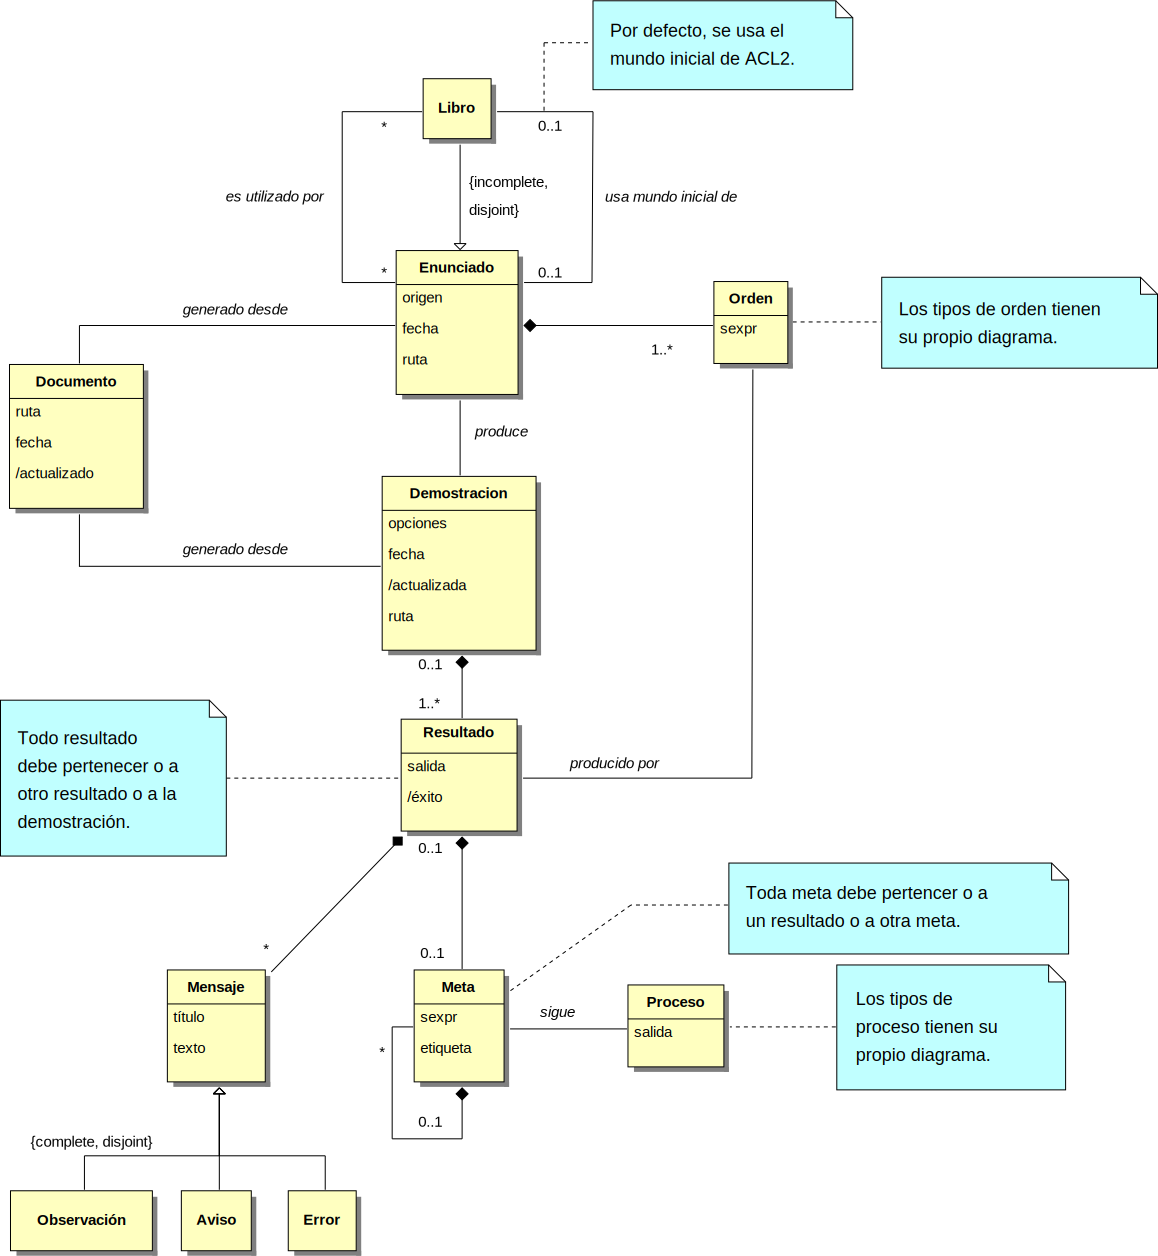
\includegraphics[height=.7\textheight]{desarrollo/analisis/modacl2_general}
  \caption{Diagrama de clases conceptuales general de \acs{ACL2}}
  \label{fig:conceptual_general}
\end{sidewaysfigure}

\begin{sidewaysfigure}
  \centering
  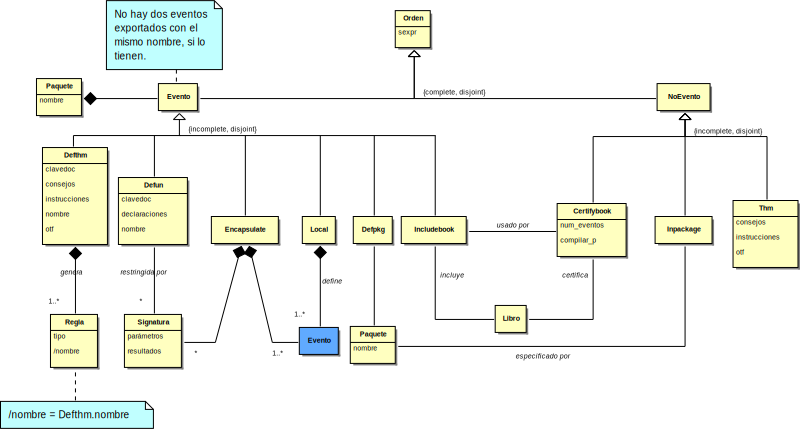
\includegraphics[width=\textwidth]{desarrollo/analisis/modacl2_ordenes}
  \caption{Diagrama de clases conceptuales de �rdenes de \acs{ACL2}}
  \label{fig:conceptual_ordenes}
\end{sidewaysfigure}

\begin{sidewaysfigure}
  \centering
  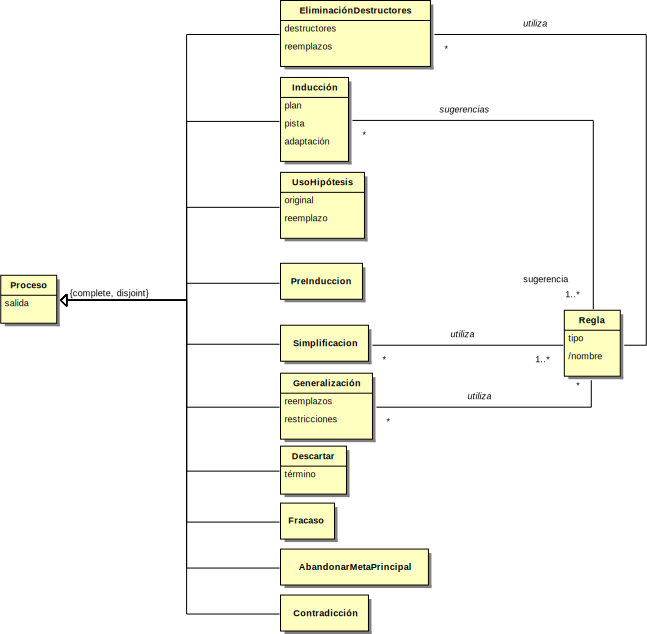
\includegraphics[height=.7\textheight]{desarrollo/analisis/modacl2_procesos}
  \caption{Diagrama de clases conceptuales de procesos de \acs{ACL2}}
  \label{fig:conceptual_procesos}
\end{sidewaysfigure}

\subsubsection{Restricciones textuales}

\begin{enumerate}
\item \emph{Clave externa}: ``nombre'' de \clase{Documento}.
\item \emph{Clave externa}: ``nombre'' de \clase{Paquete}.
\item \emph{Clave externa}: ``nombre'' de cualquier descendiente de
  \clase{Evento}, si lo tiene.
\item \emph{Clave externa}: ``clavedoc'' de cualquier descendiente de
  \clase{Evento}, si la tiene y est� especificada.
\item Todo \clase{Resultado} pertenece o a otro \clase{Resultado} o a una
  \clase{Demostraci�n}.
\item Todo \clase{Meta} pertenece o a otra \clase{Meta} o a un \clase{Resultado}.
\item Toda \clase{Meta} tiene una etiqueta �nica dentro de una \clase{Demostraci�n}.
\item \clase{Resultado}.�xito $\in{} \left\{ \text{verdadero},
    \text{falso} \right\}$.
\item \clase{Documento}.actualizado $\in{} \left\{ \text{verdadero},
    \text{falso} \right\}$.
\item \clase{Demostraci�n}.actualizada $\in{} \left\{ \text{verdadero},
    \text{falso} \right\}$.
\end{enumerate}

\subsubsection{Derivaciones}

\begin{enumerate}
\item \clase{Demostraci�n}.actualizada = ``verdadero'' si
  \clase{Demostraci�n}.fecha es una fecha y hora posterior a
  \clase{Enunciado}.fecha. ``falso'' de lo contrario.
\item \clase{Documento}.actualizado = ``verdadero'' si
  \clase{Demostraci�n}.actualizada y \clase{Documento}.fecha es una
  fecha y hora posterior a \clase{Demostraci�n}.fecha. ``falso'' de lo
  contrario.
\item \clase{Resultado}.�xito = no contiene \clase{Meta} con el
  \clase{Proceso} \clase{Fracaso} y sus \clase{Resultados} de inferior
  nivel (si los hay) tienen �xito.
\item \clase{Regla}.nombre = \clase{Defthm}.nombre.
\end{enumerate}

%%% Local Variables: 
%%% mode: latex
%%% TeX-master: "../../memoria"
%%% End: 


\subsection{Modelo conceptual de datos del dominio de \acs{YAML}}
\label{sec:datos_conceptual_yaml}
%
% Modelo conceptual de datos de YAML
% Copyright (C) 2008 Antonio Garc�a Dom�nguez
% $Id$
%

\subsubsection{Notaci�n}

Se seguir� la misma notaci�n que en~\S\ref{sec:conceptual_notacion}
(p�gina~\pageref{sec:conceptual_notacion}).

\subsubsection{Secuencia de procesado}
\label{sec:conceptual_yaml_general}

\index{YAML!flujo}
\index{YAML!operaciones}
\index{volcado|see{YAML!operaciones}}
\index{carga|see{YAML!operaciones}}

Toda implementaci�n de \ac{YAML} establece una correspondencia entre
las estructuras de datos nativas y los flujos de caracteres Unicode a
trav�s de una transformaci�n compuesta por tres pasos en cada
direcci�n, tal y como puede verse en la
figura~\ref{fig:secuenciaproc_yaml} de la
p�gina~\pageref{fig:secuenciaproc_yaml}. Los detalles de cada paso son
invisibles a los dem�s. Seg�n en qu� direcci�n nos desplacemos,
hablaremos de:

\begin{description}
\item[Volcado]

  Tomaremos una estructura de datos nativa del lenguaje de
  programaci�n y la presentaremos en forma de una sucesi�n de bytes
  dentro de un flujo. En la mayor�a de las implementaciones, esta
  operaci�n recibe el nombre de \verb#Dump#. Seguiremos estos pasos:

  \begin{enumerate}
  \item \emph{Representaci�n} de la estructura de datos nativa en
    forma de un grafo dirigido con ra�z, siguiendo el modelo de
    informaci�n de representaci�n de \ac{YAML} que describiremos
    posteriormente.

  \item \emph{Serializaci�n} del grafo a un �rbol de
    serializaci�n. Habr� que imponer un orden sobre los nodos del
    grafo, y evitar los problemas asociados con representar nodos con
    m�ltiples arcos entrantes y caminos con ciclos en un �rbol. Parte
    de estos detalles tambi�n aparecen en nuestro modelo conceptual de
    datos.

  \item \emph{Presentaci�n} en forma de una sucesi�n de bytes de la
    informaci�n del �rbol, recorri�ndolo para lanzar y despu�s
    capturar una serie de eventos de serializaci�n. Se emplear�n
    diversos estilos y notaciones para generar resultados f�cilmente
    legibles por humanos.
  \end{enumerate}

\item[Carga] 

  Este es el proceso inverso al volcado, y se suele encontrar bajo el
  nombre de \verb#Load#. Cada paso va descartando los detalles
  espec�ficos al paso correspondiente del volcado. Los pasos a seguir
  son:

  \begin{enumerate}
  \item \emph{An�lisis} de los bytes del flujo, lanzando y capturando
    los eventos de deserializaci�n correspondientes para producir el
    �rbol de serializaci�n que refleje la informaci�n original.

  \item \emph{Composici�n} del grafo de nodos a partir del �rbol,
    restableciendo los enlaces originales entre los nodos.

  \item \emph{Construcci�n} de las estructuras de datos nativas del
    lenguaje a partir del grafo de nodos.
  \end{enumerate}

\end{description}

\subsubsection{Modelos de informaci�n}
\label{sec:modinf_yaml}

\index{YAML!modelos de informaci�n}

Normalmente, las aplicaciones s�lo necesitan las estructuras de datos
finales, que se corresponden en muchos lenguajes (Perl, por ejemplo, o
Java, en menor grado) de manera bastante fiel a los grafos del modelo
de informaci�n de representaci�n. \yaxml{}, sin embargo, tiene unos
requisitos algo especiales: ha de asegurar una correspondencia entre
los grafos de \ac{YAML} y los �rboles de \ac{XML}, por lo que ha de
operar a un nivel menor de abstracci�n, utilizando el modelo de
informaci�n de serializaci�n descrito en~\cite{YAML}. Una adaptaci�n a
\ac{UML} de dicho modelo se halla en la
figura~\ref{fig:diaganalisis_yaml} de la
p�gina~\pageref{fig:diaganalisis_yaml}.

Explicaremos primero los elementos del modelo de informaci�n de
representaci�n de \ac{YAML}, y luego describiremos las modificaciones
que introduce el modelo de informaci�n de serializaci�n.

\paragraph{Modelo de informaci�n de representaci�n}

\index{YAML!documento}
\index{YAML!escalar}
\index{YAML!vector asociativo}
\index{YAML!secuencia}

Un documento \ac{YAML} se halla representado por el \clase{Nodo} ra�z
del grafo. Existen varias categor�as (\emph{kind} en el original) de
\clase{Nodo}s: \clase{Escalar}es que contienen una cadena opaca de
caracteres Unicode, \clase{Secuencia}s ordenadas de nodos, y vectores
asociativos (objetos de la clase \clase{VectorAsociativo}) que
contienen un conjunto no ordenado de pares clave-valor
(\clase{ParClaveValor}). Es interesante ver que tanto la clave como el
valor pueden ser nodos arbitrariamente complejos, pudiendo referirse
a cualquier otro nodo del grafo.

\index{forma can�nica|see{YAML!forma can�nica}}
\index{YAML!forma can�nica}

Todo nodo dispone de una etiqueta (\emph{tag} en el original) que
identifica el tipo abstracto de su contenido. Las etiquetas sirven
tambi�n en el caso de los escalares para unificar cadenas con el mismo
significado a una serie de formas can�nicas. Por ejemplo, las reglas
de la etiqueta \etiqueta{tag:yaml.org,2002:int} utilizan base 10 y un �nico
signo negativo opcional en sus formas can�nicas: un valor hexadecimal
como \verb#0xA# ser�a convertido por cualquier analizador al valor
decimal 10.

\index{YAML!ancla}
\index{YAML!alias}

\paragraph{Modelo de informaci�n de serializaci�n}

Modifica el modelo de representaci�n en dos aspectos:

\begin{enumerate}
\item A�ade un orden a los pares clave-valor de los vectores
  asociativos. Este orden es un detalle de serializaci�n, y no tiene
  impacto alguno en los grafos y estructuras de datos nativas
  generados.

\item Permite asociar a cualquier nodo un identificador o
  \emph{ancla}, y usar nodos \emph{alias} se�alando a esa ancla en
  posteriores referencias a ese nodo. Esto permite crear
  presentaciones compactas de grafos complejos, que podr�an incluso
  contener ciclos en su interior.

  Un ancla no tiene por qu� ser �nica: el nodo al que hace referencia
  un \emph{alias} no es m�s que el �ltimo que defini� esa ancla en el
  orden establecido.
\end{enumerate}

\begin{figure}
  \centering
  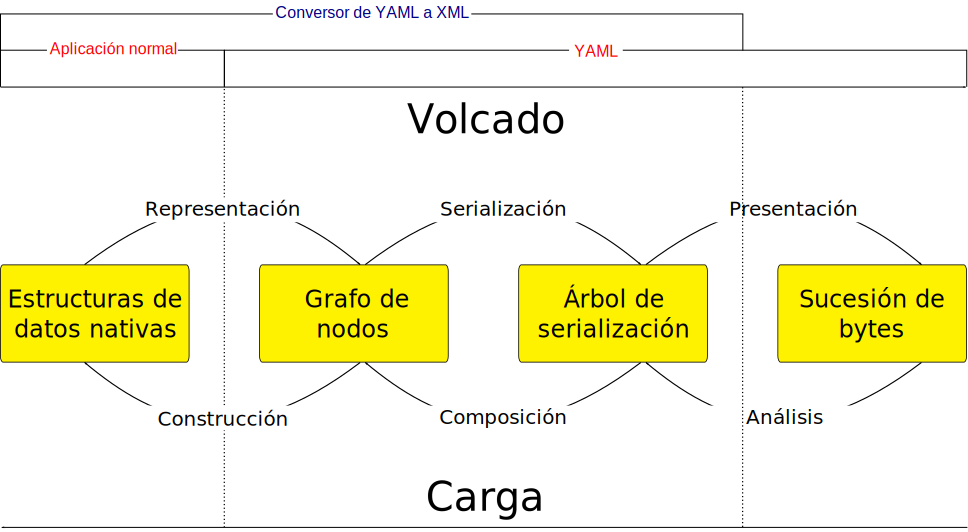
\includegraphics[width=\textwidth]{desarrollo/analisis/procesado_yaml}
  \caption{Secuencia de procesado de \acs{YAML}}
  \label{fig:secuenciaproc_yaml}
\end{figure}

\begin{sidewaysfigure}
  \centering
  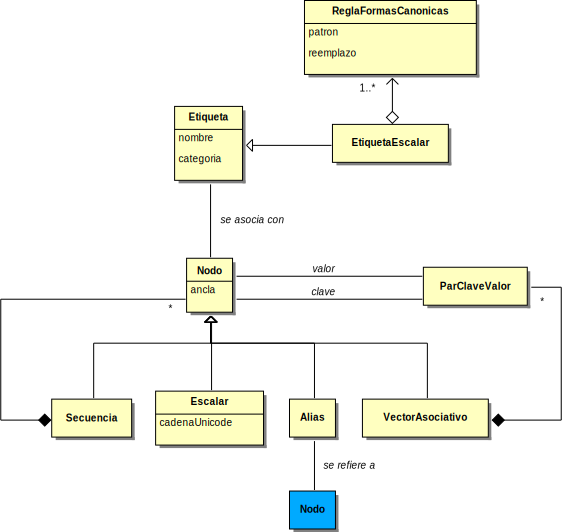
\includegraphics[height=.7\textwidth]{desarrollo/analisis/modyaml}
  \caption{Diagrama de clases conceptuales para \acs{YAML}}
  \label{fig:diaganalisis_yaml}
\end{sidewaysfigure}

\subsubsection{Restricciones textuales}
\label{sec:conceptual_yaml_restricciones}

\begin{itemize}
\item \emph{Clave externa}: ``nombre'' de Etiqueta.
\end{itemize}


%%% Local Variables: 
%%% mode: latex
%%% TeX-master: "../../memoria"
%%% End: 


%%% Local Variables: 
%%% mode: latex
%%% TeX-master: "../../memoria"
%%% End: 


\section{Dise�o del sistema}
\label{sec:diseno}
%%
%% Dise�o
%% Copyright (C) 2008 Antonio Garc�a Dom�nguez
%% $Id: diseno.tex 620 2008-07-01 23:20:02Z antonio $
%% 


\subsection{Arquitectura del sistema}
\label{sec:arquitectura}
%%
%% Arquitectura del sistema
%% Copyright (C) 2008 Antonio Garc�a Dom�nguez
%% $Id: arquitectura.tex 629 2008-07-06 13:47:58Z antonio $
%%

Para poder decidir la arquitectura del sistema, primero habr�a que
definir cu�les son las condiciones que afectar�n a su estructura.

Dichas condiciones se basan tanto en la funcionalidad esperada del
sistema, como en los requisitos no funcionales antes mencionados y
otros factores de calidad del software, como la flexibilidad,
mantenibilidad, reusabilidad o fiabilidad, entre otros.

La mantenibilidad requiere una arquitectura que evite la propagaci�n
de cambios realizados sobre una parte del sistema, definiendo
interfaces estables entre estas partes. Dicha arquitectura debe ser
adem�s lo m�s sencilla posible, para facilitar cambios en su
estructura y elementos.

La divisi�n en partes con l�mites e interfaces bien definidas mejora
tambi�n la reusabilidad y facilita las pruebas, evitando
acoplamientos innecesariamente complejos que dificulten el desarrollo
de una aplicaci�n fiable y con la funcionalidad deseada.

\subsubsection{Separaci�n de responsabilidades: divisi�n en capas}
\label{sec:arquitec_capas}
\index{patr�n arquitect�nico!Capas}
\index{Capas|see{patr�n arquitect�nico!Capas}}

En el caso de este proyecto, se deseaba separar \visor{} de los
detalles de los conversores externos, como \postprocesador{} y
\yaxml{}, y viceversa. En un futuro, se implementar�n nuevas
interfaces de usuario para \visor{}, por lo que tambi�n habr� que
separar la l�gica de aplicaci�n y de presentaci�n de \visor{}.

Bajo este contexto, se puede ver que la aplicaci�n del patr�n
arquitect�nico Capas (descrito con mayor detalle
en~\cite{archpatterns}) es natural. Se ha dividido la aplicaci�n en
cuatro capas:

\begin{description}
\item[Presentaci�n] 
  \index{capa!presentaci�n}

  Se ocupa de la interacci�n persona-m�quina en general y en
  particular de la visualizaci�n de la informaci�n y la navegaci�n a
  trav�s de �sta. Define las transformaciones a realizar sobre las
  representaciones creadas en la capa de filtrado.

\item[Aplicaci�n] 
  \index{capa!aplicaci�n}

  Responde a las peticiones de la capa superior, ejecut�ndolas de
  forma independiente a la interfaz escogida. Implementa la
  infraestructura necesaria para la ejecuci�n de las transformaciones
  de la capa de usuario, posibilitando su selecci�n en tiempo de
  ejecuci�n, enlazado de nodos y localizaci�n de cadenas. Incorpora la
  l�gica necesaria para la integraci�n con los conversores de la capa
  de filtrado.

\item[Filtrado] 
  \index{capa!filtrado}

  A diferencia de la usual capa de dominio en un modelo de tres capas,
  no manipula instancias de los objetos del dominio, sino que los
  transforma a una representaci�n manejable por las capas superiores,
  de ah� su nombre. 

  Se halla constituida por una serie de conversores independientes
  entre s� y de \visor{}, como \postprocesador{} o \yaxml{}. \visor{}
  s�lo ha de conocer la orden a ejecutar, que ha de seguir unas pautas
  muy sencillas:

  \begin{itemize}
  \item El c�digo de retorno de la orden debe indicar el �xito o
    fracaso en la conversi�n.
  \item El resultado \ac{XML} ha de volcarse por la salida est�ndar, y
    el estado de la conversi�n por la salida est�ndar de errores.
  \end{itemize}

\item[Servicios t�cnicos] 
  \index{capa!servicios t�cnicos}

  En esta capa hemos situado todas las bibliotecas, m�dulos externos y
  dem�s que proporcionan parte de la funcionalidad com�n del sistema,
  y son internos a �ste.

\end{description}

Se ha detallado la visi�n en capas (modeladas por paquetes \ac{UML}) a
lo largo del eje vertical y en particiones a lo largo del eje
horizontal en la figura~\ref{fig:arquitec_capas} de la
p�gina~\pageref{fig:arquitec_capas}.

M�s tarde examinaremos cada una de estas capas por separado.

\begin{figure}
  \centering
  \includegraphics[width=.8\textwidth]{desarrollo/diseno/arquitec_capas}
  \caption{Diagrama arquitect�nico del sistema}
  \label{fig:arquitec_capas}
\end{figure}

\subsubsection{Transformaciones configurables: tuber�as y filtros}
\label{sec:tuberias_filtros}
\index{patr�n arquitect�nico!Tuber�as y Filtros}
\index{Tuber�as y Filtros|see{patr�n arquitect�nico!Tuber�as y
    Filtros}}

\paragraph{Descripci�n}

Otro patr�n arquitect�nico usado (con ciertas licencias) en el dise�o
de este proyecto fue Tuber�as y Filtros. Dicho patr�n ser� familiar a
todo usuario de un sistema UNIX, de donde se inspir� precisamente.

Consiste en el encadenamiento de una serie de Filtros, partiendo de
una Fuente de informaci�n, y llegando hasta un Sumidero, destino de la
informaci�n transformada. A cada paso, la informaci�n llega a un
Filtro a trav�s de una Tuber�a, saliendo por otra Tuber�a hacia el
siguiente Filtro o el Sumidero final.

El patr�n original (ver~\cite{archpatterns}) tiene las ventajas de ser
f�cilmente paralelizable en filtros incrementales que no necesiten
leer toda la entrada antes de poder operar, y permitir una gran
flexibilidad cambiando el filtro exacto usado a cada paso, dado que
est�n dise�ados para ser intercambiables entre s�, con ciertas
limitaciones.

Sus desventajas consisten en la dificultad de mantener un estado
compartido y de realizar un control detallado de errores, al ser
usualmente tratada toda la transformaci�n como una unidad.

\paragraph{Uso}

El uso de este patr�n a lo largo de este proyecto se fundament� en la
necesidad de permitir la extensibilidad de la visualizaci�n por parte
del usuario sin necesidad de una recompilaci�n, usando un enfoque
puramente dirigido por datos.

As�, en el caso de una demostraci�n de \ac{ACL2}, si consideramos al
sistema externo \ac{ACL2} como la fuente de la informaci�n y a la
visualizaci�n por parte de la biblioteca Swing como el sumidero,
tendr�amos cuatro filtros intermedios:

\begin{enumerate}
\item \postprocesador{}, con el enunciado Lisp para \ac{ACL2} como
  entrada, genera una representaci�n en \ac{XML} del contenido de la
  demostraci�n realizada. El formato de salida se conoce a trav�s de
  una \ac{DTD}, incrustada en el propio documento de salida.

\item El segundo filtro, definido en la capa de presentaci�n, realiza
  una transformaci�n previa, potencialmente costosa, que afecta a todo
  el documento, y que s�lo se realiza una vez.
  
  Aqu� el usuario puede definir el aspecto que tendr� el �rbol del
  documento, ocultando nodos o cambiando la etiqueta o icono a
  mostrar. La descripci�n de la hoja define las entradas esperadas y
  el formato de la salida.

\item El tercer filtro, tambi�n en la capa de presentaci�n, transforma
  un nodo a su visualizaci�n \ac{XHTML} utilizando una hoja \ac{XSLT}
  para el formato de la salida. La transformaci�n se repite cada vez
  que el usuario cambia de nodo.

  En este caso, se sabe que la salida es \ac{XHTML}, y que sigue por
  lo tanto una \ac{DTD} conocida. Tambi�n podemos deducir a partir del
  nombre de la hoja qu� entrada espera y qu� salida produce.

  As�, sabemos que la hoja \fichero{ppACL2} de visualizaci�n tomar� la
  salida de la hoja de preprocesado \fichero{ppACL2} o una derivada
  suya y mostrar� la informaci�n relevante a demostraciones de
  \ac{ACL2} contenida en dicho documento.

  Una hoja de visualizaci�n es dise�ada suponiendo que la salida del
  preprocesado sigue el formato de salida de ciertas hojas de usuario
  de preprocesado. En el caso contrario, la transformaci�n no fallar�,
  pero no se obtendr�n los resultados esperados.

\item El cuarto filtro, controlado por la capa de aplicaci�n, marca
  las coincidencias de la clave de la b�squeda en curso en el texto,
  si se da el caso. Tambi�n se aplica una hoja de estilos \ac{CSS},
  que no modifica la estructura pero s� el aspecto del resultado
  final.

\end{enumerate}

Como vemos, los dos filtros intermedios se ocupan de la mayor parte de
la visualizaci�n, y seg�n los requisitos funcionales, �stos deber�an
ser modificables por el usuario sin necesidad de recompilaci�n.

\paragraph{Implementaci�n}

\index{XSLT!ventajas}

Se eligi� \ac{XSLT} para implementar estos dos filtros por la
flexibilidad que ofrece al estar basado en ficheros de texto
f�cilmente intercambiables y por su capacidad de describir
declarativamente las transformaciones sobre la fuente \ac{XML} a otros
formatos.

Se opt� por una visualizaci�n basada en \ac{XHTML} para evitar el uso
de numerosos componentes discretos Swing, complicando el dise�o de la
interfaz y las extensiones por parte del usuario. El uso de hipertexto
permite, adem�s de ofrecer mayor informaci�n visual al usuario,
establecer enlaces entre los distintos elementos de la
demostraci�n.

Existen varias diferencias con el patr�n original. Los filtros aqu�
usados no son incrementales (el uso de \ac{XML} no lo permite),
perdi�ndose la capacidad de paralelizaci�n.

Por otro lado, la p�rdida de capacidad de detecci�n detallada de
errores no aparece en nuestro caso, al basarse las tuber�as en l�gica
de la capa de aplicaci�n y no en otros mecanismos de menor nivel de
abstracci�n, como memoria compartida.

No ha sido necesario ning�n estado compartido, por lo que esta otra
desventaja tampoco ha resultado ser ninguna limitaci�n.

\index{translet}

En cuanto a rendimiento, hay que considerar el uso de \emph{translets}
por el procesador \ac{XSLT} Xalan XSLTC. �stos son representaciones
compiladas a bytecode Java de hojas \ac{XSLT} cuya ejecuci�n es
notablemente m�s r�pida que la ejecuci�n interpretada cl�sica, a costa
de cierta funcionalidad innecesaria para este proyecto.

La disposici�n e interconexi�n de los componentes que intervienen en
la transformaci�n se ha recogido en el diagrama \ac{UML} de
componentes de la figura~\ref{fig:componentes_filtros} de la
p�gina~\pageref{fig:componentes_filtros}.

La capa de aplicaci�n no aparece en �l, pero se halla impl�cita, como
capa de control. Tampoco han de confundirse las hojas \ac{XSLT}
usadas, que pertenecen a la capa de presentaci�n, con su l�gica de
control, parte de la capa de aplicaci�n.

\begin{figure}
  \centering
  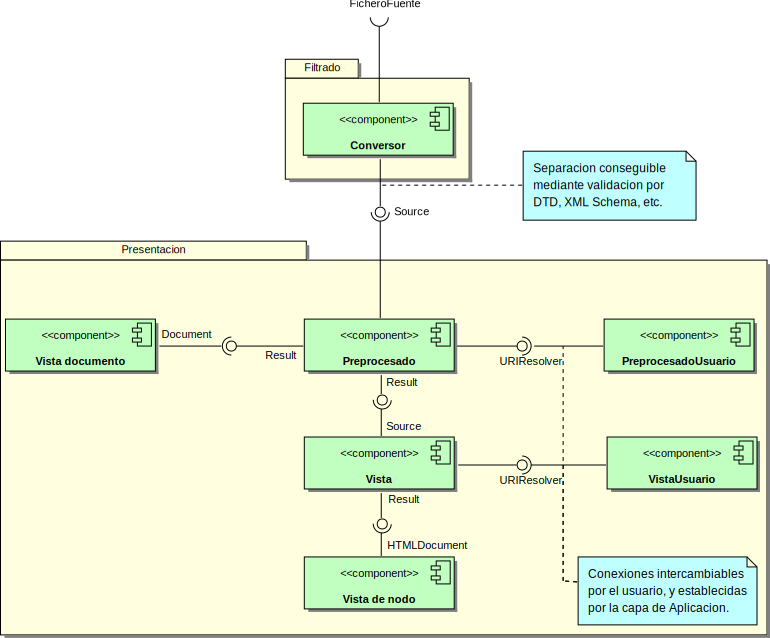
\includegraphics[width=\textwidth]{desarrollo/diseno/componentes}
  \caption{Diagrama de componentes para visualizaci�n}
  \label{fig:componentes_filtros}
\end{figure}

\subsubsection{Integraci�n de las capas de aplicaci�n y presentaci�n: patrones \acs{MVP}}
\label{sec:arquitectura_mvp}

\index{patr�n arquitect�nico!MVC}
\index{patr�n arquitect�nico!MVP}
\index{patr�n arquitect�nico!Controlador Supervisor}
\index{patr�n arquitect�nico!Vista Pasiva}
\index{patr�n arquitect�nico!Modelo de Presentaci�n}
\index{MVC|see{patr�n arquitect�nico!MVC}}
\index{MVP|see{patr�n arquitect�nico!MVP}}
\index{Controlador Supervisor|see{patr�n arquitect�nico!Controlador Supervisor}}
\index{Vista Pasiva|see{patr�n arquitect�nico!Vista Pasiva}}
\index{Modelo de Presentaci�n|see{patr�n arquitect�nico!Modelo de Presentaci�n}}

En el visor del Proyecto que precede a �ste, se hab�a establecido una
comunicaci�n entre las capas de aplicaci�n y de presentaci�n mediante
Fachadas. Estas Fachadas constitu�an el �nico punto de acceso a la
funcionalidad de cada capa, y evitaban que la capa superior tuviera
que conocer los detalles de la capa inferior.

Aunque para sistemas con interfaces m�s sencillos se podr�a haber
continuado su uso, en el caso de \visor{} se vio c�mo las Fachadas
iban tomando demasiadas responsabilidades al mismo tiempo. Tambi�n se
dio el caso de que la capa inferior forzaba a la capa superior a una
serie de restricciones, siendo la m�s grave la de tratar un �nico
documento.

Otro problema que aquejaba al antiguo dise�o es la pr�cticamente nula
capacidad para poder realizar pruebas de unidad de forma c�moda en la
aplicaci�n. Existen herramientas que permiten automatizar pulsaciones
y entrada de teclado, pero las pruebas de este tipo son extremadamente
fr�giles: cualquier cambio en la disposici�n de los controles de la
interfaz las invalidar�a.

Para resolver ambos problemas, se estudiaron las diversas alternativas
ofrecidas en~\cite{Fowler:GUIArch}, y en particular las derivaciones
del patr�n \ac{MVP}. Este patr�n es una derivaci�n del
\ac{MVC}~\cite{gof} original en el que en vez de tener un tr�o
modelo-vista-controlador para cada control de la interfaz (como un
campo de texto, por ejemplo), tenemos un tr�o para el formulario
completo. Ahora el modelo del formulario es el conjunto de clases del
dominio usadas, la vista es la estructura formada por todos los
controles gr�ficos del formulario, y el presentador es el componente
al que se notifican todas las acciones de inter�s realizadas por el
usuario.

El presentador es el ocupado de modificar el modelo, y posteriormente
la vista se actualizar� con los cambios hechos por el presentador al
modelo. Hay diversos mecanismos para garantizar esta sincronizaci�n,
constituyendo variantes distintas del patr�n \ac{MVP} b�sico:

\begin{description}
\item[Controlador Supervisor] Para los casos simples, la
  sincronizaci�n modelo-vista se establece a partir del patr�n
  Observador o alg�n otro enfoque declarativo. En casos m�s complejos,
  el presentador interviene directamente sobre los controles de la
  interfaz.

\item[Vista Pasiva] La vista en este caso carece de cualquier l�gica
  de sincronizaci�n, y es el presentador el que rellena todos los
  campos. Una posibilidad para evitar acoplar demasiado el presentador
  a los controles usados es definir una interfaz en el formulario para
  su relleno: de esta forma, durante las pruebas de unidad podemos
  sustituir la vista por un Doble para Pruebas~\cite{Meszaros:XUnit} y
  depurar pr�cticamente toda la funcionalidad.

\item[Modelo de Presentaci�n] El presentador contiene el estado
  abstracto que deber�a presentar el formulario. Puede que sea el
  modelo de presentaci�n el que manipule la vista, o que sea la vista
  la que se actualice a partir del modelo de presentaci�n. En el
  primer caso, ambos elementos est�n m�s acoplados pero podemos probar
  la sincronizaci�n. En el segundo caso, la sincronizaci�n no se puede
  depurar tan f�cilmente, pero el modelo de presentaci�n es
  completamente independiente de la interfaz usada.

\end{description}

De entre estos enfoques, se escogi� el Modelo de Presentaci�n, ya que
en un futuro se desean crear nuevas interfaces para \visor{}: el
presentador no deber�a de saber nada acerca de la vista. Por la misma
raz�n, es la vista la que se actualiza al estado encapsulado por el
modelo de presentaci�n.

El uso de un modelo de presentaci�n tambi�n facilita la implementaci�n
de una interfaz multidocumento: cada documento puede imponer su propio
estado de presentaci�n sin afectar a los dem�s.

En cuanto a la divisi�n en modelo-vista-presentador, tendr�amos a los
modelos y otros servicios de alto nivel en la capa de aplicaci�n, y a
las vistas y presentadores en la capa de presentaci�n.

%%% Local Variables: 
%%% mode: latex
%%% TeX-master: "../../memoria"
%%% End: 


\subsection{Capa de filtrado: \nombrepostprocesador{}}
\label{sec:capa_filtrado_acl2}
%%
%% Capa de filtrado: ACL2
%% Copyright (C) 2008 Antonio Garc�a Dom�nguez
%% $Id: capa_filtrado_acl2.tex 629 2008-07-06 13:47:58Z antonio $
%%

Volviendo al diagrama de capas de la figura~\ref{fig:arquitec_capas}
de la p�gina~\pageref{fig:arquitec_capas}, vemos que este conversor ha
de:
\begin{itemize}
\item Convertir la salida de \ac{ACL2} a \ac{XML} sin p�rdidas.
\item Definir claramente el formato de dicha salida.
\end{itemize}

Por la necesidad de manipular el texto de la forma m�s sencilla y
potente posible, se escogi� usar un gui�n escrito en Perl, un lenguaje
dise�ado a este efecto.

A ra�z de la complejidad inherente en el manejo de la salida en
lenguaje humano de un programa como \ac{ACL2}, se ha seguido el
paradigma orientado a objetos a la hora de desarrollar
\postprocesador{}.

\subsubsection{Procesado general de proyectos de \acs{ACL2}}
\label{sec:postproc_estruc_general}

El dise�o b�sico se fundamenta en el modelo conceptual de datos, con
ciertas modificaciones. El gui�n lanzado por la capa de aplicaci�n
emplea la funci�n \funcion{convertir\_a\_xml} del m�dulo
\clase{Procesador}, pas�ndole la ruta al \clase{Enunciado} ra�z del
proyecto completo, y vuelca sus resultados por la salida est�ndar.

Este m�todo es realmente un envoltorio que crea un \clase{Proyecto}
con ra�z en el \clase{Enunciado} indicado, actualiza por completo de
forma recursiva todas las salidas de \ac{ACL2} y sus versiones en
\ac{XML} y devuelve la versi�n \ac{XML} de la salida de la ra�z del
proyecto.

Las \clase{Dependencias} del \clase{Proyecto} son obtenidas a partir
de un an�lisis est�tico del c�digo Lisp, empezando por el
\clase{Enunciado} Lisp ra�z y continuando de forma recursiva. Esto
genera un �rbol anidado de \clase{Proyecto}s que dependen unos de
otros. Decimos �rbol y no grafo pues un subproyecto puede aparecer
varias veces en el mismo �rbol. Esto supone un coste mayor en espacio,
pero no en tiempo: si tuviera que ser actualizado, s�lo ser�a
procesado una vez. Se est�n considerando representaciones m�s
eficientes en espacio para versiones posteriores.

El proceso de actualizaci�n consiste en recorrer el �rbol e ir
actualizando de forma recursiva:

\begin{enumerate}
\item Se solicita la actualizaci�n de las \clase{Dependencias} del
  proyecto actual, que forman \clase{Proyecto}s a su vez.

\item Si alg�n subproyecto fue actualizado o el fichero temporal con
  la salida de \ac{ACL2} no existe o tiene una fecha de modificaci�n
  m�s antigua que la del \clase{Enunciado}, se invocar� a \ac{ACL2}
  para crear o actualizar dicho fichero temporal.

\item Si el fichero temporal con la salida fue actualizado o el
  fichero temporal con el documento \ac{XML} resultante no existe o
  tiene una fecha de modificaci�n m�s antigua que la de la salida, se
  actualizar� empleando una instancia de la clase
  \clase{Demostraci�n}, que encapsula el proceso de an�lisis de una
  demostraci�n de \ac{ACL2}.
\end{enumerate}

El diagrama de secuencia correspondiente a esta l�gica se halla en el
cuadro~\ref{fig:ds_filtrado_general} de la
p�gina~\pageref{fig:ds_filtrado_general}. El diagrama con las clases
participantes, integradas con las ocupadas de procesar las
\clase{Demostracion}es en s�, forma el
cuadro~\ref{fig:diag_clases_diseno_pproc} de la
p�gina~\pageref{fig:diag_clases_diseno_pproc}.

\begin{sidewaysfigure}
  \centering
  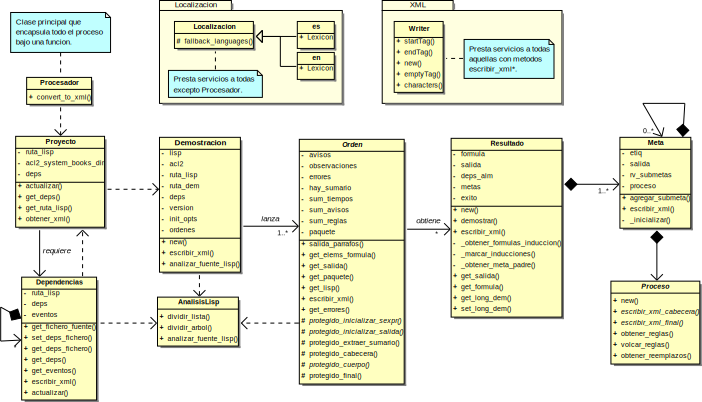
\includegraphics[width=\textwidth]{desarrollo/diseno/clases_acl2proc_general}
  \caption{Diagrama de clases de \postprocesador{} (general)}
  \label{fig:diag_clases_diseno_pproc}
\end{sidewaysfigure}

\begin{sidewaysfigure}
  \centering
  \includegraphics[width=\textwidth]{desarrollo/diseno/diag_sec_acl2proc_general}
  \caption{Diagrama de secuencia general de filtrado}
  \label{fig:ds_filtrado_general}
\end{sidewaysfigure}

\subsubsection{Generaci�n de modelos en memoria}

Un concepto importante para comprender el dise�o de \postprocesador{}
en esta versi�n es la necesidad cada vez mayor de atrasar el momento
de la generaci�n de la salida \ac{XML}. Originalmente, ambos estaban
intercalados. Sin embargo, en muchos casos el orden en que se procesa
la informaci�n no coincide con el orden en que se debe producir la
salida, y esto supon�a un impedimento para el procesamiento de
demostraciones cada vez m�s complejas.

A lo largo de las iteraciones, se ha hecho una divisi�n mayor y mayor,
hasta finalmente separar el procesado y la salida a nivel de una
\clase{Demostraci�n} completa, en vez de \clase{Resultado}s
individuales.  Esto permite dar nuevos usos al an�lisis ya
implementado. Puede verse esta separaci�n en el diagrama de secuencia
de la figura~\ref{fig:ds_filtrado_demo} de la
p�gina~\pageref{fig:ds_filtrado_demo}: la inicializaci�n se hace s�lo
durante la ejecuci�n del constructor \metodo{new}, y la salida se
produce exclusivamente dentro del m�todo \metodo{escribir\_xml}.

Por ejemplo, se puede analizar una \clase{Demostraci�n} sin contar con
su salida, realizando un an�lisis est�tico sobre el c�digo Lisp: toda
\clase{Orden} dispone de m�todos separados para recuperar informaci�n
de la S-expresi�n y de la salida de \ac{ACL2}, y el �ltimo s�lo es
usado cuando se proporciona dicha salida en el constructor. Este
an�lisis est�tico proporciona informaci�n de todas las dependencias de
un proyecto.

\begin{sidewaysfigure}
  \centering
  \includegraphics[width=.8\textwidth]{desarrollo/diseno/diag_sec_acl2proc_demostracion}
  \caption{Diagrama de secuencia de filtrado de una \clase{Demostraci�n}}
  \label{fig:ds_filtrado_demo}
\end{sidewaysfigure}

\subsubsection{Relaci�n con capa de servicios t�cnicos}
\label{sec:postproc_servtecnicos}
\index{�rbol Perl}

Viendo el diagrama general de clases de dise�o para la capa de
filtrado, se puede observar que la mayor�a de las clases tienen
dependencias con \clase{XML::Writer} y \clase{Localizaci�n}.

Esto es lo usual con los elementos de la capa de servicios t�cnicos:
\clase{XML::Writer} es un m�dulo usado para la salida \ac{XML}, que
incorpora ciertas comprobaciones autom�ticas para garantizar la
ejecuci�n de generaci�n de documentos bien formados, y
\clase{Localizaci�n} es el m�dulo usado para localizaci�n de mensajes
de error o avisos.

No hay que confundir dichos servicios t�cnicos con clases de utilidad
como \clase{An�lisisLisp}, que a�sla la l�gica necesaria para
convertir listas y �rboles Lisp a estructuras de datos equivalentes de
Perl.

\subsubsection{Reflexi�n y tipos basados en comportamiento:
  simplificaci�n del an�lisis est�tico}
\label{sec:acl2proc_reflexion}

Al implementar el an�lisis est�tico necesario para conseguir el grafo
de dependencias de un proyecto, surge la necesidad de conocer cu�l
ser�a el identificador final y paquete de cada evento, y de las rutas
de todos los libros. Evidentemente, hay que distinguir entre los
\clase{Evento}s con nombre, los \clase{Evento}s sin nombre y los
\clase{NoEvento}s, que no producen cambios en el mundo l�gico de
\ac{ACL2}.

Sin embargo, se desea conservar toda la l�gica propia a cada orden en
su propia subclase de \clase{Orden}. La forma m�s l�gica ser�a a�adir
niveles a la estructura de herencia, distinguiendo as� entre los
\clase{Evento}s con nombre, los \clase{Evento}s sin nombre y los
\clase{NoEvento}s, pero esto s�lo resolver�a parte del problema:
seguir�amos teniendo que preguntar si la \clase{Orden} usada pertenece
a la lista de aquellas que afectan al paquete actual, o de la lista de
\clase{Orden}es ocupadas del manejo de libros. Tendr�amos entonces que
utilizar herencia m�ltiple. Como vemos, preguntar por la subclase
exacta de la \clase{Orden} seg�n el criterio que necesitemos en un
momento determinado a�ade una complejidad al c�digo y crea un
acoplamiento mucho mayor de lo esperado.

\index{duck typing}

La alternativa se halla en el concepto conocido como ``duck
typing''~\cite{Martelli2000}, muy popular en lenguajes con sistemas de
tipos din�micos como Python, y defendido (aunque no bajo ese mismo
nombre) por autores como Bruce Eckel~\cite{EckelDuckTyping}. La
definici�n del glosario de Python~\cite{DuckTyping} es la siguiente:

\begin{quotation}
  Pythonic programming style that determines an object's type by
  inspection of its method or attribute signature rather than by
  explicit relationship to some type object ("If it looks like a duck
  and quacks like a duck, it must be a duck.") By emphasizing
  interfaces rather than specific types, well-designed code improves
  its flexibility by allowing polymorphic substitution. Duck-typing
  avoids tests using type() or isinstance(). Instead, it typically
  employs hasattr() tests or EAFP programming.
\end{quotation}

Es decir, no distinguimos a los tipos por ``qui�nes'' son, con
\verb#instanceof# en Java o \verb#typeid# en \CPP, por ejemplo, y
luego hacemos \emph{upcasting} a una clase o interfaz com�n. En su
lugar, los distinguimos por c�mo se comportan: si \verb#anda()# como
un \clase{Pato} y \verb#hace_cuac()# como un \clase{Pato}, entonces es
un \clase{Pato} para nuestro c�digo.

Se podr�a ver el ``duck typing'' como una versi�n de la programaci�n
gen�rica de \CPP en que la comprobaci�n de tipos se hace en tiempo de
ejecuci�n y s�lo se requieren aquellos m�todos que son realmente
usados, en vez de todos las que aparecen en el c�digo.

\index{EAFP}

Existen dos estilos para su implementaci�n, como sugiere la definici�n
anterior. El segundo estilo hace referencia al acr�nimo \ac{EAFP}:
asumimos que los m�todos necesarios se implementan y capturamos los
errores si nos equivocamos. Dado que en el an�lisis est�tico se
mezclan las \clase{Orden}es que cumplen o no cada uno de los criterios
libremente, este m�todo no nos sirve: el manejo de excepciones no es
un mecanismo de control de flujo, al fin y al cabo.

\index{reflexi�n}

El primer m�todo s� es �til, pero notemos que hace uso de algo que no
todo lenguaje tiene: la capacidad de consultar y operar sobre la
propia estructura del programa, en tiempo de ejecuci�n. Dicho proceso
es conocido como \emph{reflexi�n}, y se halla integrado dentro de
muchos lenguajes, como Java, C\#, Perl o Python.

As�, el an�lisis est�tico asume que si una clase implementa el m�todo
\metodo{get\_nombre\_paquete} cambia el paquete actual, si implementa
\metodo{get\_identificador\_evento} representa a un \clase{Evento} con
un nombre referenciable posteriormente, y si implementa el m�todo
\metodo{get\_ruta\_libro}, que de alguna forma ha incluido los
contenidos del libro bajo la ruta especificada bajo el mundo l�gico de
\ac{ACL2}.

\subsubsection{Patr�n M�todo F�brica: creaci�n de �rdenes y Procesos}
\label{sec:postproc_patron_fabrica}
\index{patr�n de dise�o!M�todo F�brica}
\index{M�todo F�brica|see{patr�n de dise�o!M�todo F�brica}}

Se us� el patr�n \patron{M�todo F�brica} de~\cite{gof} para aislar
al resto del post-procesador de la l�gica necesaria para identificar
qu� tipo de \clase{Orden} o \clase{Proceso} hay que crear exactamente.

Podemos ver en el diagrama de clases de dise�o general de la
figura~\ref{fig:diag_clases_diseno_pproc} en la
p�gina~\pageref{fig:diag_clases_diseno_pproc} dos clases abstractas,
\clase{Orden} y \clase{Proceso}. Las instancias de sus subclases se
crean mediante los m�todos \metodo{crear} de
\clase{ACL2::Orden::Fabrica} y \clase{ACL2::Proceso::Fabrica}.

\index{paquete Lisp}

En ambos casos, son los valores de los argumentos proporcionados los
que determinan qu� subclase concreta de la clase abstracta base se va
a crear. En el caso de \clase{Orden}, se env�a la S-expresi�n, el
paquete Lisp actual y la salida. En el caso de \clase{Proceso}, se
env�a la salida.

\clase{ACL2::Proceso::Fabrica} requiere algo m�s de participaci�n por
parte de las subclases de Proceso. Todas deben registrar una subrutina
an�nima que determine si la salida enviada por \clase{Meta} se
corresponde con ella, y que devuelva los par�metros requeridos al
constructor en dicho caso. Esto podr�a considerarse como un uso del
patr�n \patron{Orden}, descrito en m�s detalle en la capa de
presentaci�n.

Dicha f�brica queda as� como un punto central f�cilmente accesible por
\clase{Meta} de creaci�n de \clase{Proceso}s, y la l�gica espec�fica a
cada proceso se halla concentrada y separada del resto en un �nico
fichero.


\subsubsection{Patr�n M�todo Plantilla}
\label{sec:postproc_patron_metplantilla}
\index{patr�n de dise�o!M�todo Plantilla}
\index{M�todo Plantilla|see{patr�n de dise�o!M�todo Plantilla}}
\index{operaciones de enganche}

Este patr�n, tambi�n proveniente de~\cite{gof}, se usa en la jerarqu�a
de \clase{Orden} para reunir todo el comportamiento com�n en el
filtrado de las �rdenes.

Toda orden en \ac{ACL2} produce una serie de mensajes de error, aviso
u observaci�n. Tambi�n se a�ade usualmente (pero no siempre) un
sumario, cuyo formato es fijo en toda orden. Se da adem�s que la
l�gica de manejo de errores de \ac{ACL2} es siempre la misma.

Toda esta l�gica com�n es reunida en un m�todo de una clase base, que
emplea una serie de ``operaciones de enganche'' protegidas, que
permiten especializar mediante herencia partes de ese m�todo con la
l�gica espec�fica para cada orden, facilitando a�adir nuevas �rdenes o
modificar las existentes. El nombre de ``m�todo plantilla'' viene de
esa capacidad de rellenar los ``huecos'' de su l�gica.

\clase{Orden} dispone de dos m�todos plantilla:

\begin{enumerate}
\item \metodo{inicializar} dispone de los enganches:
  \begin{itemize}
  \item \metodo{protegido\_inicializar\_sexpr}: operaci�n abstracta.
  \item \metodo{protegido\_inicializar\_salida}: operaci�n abstracta.
  \item \metodo{protegido\_extraer\_sumario}: tiene una implementaci�n
    por defecto.
  \end{itemize}

\item \metodo{escribir\_xml} se puede especializar a partir de:

  \begin{itemize}
  \item \metodo{protegido\_cabecera}: tiene una implementaci�n por
    defecto.
  \item \metodo{protegido\_cuerpo}: operaci�n abstracta.
  \item \metodo{protegido\_final}: tiene una implementaci�n por
    defecto.
  \end{itemize}
\end{enumerate}

El uso del prefijo ``\metodo{protegido\_}'' en los nombres se trata de
un esquema de nombrado, siguiendo la pr�ctica com�n en muchos m�dulos
del \ac{CPAN}, y no implica la existencia de un mecanismo de control
de acceso real, por sencillez.

\subsubsection{Jerarqu�a de �rdenes}
\label{sec:postproc_jerarq_ordenes}

El diagrama de clases de dise�o \ac{UML} puede verse en la
figura~\ref{fig:postproc_jerarq_ordenes} de la
p�gina~\pageref{fig:postproc_jerarq_ordenes}.

Puede verse como cada clase redefine los m�todos de enganche
necesarios, a�adiendo algunas operaciones privadas para su propia
funcionalidad.

\begin{figure}
  \centering
  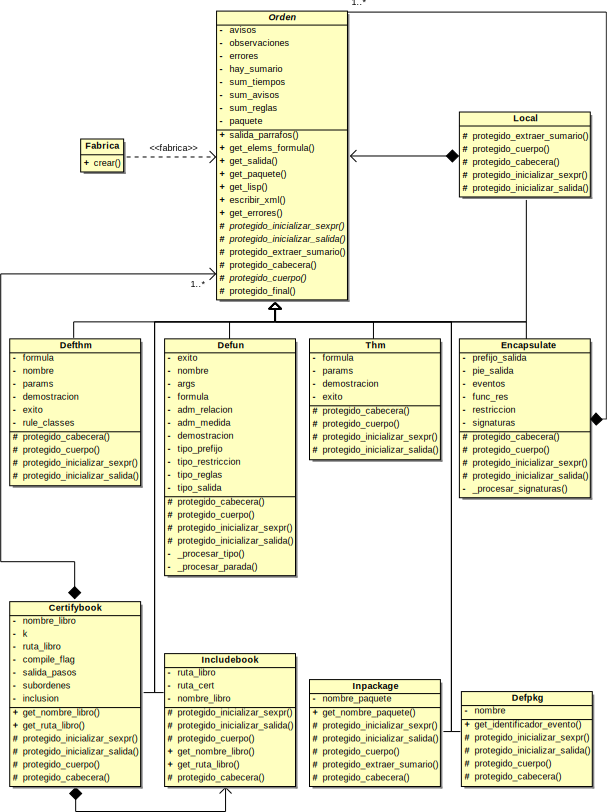
\includegraphics[width=\textwidth]{desarrollo/diseno/clases_acl2proc_ordenes}
  \caption{Diagrama de clases de �rdenes de \postprocesador{}}
  \label{fig:postproc_jerarq_ordenes}
\end{figure}

\subsubsection{Jerarqu�a de Procesos}
\label{sec:postproc_jerarq_procesos}

El diagrama de esta jerarqu�a se halla en la
figura~\ref{fig:postproc_jerarq_procesos} de la
p�gina~\pageref{fig:postproc_jerarq_procesos}.

Los m�todos privados est�ticos \metodo{\_identificar} contienen el
c�digo que se registra en la \clase{F�brica}, utilizando una subrutina
an�nima (parecida a una clausura lambda). Para ocultar los detalles,
\clase{F�brica} emula en su m�todo \metodo{registrar} control de
acceso por paquete.

\begin{figure}
  \centering
  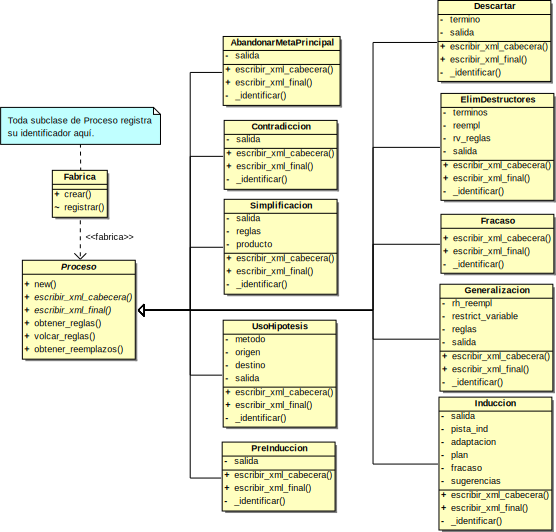
\includegraphics[width=\textwidth]{desarrollo/diseno/clases_acl2proc_procesos}
  \caption{Diagrama de clases de Procesos de \postprocesador{}}
  \label{fig:postproc_jerarq_procesos}
\end{figure}

\subsubsection{Un ejemplo: definici�n de teorema}
\label{sec:postproc_ejemplo_defthm}

Para explicar en m�s detalle qu� es lo que se requiere para el
filtrado de una orden de \ac{ACL2}, usaremos como ejemplo el procesado
de un supuesto evento de definici�n de un teorema, \texttt{defthm}.

\index{patr�n de dise�o!F�brica Abstracta}

Tras crearse la \clase{Orden} a trav�s de la \patron{F�brica
  Abstracta} \clase{Orden::Fabrica}, se generar� la versi�n \ac{XML}
de la salida de \ac{ACL2} en dos pasos. Cada paso se corresponde con
uno de los m�todos plantilla antes mencionados.

En primer lugar, se captura toda la informaci�n disponible en la
salida de \ac{ACL2} (si se proporciona) y la S-expresi�n original
mediante \metodo{inicializar}:

\begin{enumerate}
\item \metodo{\_init\_desde\_salida} definido por \clase{Orden} retira
  toda la informaci�n de la salida no espec�fica a la \clase{Orden}
  \clase{Defthm}, simplificando as� su inicializaci�n.

  Ello incluye retirar los mensajes de \ac{ACL2}, los mensajes del
  colector de basura del int�rprete Lisp y el sumario de la ejecuci�n
  de la orden.

\item \metodo{protegido\_inicializar\_sexpr}, propio de
  \clase{Defthm}, obtiene informaci�n espec�fica a \clase{Defthm} a
  partir de su S-expresi�n:

  \begin{itemize}
  \item F�rmula a demostrar.

  \item Nombre del teorema.

  \item Clases de regla a generar, con el valor por defecto
    ``:REWRITE'', indicando que se usar� una regla de reescritura de
    miembros.

  \item Activaci�n o desactivaci�n de la bandera OTF (``on through the
    fog''), obligando a \ac{ACL2} a que, si con s�lo simplificar no
    basta, no intente inducir sobre la f�rmula original, sino sobre
    las m�ltiples f�rmulas resultantes de las simplificaciones.

  \item Captura de otros argumentos de inter�s.
  \end{itemize}

\item \metodo{protegido\_inicializar\_salida}, definido por
  \clase{Defthm}, se ocupa de recabar toda la informaci�n de inter�s
  del texto de la salida de \ac{ACL2}. Nos interesan las dependencias
  de almacenamiento de las reglas generadas, y los pasos de la
  demostraci�n realizada.

  En primer lugar, recuperaremos la informaci�n mediante el m�todo
  plantilla \metodo{inicializar}:

  \begin{enumerate}
  \item Obtener cada una de las metas e inicializarlas. Tras dividir
    la salida completa en la salida de cada meta, se emplear� el
    \patron{M�todo F�brica} \metodo{crear} de
    \clase{Proceso::Fabrica}, que invocar� a las subrutinas an�nimas
    registradas para reconocer e instanciar el \clase{Proceso} exacto
    seguido.

    Cada meta introducida se guardar� en un vector asociativo para el
    siguiente paso, utilizando su etiqueta, como ``Subgoal *1''.

  \item Organizar jer�rquicamente las metas. 

    Esto se puede hacer f�cilmente a partir de las etiquetas: una meta
    con la etiqueta ``Subgoal *1.1'' tiene como padre la meta con la
    etiqueta ``Subgoal *1'', por ejemplo.

    Gracias al vector asociativo anterior, s�lo hay que calcular la
    etiqueta del padre, recuperarlo y a�adirle la submeta.
  \end{enumerate}
\end{enumerate}

A continuaci�n, invocaremos al otro m�todo plantilla,
\metodo{escribir\_xml}, para obtener el documento \ac{XML} que lista
toda la informaci�n antes recogida:
  
\begin{enumerate}
\item \metodo{protegido\_cabecera}: escritura de la cabecera de la
  salida \ac{XML} correspondiente al \texttt{defthm}. Se abre un nuevo
  elemento \texttt{defthm} mediante \metodo{startTag} de
  \clase{XML::Writer}.

\item \metodo{\_escribir\_mensajes}: este m�todo es parte de la
  funcionalidad implementada por \clase{Orden}, y vuelca los mensajes
  de \ac{ACL2}: avisos, observaciones y errores.

\item \metodo{protegido\_cuerpo}: escritura del cuerpo de la salida
  \ac{XML} del \texttt{defthm}. Se vuelca la informaci�n conseguida
  antes en \metodo{protegido\_inicializar}, incluyendo la
  demostraci�n, delegando en el m�todo \metodo{escribir\_xml} de
  \clase{Resultado}.

\item \metodo{\_escribir\_sumario}: tambi�n parte de la funcionalidad
  predefinida por \clase{Orden}, vuelca el sumario de la ejecuci�n del
  evento, incluyendo tiempos, reglas usadas y avisos dados.

\item \metodo{protegido\_final}: en este caso, \texttt{defthm} no
  redefine la funcionalidad predefinida por \clase{Orden}, cerr�ndose
  el elemento inicial escrito en \metodo{protegido\_cabecera} con un
  elemento del mismo nombre que la orden.
\end{enumerate}

Se ha descrito tambi�n de manera gr�fica este proceso utilizando
diagramas de secuencia \ac{UML} 1.4. Se necesit� dividir el diagrama
en dos: el primero, dedicado al an�lisis, es la
figura~\ref{fig:ds_filtrado_defthm} de la
p�gina~\pageref{fig:ds_filtrado_defthm}, y el segundo, dedicado a la
salida, es la figura~\ref{fig:ds_filtrado_defthm_2} de la
p�gina~\pageref{fig:ds_filtrado_defthm_2}.

Por razones de espacio, algunas de las l�neas de vida no se extienden
hasta el final de la hoja, sin que esto implique su destrucci�n. El
nivel de detalle escogido no describe las operaciones internas de
\clase{Orden} o \clase{Defthm} que no requieran interacci�n por parte
de otras clases, o los mensajes de poco inter�s enviados a
\clase{XML::Writer}.

Los vectores asociativos de Perl han sido modelados como objetos de la
clase \clase{Hash}, por uniformidad.

\begin{sidewaysfigure}
  \centering
  \includegraphics[width=\textwidth]{desarrollo/diseno/diag_sec_acl2proc_defthm_analisis}
  \caption{Diagrama de secuencia de filtrado de \texttt{defthm} (an�lisis)}
  \label{fig:ds_filtrado_defthm}
\end{sidewaysfigure}

\begin{sidewaysfigure}
  \centering
  \includegraphics[width=\textwidth]{desarrollo/diseno/diag_sec_acl2proc_defthm_salida}
  \caption{Diagrama de secuencia de filtrado de \texttt{defthm} (generaci�n de salida)}
  \label{fig:ds_filtrado_defthm_2}
\end{sidewaysfigure}

%%% Local Variables: 
%%% mode: latex
%%% TeX-master: "../../memoria"
%%% End: 


\subsection{Capa de filtrado: \nombreyaxml{}}
\label{sec:capa_filtrado_yaxml}
%
% Capa de filtrado: YAXML::Reverse
% Copyright (C) 2008 Antonio Garc�a Dom�nguez
% $Id$

\subsubsection{Descripci�n general}
\label{sec:descripcion_general}

Este conversor implementa la correspondencia \ac{XML} $\rightarrow$
\ac{YAML} conocida como \ac{YAXML}~\cite{YAXML} en sentido inverso,
con dos objetivos en general:

\begin{itemize}
\item En primer lugar, para permitir a \visor{} abrir cualquier
  documento basado en el metalenguaje \ac{YAML}, o su subconjunto
  (desde \ac{YAML} 1.1) \ac{JSON}. Ello permitir� tratar una familia
  completa nueva de formatos.

\item En segundo lugar, para todos aquellos que necesiten aplicar
  alguna herramienta a sus documentos que no est� disponible para
  \ac{YAML}, como transformaciones definidas de forma funcional
  mediante \ac{XSLT}.
\end{itemize}

El proceso es relativamente sencillo:

\begin{enumerate}
\item Se analiza el documento origen \ac{YAML}, deserializ�ndose a una
  estructura de datos Perl. Este primer paso se consigue mediante el
  m�dulo Perl \modulo{YAML::XS}, un \emph{binding} que permite
  aprovechar la funcionalidad de la biblioteca \verb#libyaml#
  (disponible en \url{http://pyyaml.org/wiki/LibYAML}), y analizar
  documentos \ac{YAML} 1.1 y \ac{JSON}. Existen una serie de
  restricciones, que veremos posteriormente en el
  apartado~\ref{sec:limitaciones} de la
  p�gina~\pageref{sec:limitaciones}.

\item Se representa dicha estructura como un �rbol \ac{XML}, con una
  versi�n mejorada del formato sugerido por \ac{YAXML} para tratar
  ciertos casos especiales.
\end{enumerate}

Sin embargo, hay una serie de detalles de inter�s en la inversi�n de
\ac{YAXML} que consideramos merece la pena mencionar. Tambi�n se han
encontrado algunas limitaciones debidas en primer lugar al m�dulo
\modulo{YAML::XS}, y en �ltima instancia al propio lenguaje Perl, pero
se estima que tendr�n realmente poco impacto en su uso.

\subsubsection{Regeneraci�n de anclas y alias en el fichero \acs{XML}}
\label{sec:anclas_alias_xml}

Hay una diferencia muy importante en los modelos de informaci�n
com�nmente usados en \ac{YAML} y \ac{XML}: el modelo de informaci�n de
presentaci�n de \ac{YAML}, tal y como se coment�
en~\S\ref{sec:modinf_yaml} (p�gina~\pageref{sec:modinf_yaml}), utiliza
grafos dirigidos con ra�z, y el modelo \ac{DOM} com�nmente usado en \ac{XML}
emplea �rboles. Esto implica dos problemas, fundamentalmente:

\begin{itemize}
\item Un primer problema, de menor importancia, es el hecho de que si
  un nodo del grafo tiene varios arcos entrantes, tendr� que ser
  repetido varias veces en el �rbol final. Este problema se agrava
  cuando el nodo a repetir no es un nodo hoja, sino un nodo ra�z de un
  subgrafo: tendremos que repetir el subgrafo completo. De todas
  formas, este problema es m�s una cuesti�n de eficiencia, y en
  ciertos casos se podr�a incluso aceptar el coste adicional.

\item El problema mayor es que en los grafos de \ac{YAML}, se admiten
  ciclos: no existe forma de representar directamente estas
  estructuras c�clicas en un �rbol \ac{XML}.
\end{itemize}

\index{YAML!ancla}
\index{YAML!alias}

La forma en que \ac{YAXML} resuelve estos problemas es utilizando no
el modelo de informaci�n de representaci�n, sino el modelo de
informaci�n de serializaci�n, que s� est� basado en �rboles. En dicho
modelo, se definen los conceptos de \emph{ancla} y de \emph{alias},
pudiendo as� establecer enlaces entre los nodos del �rbol, y resolver
los dos problemas anteriores. En \ac{YAXML}, se representan como
atributos de un elemento sin contenido (como \verb#<a/>#). Pueden
compararse los resultados para un caso sencillo en la
figura~\ref{fig:grafos_mediante_arboles} de la
p�gina~\pageref{fig:grafos_mediante_arboles}.

Existe un problema, sin embargo: utilizando \modulo{YAML::XS}, lo que
obtenemos es el grafo final. Para reconstruir el �rbol con anclas y
alias a partir del grafo, hemos de distinguir qu� elementos del grafo
constituyen anclas y qu� elementos constituyen alias a esas
anclas. Podemos aprovechar el hecho de que la estructura creada por
\modulo{YAML::XS} se basa en referencias a direcciones de memoria con
vectores asociativos, listas y objetos: si en dos o m�s puntos del
�rbol aparecen referencias a la misma direcci�n de memoria, sabremos
que la primera aparici�n ser� el ancla, y todas las dem�s ser�n sus
alias.

El mayor problema es que no sabremos si un nodo constituye un ancla
hasta que sea usado como tal por primera vez en cualquier otro punto
del documento. Por ello, tendremos entonces que dividir la generaci�n
de la salida en dos pasos:

\begin{enumerate}
\item En una primera pasada, se recopila en un vector asociativo qu�
  referencias constituyen anclas, junto con su posici�n en orden de
  uso, a partir de la cual se generar� el identificador final.

\item En la segunda pasada, se genera el c�digo \ac{XML}, cuidando de
  generar los atributos \verb#anchor# y \verb#alias# en los nodos
  apropiados.
\end{enumerate}

\begin{figure}
  \centering
  \mbox{\subfigure[Grafo original]{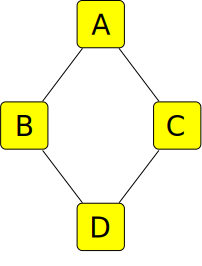
\includegraphics[width=.3\textwidth]{desarrollo/diseno/grafos_yaml_original}}\quad
    \subfigure[�rbol sin enlaces]{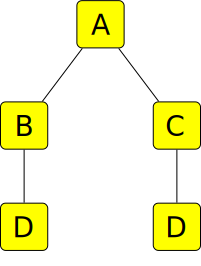
\includegraphics[width=.3\textwidth]{desarrollo/diseno/grafos_yaml_arbolsinenlaces}}\quad
    \subfigure[�rbol con enlaces]{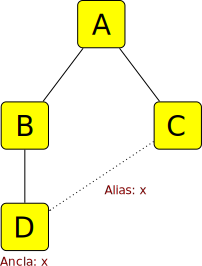
\includegraphics[width=.3\textwidth]{desarrollo/diseno/grafos_yaml_arbolconenlaces}}\quad
  }
  \caption{Representaci�n de grafos mediante �rboles XML}
  \label{fig:grafos_mediante_arboles}
\end{figure}

\subsubsection{Pruebas de unidad autom�ticas basadas en equivalencia}
\label{sec:yaxml_equivalencia}

\index{or�culo}

Un problema fundamental en la realizaci�n de pruebas de software es la
elaboraci�n de los \emph{or�culos}~\cite{Baresi:Oracles} necesarios
para comprobar si el comportamiento del software es el
esperado. Existe una gran variedad de tipos, seg�n la naturaleza del
software bajo prueba.

En lo que respecta a \yaxml{}, necesitamos un or�culo que nos diga si
un documento \ac{YAML} ha sido convertido a \ac{XML} sin p�rdidas ni
cambios en su informaci�n a nivel sem�ntico. Lo ideal es que sea lo
m�s autom�tico posible: no es factible programar un caso de prueba
para cada entrada. No podemos hacer comparaciones directas del texto,
pues un documento \ac{YAML} puede ser escrito en muchos estilos
distintos, y los documentos \ac{XML} tambi�n disponen de ciertos
mecanismos para el manejo del espaciado, por ejemplo.

Una posibilidad es generar un analizador de los documentos \ac{XML}
obtenidos, que construyera representaciones del estilo de las de
\modulo{YAML::XS} y las comparara con los grafos originales. Hay una
forma de conseguir algo similar con un esfuerzo mucho menor: podemos
aprovechar el hecho de que combinando \ac{YAXML} y \yaxml{} cerramos
el ciclo en torno a \ac{YAML} y \ac{XML}: podemos as� hacer una
transformaci�n \ac{YAML} $\rightarrow$ \ac{XML} $\rightarrow$
\ac{YAML}, y comparar los grafos resultantes de procesar los
documentos \ac{YAML} original y final. Si son equivalentes, dado que
\ac{YAXML} opera �nicamente sobre el documento \ac{XML}, sabremos que
�ste contiene toda la informaci�n del \ac{YAML} original sin
cambios. Se puede ver un esquema del proceso completo en la
figura~\ref{fig:oraculo_yaxml} de la p�gina~\pageref{fig:oraculo_yaxml}.

El principal inconveniente de este enfoque es que \ac{YAXML} tambi�n
introduce sus propios fallos, y �stos son vistos como fallos de
\yaxml{} por el conjunto de pruebas. Esto no tiene por qu� ser malo:
de hecho, puede verse como una forma de depurar los dos programas al
mismo tiempo, usando \yaxml{} como parte del or�culo de \ac{YAXML} y
viceversa.

Tiene la ventaja de ser completamente autom�tico: a�adir un nuevo caso
de prueba es simplemente a�adir un fichero \fichero{.yaml} bajo el
directorio \fichero{t/testInputs}.

\begin{figure}
  \centering
  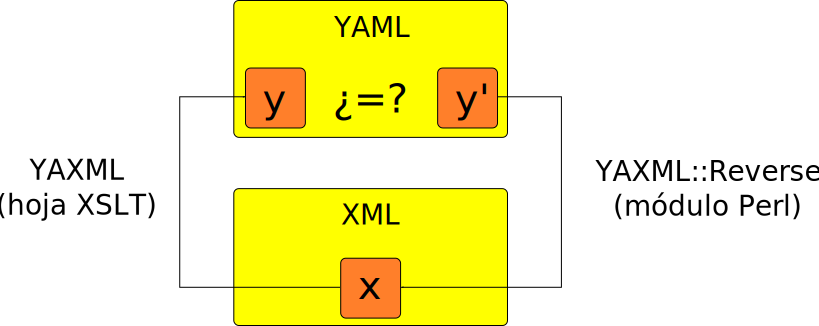
\includegraphics[width=.7\textwidth]{desarrollo/diseno/oraculo_yaxml}
  \caption{Or�culo de pruebas para \nombreyaxml{}}
  \label{fig:oraculo_yaxml}
\end{figure}

\subsubsection{Limitaciones de Perl frente a \acs{YAML}}
\label{sec:limitaciones}

\ac{YAML} se caracteriza por ser una especificaci�n muy flexible,
pudiendo combinar los tipos b�sicos de nodos y etiquetas de muchas
formas. Este fragmento de la especificaci�n~\cite{YAML}, que describe
a los nodos de vector asociativo, es particularmente interesante:

\begin{quotation}
  The content of a mapping node is an unordered set of key: value node
  pairs, with the restriction that each of the keys is unique. YAML
  places no further restrictions on the nodes. In particular, keys may
  be arbitrary nodes, the same node may be used as the value of
  several key: value pairs, and a mapping could even contain itself as
  a key or a value (directly or indirectly).
\end{quotation}

Como vemos, podemos tener claves no escalares e incluso referencias
c�clicas de un mapa como clave de uno de sus elementos. El problema de
los ciclos ya ha sido superado gracias a las anclas y alias, pero usar
claves no escalares es m�s dif�cil de resolver: los vectores
asociativos de Perl, usados como estructura de datos nativa por
\modulo{YAML::XS}, no admiten claves no escalares.

Existen m�dulos como \modulo{Tie::RefHash} que permiten usar clases
que implementan vectores asociativos con claves escalares y no
escalares como si fueran vectores asociativos normales, pero no los
reemplaza directamente, sino que modifica la forma en que Perl eval�a
el c�digo que usa el identificador de la variable ``sobrecargada''. Es
una t�cnica de bajo nivel: no podemos pasar ese vector asociativo y
usarlo en una subrutina como de costumbre, por ejemplo. Adem�s, y lo
que es m�s grave, no nos sirve una vez \modulo{YAML::XS} ha terminado
su procesado: tendr�a que usarse antes de asignarle cualquier
elemento.

Si us�ramos los diccionarios de Python, por ejemplo, uno podr�a
imaginarse emular claves basadas en nodos secuencia mediante tuplas, y
claves basadas en nodos de vector asociativo usando tuplas de
tuplas. Python no permite usar listas ni diccionarios como claves. Sin
embargo, al igual que en el caso de Perl, todo depender�a del
\emph{binding} que estuvi�ramos usando en ese momento.

De todas formas, examinando los lenguajes basados en \ac{YAML}
disponibles actualmente, no parece ser una restricci�n importante: a�n
no he podido encontrar un solo formato basado en \ac{YAML} que tenga
claves no escalares. \ac{JSON} sencillamente no tiene este problema.

Por ello, por lo pronto esta restricci�n se considera de baja
prioridad: solventarla requerir�a la reescritura completa de \yaxml{}
bajo otro entorno (seguramente una aplicaci�n escrita en C, \CPP o
Python), y no supondr�a realmente una ventaja para su uso general.

%%% Local Variables: 
%%% mode: latex
%%% TeX-master: "../../memoria"
%%% End: 

 
\subsection{Capa de aplicaci�n}
\label{sec:capa_aplicacion}
%%
%% Dise�o de la capa de aplicaci�n
%% Copyright (C) 2008 Antonio Garc�a Dom�nguez
%% $Id: capa_aplicacion.tex 622 2008-07-02 09:46:47Z antonio $
%%

La capa de aplicaci�n se ocupa de implementar las clases del modelo de
la arquitectura \ac{MVP}, y de proveer servicios de alto nivel
independientes de la interfaz gr�fica. Esto permite tener separados
todos los aspectos de la interfaz gr�fica respecto de aquellos
relacionados con la l�gica b�sica de \visor{}.

Veremos a continuaci�n cu�les son esas clases del modelo y servicios
ofrecidos, y qu� dise�o siguen.

%% Cambio de un enfoque basado en patrones a un enfoque en
%% componentes: no es cuesti�n de decir "mira, usamos patrones", sino
%% "este componente, por estas razones, ha requerido este patr�n, con
%% estos ajustes"

\subsubsection{Modelos de documentos}

% ModeloDocumento (comparar con ModeloPresentaci�nDocumento)

El concepto fundamental en \visor{} es el de un \clase{Documento}
\ac{XML} abierto por el usuario y preprocesado. Esta clase se ocupa de
encapsular toda esa informaci�n y gestionar los cambios en la hoja de
preprocesado utilizada y la realizaci�n de b�squedas.

N�tese que no se ocupa de la hoja de visualizaci�n: como detalle de
presentaci�n de que se trata, este aspecto se gestiona en su modelo de
presentaci�n, que veremos en \S\ref{sec:capa_presentacion_docs}
(p�gina~\pageref{sec:capa_presentacion_docs}).

Este modelo de documento integra los predicados de b�squedas mediante
palabra completa e ignorando min�sculas definidos mediante extensiones
XPath, dejando a las capas superiores �nicamente la responsabilidad de
definir las \clase{PeticionBusqueda} necesarias.

El conjunto de todas las clases empleadas, tanto del J2SE como de
\visor{}, se halla en el cuadro~\ref{fig:apl_docs}
(p�gina~\pageref{fig:apl_docs}).

\begin{figure}
  \centering
  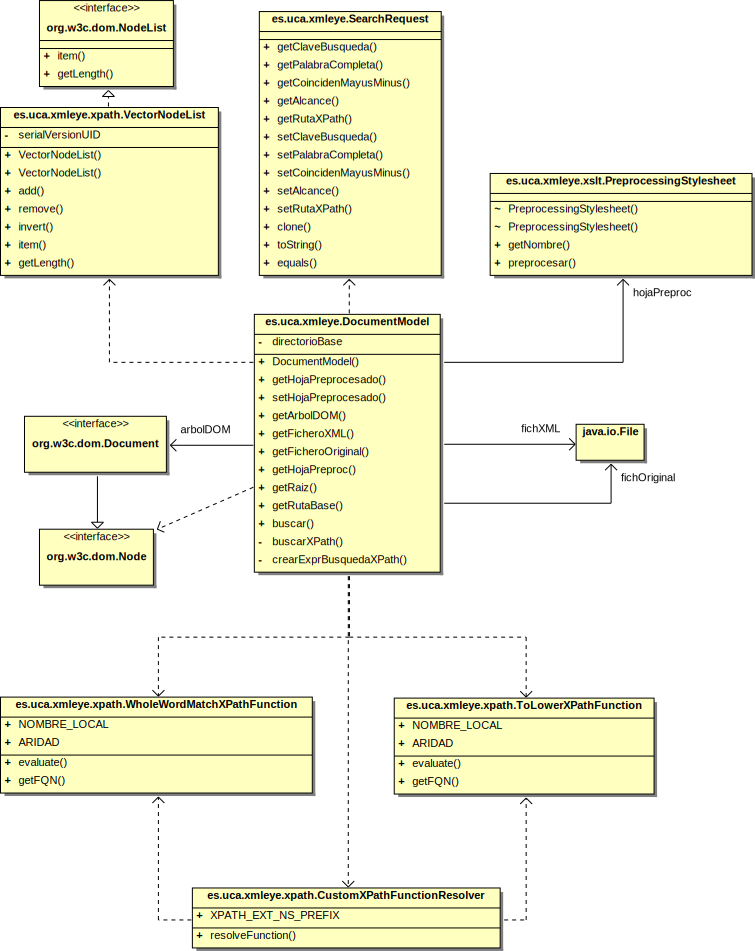
\includegraphics[width=\textwidth]{desarrollo/diseno/clases_xmleye_apl_documentos}
  \caption{Diagrama de clases de dise�o para modelado de documentos}
  \label{fig:apl_docs}
\end{figure}

\subsubsection{Hojas de estilos}

Las hojas de estilos participan tanto en la capa de presentaci�n como
en la capa de aplicaci�n. En la capa de aplicaci�n se halla toda la
infraestructura necesaria para su ejecuci�n, atendiendo a su
estructuraci�n en repositorios y soporte para localizaci�n, en
combinaci�n con el uso de herencia entre distintas hojas. Las propias
hojas son parte de la capa de presentaci�n.

Distinguiremos entre:

\begin{description}
\item[Hoja de usuario] 
  \index{hoja de usuario!definici�n}
  \index{hoja de usuario!punto de acceso}
  \index{hoja de usuario!preprocesado}
  \index{hoja de usuario!visualizaci�n}

  Conjunto cohesivo de una o m�s hojas \ac{XSLT} individuales
  seleccionable por el usuario que conforma un modo de preprocesar el
  documento o visualizar un nodo.

  Se distinguen dos tipos:
  \begin{description}
  \item[Preprocesado]
    Contienen transformaciones que afectan al documento \ac{XML}
    completo tras su apertura. Se usan para modificar el �rbol del
    documento o para realizar operaciones costosas como el
    establecimiento de enlaces.

  \item[Visualizaci�n] Contienen transformaciones a ejecutar sobre el
    nodo \ac{DOM} seleccionado por el usuario en cada momento.
  \end{description}

  Toda hoja de usuario contiene una o varias hojas \ac{XSLT}
  especiales cuyo nombre de fichero sigue el patr�n \fichero{(nombre
    hoja)[idioma[\_pa�s]].xsl}, donde [] indica una parte opcional y
  () una parte obligatoria. Llamamos a dichas hojas sus \emph{puntos
    de acceso}. Se intentar� antes acceder a los puntos de acceso m�s
  espec�ficos respecto del pa�s e idioma de la localizaci�n actual.

\item[Hoja \ac{XSLT}] Fichero individual que contiene un documento
  \ac{XML} definido sobre el vocabulario \ac{W3C} \ac{XSLT}.

\end{description}

Las hojas de usuario han de organizarse cumpliendo una serie de
requisitos:

\begin{itemize}
\item Han de poder ser f�cilmente localizables seg�n el pa�s y el
  idioma de la localizaci�n establecida por el usuario por defecto en
  su sistema.

\item Han de ser f�ciles de instalar, sin requerir configuraci�n
  alguna.

\item Han de ser f�ciles de elaborar, pudiendo basarnos en hojas de
  usuario ya existentes.
\end{itemize}

Los detalles de implementaci�n de cada tipo de hoja de usuario y
aquellos comunes a toda hoja de usuario han sido encapsulados en
clases, permitiendo a la capa de presentaci�n realizar
transformaciones sin conocer los detalles de la biblioteca \ac{XSLT}
usada.

En cuanto a los requisitos sobre la organizaci�n de las hojas de
usuario, se ha mantenido la separaci�n de responsabilidades moviendo
estos requisitos a una clase que act�a de \emph{repositorio}, que se
ocupa de localizar las hojas de usuario y configurarlas para conseguir
al mismo tiempo la capacidad de reutilizar c�digo y localizar las
hojas. La carga del repositorio se realiza al iniciar \visor{}.

La organizaci�n general de las clases utilizadas se halla en la
figura~\ref{fig:apl_hojasusuario} de la p�gina~\pageref{fig:apl_hojasusuario}.

\paragraph{Organizaci�n del repositorio}

El esquema de almacenamiento del repositorio no es configurable,
siendo as� posiblemente menos flexible, pero muy sencillo de
utilizar. La organizaci�n de las hojas de usuario se explica mejor con
un ejemplo. Una posible distribuci�n de hojas \ac{XSLT} de una
hipot�tica hoja de usuario de visualizaci�n llamada \fichero{perso}
bajo el directorio base con la ruta relativa \fichero{xslt} ser�a:

\begin{itemize}
\item \fichero{xslt/view/perso/perso.xsl}: punto de acceso inicial
  para la localizaci�n por omisi�n.
\item \fichero{xslt/view/perso/perso\_en.xsl}: punto de acceso inicial
  para la localizaci�n inglesa, sin especificar el pa�s.
\item \fichero{xslt/view/perso/perso\_en\_GB.xsl}: punto de acceso
  inicial para la localizaci�n inglesa en el Reino Unido.
\item \fichero{xslt/view/perso/logica.xsl}: hoja complementaria que
  permite que los tres idiomas compartan la misma l�gica.
\end{itemize}

Si fuera una hoja de preprocesamiento, se usar�a \fichero{preproc} en
vez de \fichero{view}.

\paragraph{Extensibilidad}
\label{sec:cod_xsl_acceso}

Las hojas de usuario son importadas por la hoja principal no
modificable de su tipo, en la ra�z del repositorio, que define la
m�nima funcionalidad com�n: \fichero{view.xsl} para las hojas de
visualizaci�n y \fichero{preproc.xsl} para las de preprocesado.

Adem�s, una hoja de usuario puede importar a otras y as�
especializarlas. Es el caso de \fichero{ppACL2}, que importa a
\fichero{xml}.

Para abstraer a las hojas de la l�gica de internacionalizaci�n, una
hoja de usuario que desee importar a otra puede usar \ac{URI}
especiales como \texttt{view\_ppACL2}. 

Mediante esta \ac{URI}, se acceder� a la hoja de usuario de
visualizaci�n \fichero{ppACL2} a trav�s del punto de acceso que mejor
se ajuste a la localizaci�n actual del usuario.

\paragraph{Internacionalizaci�n}
\label{sec:cod_xsl_l10n}

El ejemplo de \fichero{perso} anterior ilustra el mecanismo de
localizaci�n establecido por la l�gica de la capa de aplicaci�n. Dicho
mecanismo imita al usado por los \clase{ResourceBundle}s de la
biblioteca est�ndar de Java.

Si la localizaci�n  actual por defecto es ``es\_ES'' (espa�ol, Espa�a) y se
busca la hoja de visualizaci�n \fichero{ppACL2},
\clase{ControlHojasXSL} intentar� localizar un punto de acceso en el
siguiente orden:
\begin{enumerate}
\item \fichero{xslt/view/ppACL2/ppACL2\_es\_ES.xsl}
\item \fichero{xslt/view/ppACL2/ppACL2\_es.xsl}
\item \fichero{xslt/view/ppACL2/ppACL2.xsl}
\end{enumerate}

\begin{figure}
  \centering
  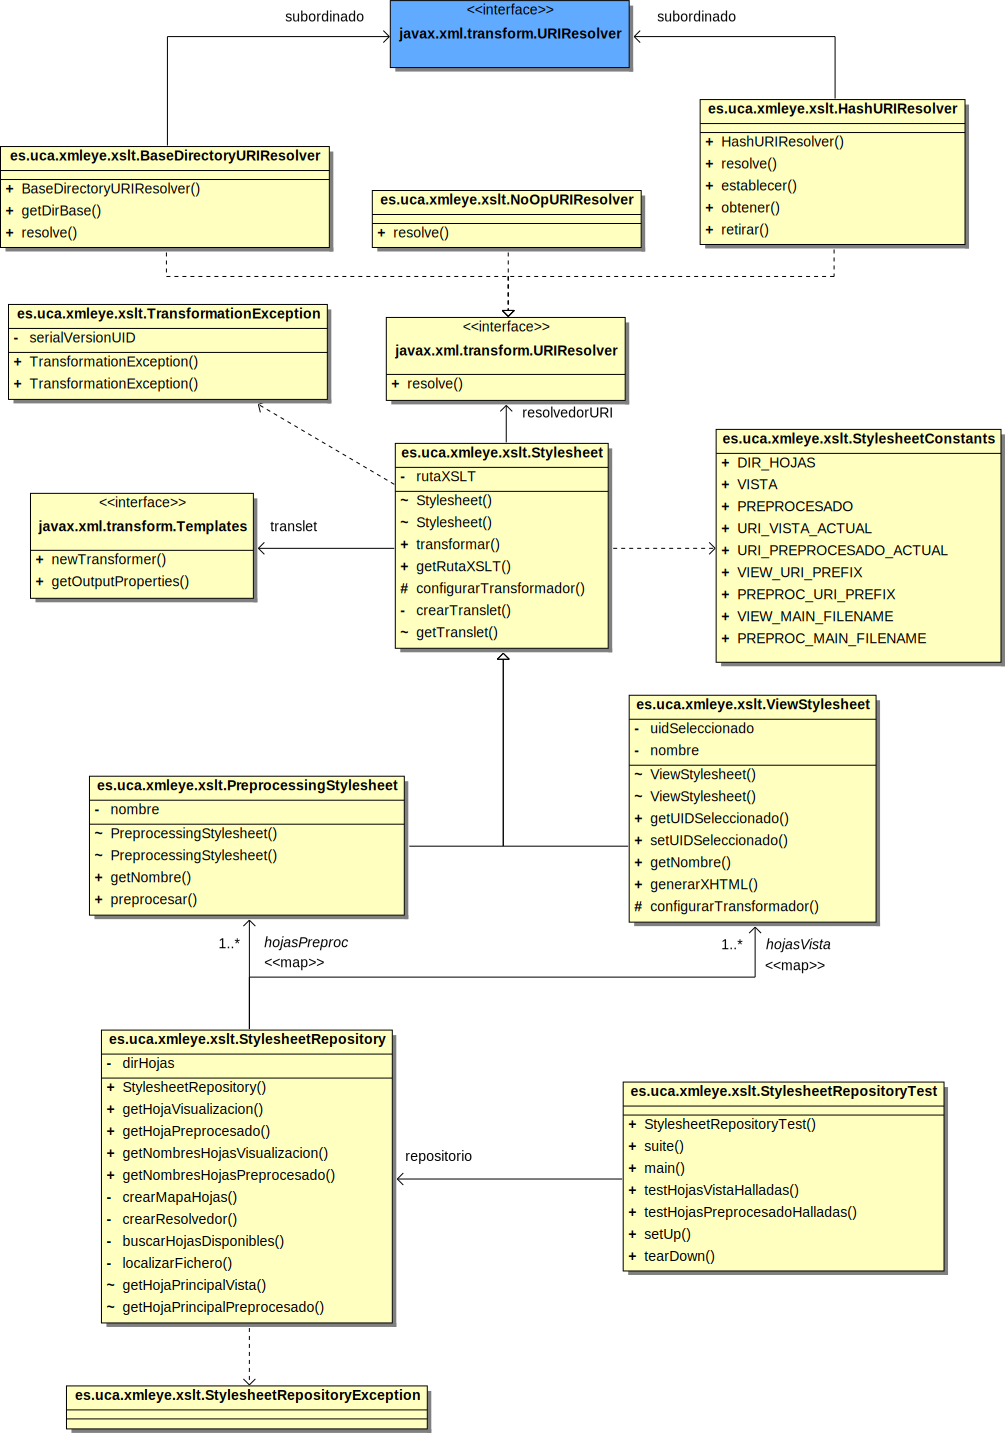
\includegraphics[width=.9\textwidth]{desarrollo/diseno/clases_xmleye_apl_hojas}
  \caption{Diagrama de clases de dise�o para las hojas de usuario}
  \label{fig:apl_hojasusuario}
\end{figure}

\subsubsection{Descriptores de formatos}

Otro servicio tambi�n a prestar por la capa de aplicaci�n es el de la
gesti�n de los descriptores de formatos de documento. Al igual que en
el caso de las hojas, se necesitaba abstraer a las capas superiores de
los detalles de un descriptor individual y de la forma en que se
hallan organizados.

Volvemos a tener otro repositorio, esta vez de descriptores, en el que
se siguen una serie de convenciones para evitar la necesidad de
realizar cualquier tipo de configuraci�n. A diferencia del repositorio
de hojas, no tratamos con un �nico �rbol de directorios: se pueden
encadenar varios, y as� poder tener una serie de ajustes a nivel
global para todos los usuarios, y otros locales para el usuario
actual. Para restaurar los ajustes locales a los globales, s�lo hemos
de borrar el descriptor a nivel local y actualizarlos.

\index{patr�n de dise�o!Observador}
\index{Singleton|see{patr�n de dise�o!Observador}}

Este repositorio abstrae tambi�n la l�gica que hace corresponder un
descriptor a un fichero determinado, y se ocupa de validar contra un
XML Schema todos los descriptores. El repositorio es un
\clase{AbstractListModel} de Swing, por lo que puede integrarse
f�cilmente como modelo de un formulario e incluso registrar
\patron{Observador}es sobre �l si se estima necesario, pero no es obligatorio.

Por otro lado, las clases para los descriptores individuales
encapsulan el formato de estos ficheros y proporcionan toda la
validaci�n necesaria de su contenido, lanzando excepciones cuando se
intentan establecer valores no v�lidos en alg�n atributo.

Las clases implicadas se hallan en el
cuadro~\ref{fig:aplicacion_formatos} de la
p�gina~\pageref{fig:aplicacion_formatos}.

\begin{figure}
  \centering
  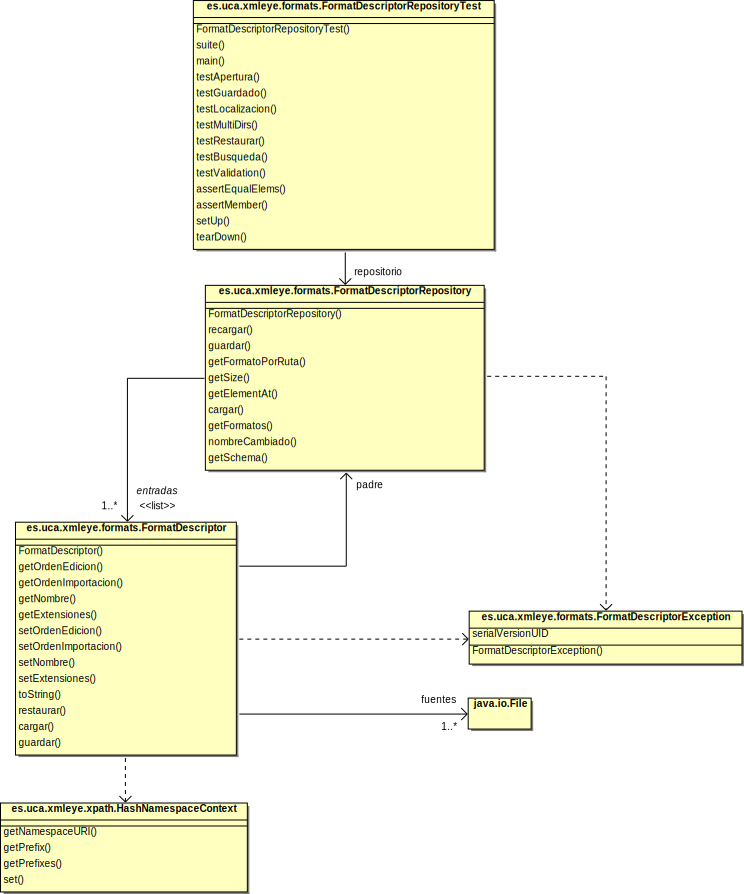
\includegraphics[width=\textwidth]{desarrollo/diseno/clases_xmleye_apl_descriptores}
  \caption{Diagrama de dise�o de clases de descriptores de formatos}
  \label{fig:aplicacion_formatos}
\end{figure}

% , descriptores de formatos (detalles
% de almacenamiento multinivel en repositorio, abstracci�n de los
% ficheros en forma de objetos, localizaci�n, restauraci�n)

\subsubsection{Notificaci�n de cambios sobre ficheros}

\index{patr�n de dise�o!Observador}
\index{Singleton|see{patr�n de dise�o!Observador}}

Un requisito muy interesante era el de poder vigilar los cambios
realizados sobre los documentos durante su visualizaci�n, pudiendo
mantener el editor y \visor{} abiertos en paralelo. Para ello se ha
implementado una clase que ofrece una interfaz basada en el patr�n
Observador, que se basa en la fecha de modificaci�n para notificar de
cambios en los contenidos del fichero.

Para ello, se usa un hilo en segundo plano de baja prioridad, que se
despierta cada cierto tiempo, realiza la comprobaci�n y vuelve a
dormir. Esto evita la p�rdida de rendimiento que supondr�a un bucle de
espera activa. Adem�s, las actualizaciones pueden pausarse y
reactivarse a voluntad.

% Observador

\subsubsection{Persistencia de preferencias}

% Singleton (�nicamente como punto de acceso, permite cambio backend en un futuro)

\label{sec:aplic_singleton}
\index{patr�n de dise�o!Inyecci�n de Dependencias}
\index{patr�n de dise�o!Singleton}
\index{Inyecci�n de Dependencias|see{patr�n de dise�o!Inyecci�n de Dependencias}}
\index{Singleton|see{patr�n de dise�o!Singleton}}

En este caso es fundamental tener un punto de acceso central a todas
las preferencias de los usuarios. Por estas razones, en la versi�n
original del visor se utiliz� el patr�n \patron{Singleton}, asegurando
la existencia de una �nica instancia de una clase que implementara una
interfaz. Se utiliz� una versi�n mejorada de la implementaci�n usual
tomada de~\cite{gof}, simplificando sobre la sugerida
en~\cite{singletonjava}.

Sin embargo, durante el desarrollo de esta nueva versi�n, se vio que
el uso del Singleton dificultar�a la posterior realizaci�n de pruebas
con sustitutos, e introduc�a una dependencia innecesaria. 

Para retirarla, se aplic� el patr�n \patron{Inyecci�n de
  Dependencias}: ahora no son las clases las que solicitan el gestor
de preferencias, sino las que lo reciben a trav�s de su
constructor. De esta forma, no se necesita el punto �nico de acceso
como antes, siendo muy f�cilmente sustituible durante pruebas, por
ejemplo, y manteniendo la independencia respecto a la implementaci�n a
trav�s del uso de una interfaz.

El diagrama de las clases involucradas en la gesti�n de preferencias
se halla en el cuadro~\ref{fig:dc_aplic_prefs} de la
p�gina~\pageref{fig:dc_aplic_prefs}. Podemos ver que el
\patron{Singleton} ha desaparecido, al ser ahora completamente
innecesario.

Se dispone de un valor booleano almacenado directamente en
dependencias, de tal forma que una clase que requiera un atributo con
persistencia entre las preferencias s�lo tendr� que instanciar
apropiadamente esta clase y luego utilizar \lstinline{get()} y
\lstinline{set()} sin m�s complicaciones.

%% sigue igual, pero cuidado con las fachadas

En el diagrama de secuencia~\ref{fig:ds_aplic_prefs} de la
p�gina~\pageref{fig:ds_aplic_prefs} puede verse c�mo se gestionan
las preferencias a lo largo del programa:
\begin{itemize}
\item Al iniciarse \visor{}, se crea una instancia de la clase
  principal que representa a toda la aplicaci�n. Esta clase es la
  ocupada de ensamblar a todas las dem�s clases de mayor nivel,
  inyectando las dependencias consideradas oportunas y evitando que
  dependan demasiado entre s�.

\item La clase principal ensambladora crea una instancia de la
  implementaci�n de gesti�n de preferencias a usar, y solicita que se
  carguen las preferencias.

\item La clase principal ensambla el modelo de presentaci�n de la
  ventana principal con el gestor de preferencias (visto a trav�s de
  su interfaz) y otros par�metros. Tambi�n ensambla y lanza la ventana
  principal.

\item Al cerrar la aplicaci�n, la misma clase principal solicita el
  guardado de las preferencias antes de terminar la ejecuci�n del
  programa.

\end{itemize}

\begin{figure}
  \centering
  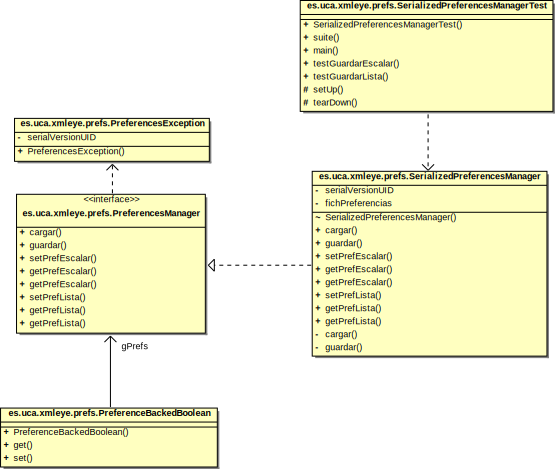
\includegraphics[width=\textwidth]{desarrollo/diseno/clases_xmleye_apl_prefs}
  \caption{Diagrama de clases de dise�o de gesti�n de preferencias}
  \label{fig:dc_aplic_prefs}
\end{figure}

\begin{figure}
  \centering
  \includegraphics[width=\textwidth]{desarrollo/diseno/diag_sec_xmleye_prefs}
  \caption{Diagrama de secuencia de gesti�n de preferencias}
  \label{fig:ds_aplic_prefs}
\end{figure}

%%% Local Variables: 
%%% mode: latex
%%% TeX-master: "../../memoria"
%%% End: 

 
\subsection{Capa de presentaci�n}
\label{sec:capa_presentacion}
%%
%% Dise�o de la capa de presentaci�n
%% Copyright (C) 2009 Antonio Garc�a Dom�nguez
%% $Id: capa_presentacion.tex 621 2008-07-02 09:04:44Z antonio $
%%

%% Organizaci�n general de la interfaz
%
% - cada documento tiene su modelo de presentaci�n, conectado al de la
% ventana principal.
%
% - ventana principal tiene su modelo de presentaci�n.
%
% - ventana de formatos tiene su modelo, usado por la ventana
% principal, pero sin conocimiento del modelo de presentaci�n de
% formatos
%
% - ventanas "acerca de" y "buscar" _no_ tienen modelos de
% presentaci�n, al ser muy simples. Ventana de Buscar se comunica con
% la principal a trav�s de un patr�n Observador, evitando que est�
% acoplada al modelo de presentaci�n completo. Ventana "Acerca de" es
% pr�cticamente un di�logo est�tico, por lo que no hay nada de
% interesante en su dise�o.
% 
% - vistas (DocumentView, DocumentList, WndMain, etc.) sincronizan por
% su cuenta con los modelos de presentaci�n, evitando complicar estos
% con los detalles de los controles GUI usados, y mejorando la
% capacidad para hacer pruebas respecto a la versi�n anterior.
%%

La capa de presentaci�n se encarga de la comunicaci�n persona-m�quina,
realizando peticiones sobre la capa de aplicaci�n y mostrando los
resultados.

Durante el dise�o de la interfaz, se usaron las
obras~\cite{jlfguid,jlfguidadv} como gu�a, como en el caso del dise�o
del di�logo ``Buscar'', donde el reparto de los componentes sigue sus
recomendaciones. Otras recomendaciones seguidas son la ejecuci�n de
las tareas largas en segundo plano, los elementos de los que deben
constar los men�s, o las combinaciones de teclas recomendadas para
cada opci�n.

\subsubsection{Estructura general}
\label{sec:capa_presentacion_general}

\index{patr�n arquitect�nico!MVP}
\index{patr�n arquitect�nico!Modelo de Presentaci�n}

Como ya se coment� en \S~\ref{sec:arquitectura_mvp}
(p�gina~\pageref{sec:arquitectura_mvp}), la capa de presentaci�n se
ocupar�a de los elementos Vista y Presentaci�n del tr�o
Modelo-Vista-Presentaci�n. En particular, se utilizar�a la variante
\patron{Modelo de Presentaci�n}, que nos permite definir la l�gica de
una forma completamente separada de la interfaz, y as� poder crear
nuevas interfaces de manera mucho m�s libre.

\visor{} dispone b�sicamente de 4 formularios, tal y como se
estableci� durante el an�lisis (apartado~\ref{sec:req_externas} en la
p�gina~\pageref{sec:req_externas}): el formulario principal, el
formulario de gesti�n de descriptores de formatos, el formulario de
realizaci�n de b�squedas, y por �ltimo el formulario con informaci�n
acerca de \visor{}.

Descartando el �ltimo de este apartado por su sencillez, podemos ver
que el formulario principal y el de gesti�n de formatos son los m�s
complejos. Por ello, modelaremos su estado con \patron{Modelos de
  Presentaci�n}, permitiendo una mejor comprensi�n y depuraci�n de su
c�digo. El formulario de b�squeda es m�s sencillo, y por lo tanto no
requiere dicho enfoque, como veremos posteriormente.

Adem�s de los modelos de presentaci�n, hablaremos en el resto de esta
secci�n de otros aspectos interesantes del dise�o de la capa de
presentaci�n.

\subsubsection{Modelos de presentaci�n y su ensamblaje}
\label{sec:capa_presentacion_docs}

\index{patr�n de dise�o!Observador}
\index{patr�n de dise�o!MVP}
\index{patr�n de dise�o!Inyecci�n de Dependencias}

En los formularios m�s complejos, se pudo ver r�pidamente que el uso
del patr�n \patron{Observador} para aspectos como el control de hojas
usadas y dem�s hac�a el c�digo cada vez m�s dif�cil de estructurar y
depurar. Adem�s, este c�digo imped�a poder aislar de manera efectiva
el estado de m�ltiples documentos.

Por ello, se cambi� a un enfoque donde unas clases encapsulan el
estado de la interfaz, de forma independiente a los controles
Swing. Estas clases ofrecen una serie de m�todos \metodo{get} p�blicos
para acceder al estado de la interfaz, y disponen tambi�n de un m�todo
por cada gesto de inter�s que pueda provenir del usuario.

Las vistas se reducen, por lo tanto, a informar de los gestos del
usuario al modelo de presentaci�n y posteriormente sincronizarse con
los modelos. Al quedarse sin la mayor parte de su l�gica, el hecho de
no poder realizar pruebas sobre los propios controles Swing no es tan
importante: podemos hacer pruebas sobre el modelo de presentaci�n,
enviando los gestos y estudiando su estado posterior.

Los modelos de presentaci�n pueden anidarse: as�, el modelo de
presentaci�n del formulario principal contiene a los modelos de
presentaci�n de cada documento, que contienen a su vez a los modelos
(ya no de presentaci�n) de los documentos correspondiente, junto con
otros elementos como una referencia al repositorio de hojas o al
repositorio de descriptores de formato. Entre los campos de todo
modelo de presentaci�n se encuentra el nodo seleccionado actualmente,
la hoja de visualizaci�n que est� siendo usada o la �ltima b�squeda
realizada, por ejemplo.

Los modelos de presentaci�n dependen de otros objetos, como ya hemos
visto, pero no deber�an quedarse acoplados a una implementaci�n o
instancia particular de ellos. En su lugar, estas dependencias se
proporcionan a trav�s del constructor, constituyendo una
\patron{Inyecci�n de Dependencias}. Los modelos de presentaci�n y sus
dependencias y la vista del formulario principal son creados y
configurados por un ensamblador central: la clase principal de la
aplicaci�n. Esto asegura que toda la l�gica relevante se halle en un
�nico sitio, y el resto de las clases se mantengan lo m�s flexibles
posible.

El diagrama de clases que describe las relaciones entre las distintas
vistas principales (formularios, listas de pesta�as y pesta�as) y los
modelos de presentaci�n se halla en el
cuadro~\ref{fig:presentacion_modpre} de la
p�gina~\pageref{fig:presentacion_modpre}.

\begin{figure}
  \centering
  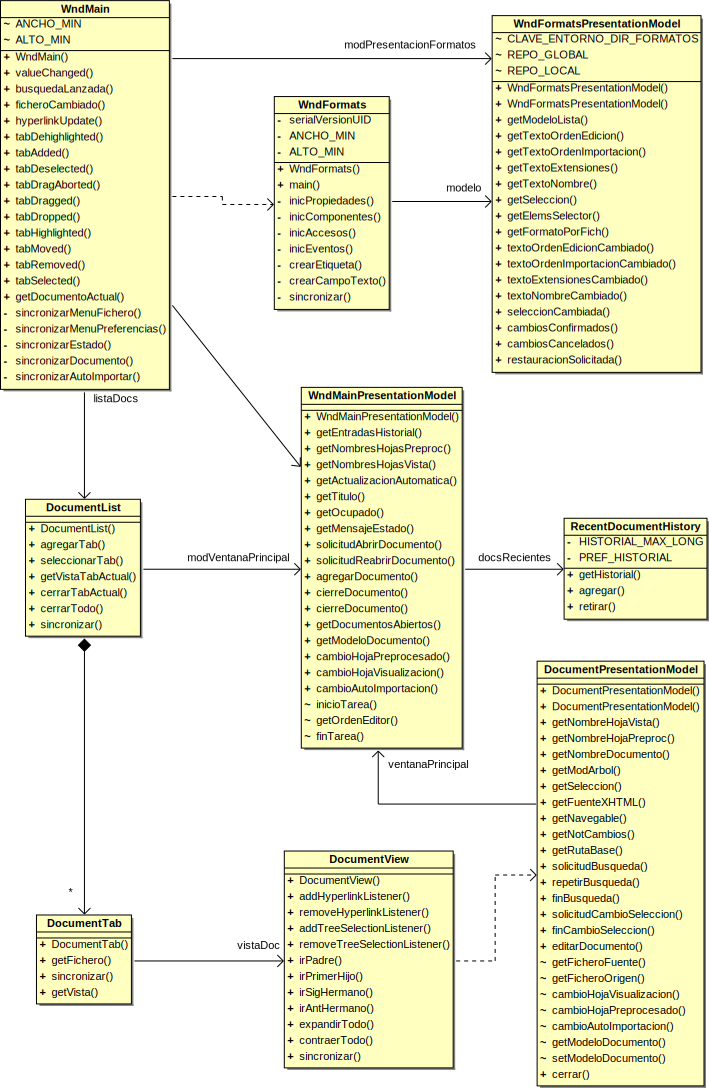
\includegraphics[width=.9\textwidth]{desarrollo/diseno/clases_xmleye_pre_modelos}
  \caption{Diagrama de clases de dise�o de los modelos de presentaci�n}
  \label{fig:presentacion_modpre}
\end{figure}

\subsubsection{Dise�o e integraci�n del formulario de b�squeda}

% Patr�n Observador

\index{patr�n arquitect�nico!Observador}

El formulario de b�squeda es una excepci�n al uso del patr�n
\ac{MVP}. Este di�logo carece pr�cticamente de l�gica propia, siendo
�nicamente una interfaz a partir de la cual el usuario puede construir
la petici�n de b�squeda y enviarla a sus suscriptores, entre los
cuales se halla el modelo de presentaci�n del formulario principal.

Aplicando de esta forma el patr�n \patron{Observador}, se evita el
acoplamiento del formulario de b�squeda al formulario principal, y se
puede guardar el evento para posteriormente repetir la b�squeda sin
necesidad de volver a mostrarlo, por ejemplo.

El formulario principal, como es com�n, se limita a notificar del
gesto al modelo de presentaci�n, que utiliza la funcionalidad del
modelo del documento para implementar la b�squeda, a�adiendo algo m�s
de inteligencia en lo que respecta a b�squedas repetidas.

Puede verse el diagrama de clases de dise�o correspondiente en el
cuadro~\ref{fig:presentacion_busq} de la p�gina~\pageref{fig:presentacion_busq}.

\begin{figure}
  \centering
  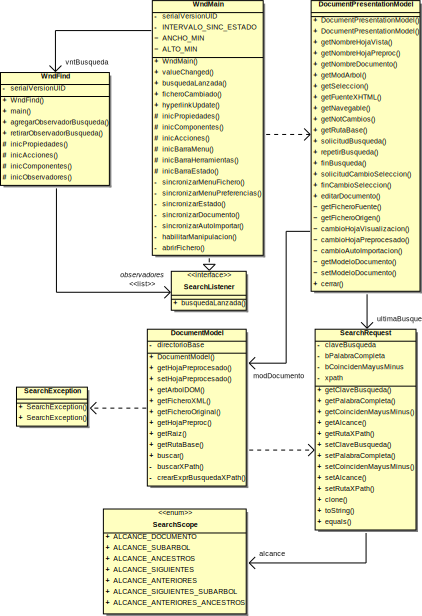
\includegraphics[width=.9\textwidth]{desarrollo/diseno/clases_xmleye_pre_busqueda}
  \caption{Diagrama de clases de dise�o de b�squedas}
  \label{fig:presentacion_busq}
\end{figure}

\subsubsection{Gesti�n de di�logos de mensajes}
\label{sec:presentacion_mensajes}

\index{patr�n arquitect�nico!Singleton}

%% SI: pero la necesidad viene de refactorizar en una clase com�n
%% informes de errores que vengan de otros hilos que no sean el de la
%% interfaz Swing, y de usar el patr�n Singleton para evitar tener que
%% usar m�todos est�ticos, que restar�an flexibilidad para el futuro.

A diferencia del caso de~\S\ref{sec:aplic_singleton}, se ha mantenido
el uso del patr�n \patron{Singleton} para la gesti�n de di�logos de
mensaje: el punto de acceso global en este caso es realmente
necesario, y la l�gica que provee es muy concreta.

En particular, la clase a la que da acceso el \patron{Singleton}
permite mostrar esos di�logos de forma independiente al hilo en que
nos hallemos: normalmente, para poder lanzar un di�logo debemos
hacerlo en el hilo de Swing, o se crear�n condiciones de carrera
indeseadas. Esta clase hace uso de las \clase{SwingUtilities} para
enviar las tareas apropiadas al hilo de Swing desde cualquier otro de
los hilos, como cuando estamos convirtiendo un documento de entrada,
por ejemplo.

Sin embargo, en este caso, no se ha dividido en una interfaz y una
implementaci�n, ya que a diferencia de la gesti�n de preferencias, no
se est�n considerando implementaciones alternativas.

\subsubsection{Presentaci�n de �rboles XML dirigidos por datos}
\label{sec:presentacion_mvc}

\index{patr�n arquitect�nico!MVC}
\index{patr�n arquitect�nico!Documento-Vista}

Los componentes usados para visualizar �rboles \ac{DOM} \ac{XML}
emplean, como todo componente Swing, una modificaci�n~\cite{swingarch}
del patr�n \patron{Modelo-Vista-Controlador} original de~\cite{gof}.

En esta versi�n modificada, llamada ``arquitectura de modelo
separable'' por Sun y similar al patr�n \patron{Documento-Vista} mencionado
en~\cite{archpatterns}, se dividen los componentes en tres partes:
\begin{itemize}
\item El componente Swing que implementa los aspectos de vista y
  controlador.
\item El objeto del Look \& Feel instalado en el componente Swing que
  define el aspecto exacto del componente.
\item El modelo del componente, es decir, la informaci�n que contiene,
  y que modifica su visualizaci�n o comportamiento. En Swing, el
  modelo puede contener tambi�n detalles de la interfaz gr�fica: bot�n
  activado o desactivado, por ejemplo.
\end{itemize}

As�, se han definido dos \clase{TreeModel}:
\begin{description}
\item[\clase{DOMTreeModel}] 

  Modelo sobre un �rbol \ac{DOM} \ac{XML} est�ndar, que hace
  accesibles los nodos de tipo elemento.

\item[\clase{DataDrivenTreeModel}] 

  Especializaci�n del anterior, este modelo incorpora la capacidad de
  realizar falsas podas, ocultando nodos de la visualizaci�n sin
  eliminarlos del �rbol \ac{DOM}.

  La decisi�n de ocultar un nodo o sus hijos se halla en el propio
  documento \ac{XML}. De esta forma, el usuario puede controlar este
  aspecto a trav�s de las hojas \ac{XSLT}, dirigi�ndolo todo por
  datos.

  En los campos \metodo{ATTRIBUTE\_LEAF} y \metodo{ATTRIBUTE\_HIDDEN} de
  \clase{DataDrivenTreeModel} se hallan los atributos que deben
  tomar el valor del campo \metodo{ENABLED\_VALUE} para activar la
  ocultaci�n de los hijos o del propio nodo, respectivamente.
\end{description}

Por las mismas razones que \clase{DataDrivenTreeModel}, se implement�
l�gica de dibujado dirigida por datos de los nodos del \clase{JTree}
mediante la clase \clase{DataDrivenTreeCellRenderer}. Este dibujador
puede modificar el icono y la etiqueta de un nodo a trav�s de sus
propios atributos \metodo{NODELABEL\_ATTRIBUTE} y
\metodo{NODEICON\_ATTRIBUTE}.

Se extendieron las capacidades de \clase{JTree} en \clase{DOMTree},
implementando operaciones para encapsular la navegaci�n por el �rbol y
abstraer al resto de la interfaz de los detalles, como
\metodo{selectParent}.

En la figura~\ref{fig:dc_presentacion_arboles}
(p�gina~\pageref{fig:dc_presentacion_arboles}) se ilustran en un
diagrama \ac{UML} las relaciones entre las clases relacionadas con la
visualizaci�n de �rboles \ac{XML}, incluyendo sus casos de prueba.

\begin{figure}
  \centering
  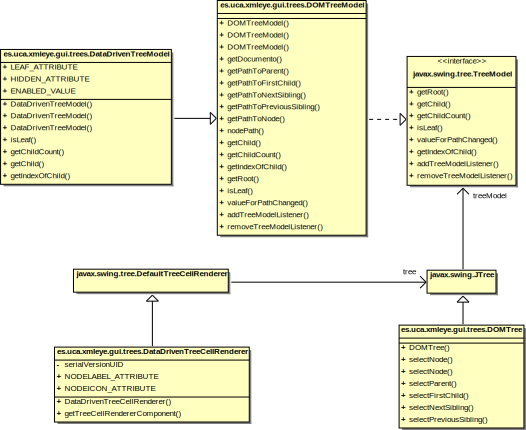
\includegraphics[width=\textwidth]{desarrollo/diseno/clases_xmleye_pre_arboles}
  \caption{Diagrama de clases de manejo de �rboles}
  \label{fig:dc_presentacion_arboles}
\end{figure}

\subsubsection{M�ltiples m�todos de acceso a una acci�n por el usuario}
\label{sec:presentacion_orden}

\index{patr�n arquitect�nico!Orden}

Otro patr�n de dise�o empleado com�nmente en las interfaces gr�ficas
es el patr�n Orden, y esta interfaz no es una excepci�n. 

En este patr�n, se define una interfaz para una acci�n gen�rica. El
lanzador de las acciones recibe objetos que cumplen tal interfaz. Al
generarse el evento de inter�s, reacciona ejecutando cada una de las
acciones a trav�s de dicha interfaz.

Este patr�n permite aislar al elemento que lanza la acci�n del que
realiza la acci�n. As�, podemos asociar cualquier acci�n a un control
Swing, sin que deba saber exactamente qu� hace esa acci�n. S�lo conoce
la interfaz que debe cumplir la acci�n, limit�ndose a invocar al
m�todo correspondiente.

Adem�s de reducir el acoplamiento, tambi�n mejora la estructura del
programa evitando la duplicaci�n de c�digo al codificar la misma
l�gica en varios componentes.

Es el caso usual de las acciones disponibles mediante la barra de
herramientas, un acceso de teclado y un elemento del men�, por
ejemplo: no importa exactamente qui�n lanza el evento, s�lo qu� acci�n
se lanza.

En Swing, la interfaz a cumplir es \clase{Action}, que permite no s�lo
unificar la orden a ejecutar, sino tambi�n parte de su visualizaci�n.
Podemos asignar un acelerador de teclado, una descripci�n corta y un
mnem�nico a una acci�n, y al crear un bot�n o elemento de men� a
partir de ella, �stos se inicializar�n con los valores correctos.


%%% Local Variables: 
%%% mode: latex
%%% TeX-master: "../../memoria"
%%% End: 


%%% Local Variables: 
%%% mode: latex
%%% TeX-master: "../../memoria"
%%% End: 


\section{Implementaci�n}
\label{sec:implementacion}
%%
%% Detalles de implementaci�n interesantes
%% Copyright (C) 2008 Antonio Garc�a Dom�nguez
%% $Id: implementacion.tex 629 2008-07-06 13:47:58Z antonio $
%%

\subsection{Perl}
\label{sec:codificacion_perl}

Se usaron la obra~\cite{perlbyexample} y la web~\cite{perldoc} como
referencias para los aspectos de divisi�n en m�dulos y la
implementaci�n en Perl del paradigma orientado a objetos.

Varios detalles de implementaci�n de ciertos patrones y otras
pr�cticas recomendadas para Perl se obtuvieron de~\cite{perloowiki}.

\lstset{language=Perl}

\subsubsection{Perl y el paradigma OO}
\label{sec:perl_oo}

No hay que confundir el hecho de emplear el paradigma orientado a
objetos con el uso de un lenguaje orientado a objetos.

Perl proporciona mecanismos para implementar la mayor�a de la
funcionalidad necesaria para este paradigma, pero no proporciona un
soporte directo a trav�s del lenguaje de muchas construcciones, como
una sintaxis espec�fica para declaraci�n de clases con palabras
reservadas para control de acceso, por ejemplo.

Otras veces ha de usarse una sintaxis algo m�s compleja de lo usual,
como en el caso de las variables de instancia.

Para implementar los m�todos, por ejemplo, Perl permite ``bendecir''
una referencia cualquiera con el nombre de un m�dulo. A partir de ese
momento, se buscar� la subrutina \metodo{metodo} dentro del m�dulo con
el que se bendijo \verb!$variable! al usar esta sintaxis:
\begin{lstlisting}
 $variable->metodo(@args);
\end{lstlisting}%$

Un m�dulo puede declarar a otros como base, que ser�n consultados
mediante un recorrido primero en profundidad sobre el �rbol de
generalizaciones durante la b�squeda de un m�todo. Este mecanismo es
el que implementa la herencia y los m�todos virtuales.

\subsubsection{Internacionalizaci�n}
\label{sec:cod_perl_l10n}

La internacionalizaci�n de los mensajes se consigue en
\postprocesador{} a trav�s del m�dulo \modulo{Locale::Maketext}, que
permite usar una jerarqu�a de clases donde la clase base define la
l�gica com�n y los idiomas por omisi�n y sus hijas contienen un
diccionario que realiza la localizaci�n para cada idioma (posiblemente
especificando el pa�s).

El uso es muy sencillo:
\begin{lstlisting}[caption=Ejemplo de uso de Locale::Maketext]
# Obtenemos el manejador a la localizaci�n que m�s se ajuste,
# subclase de ACL2::Localizacion, que es a su vez subclase
# de Locale::Maketext.
my $lh = ACL2::Localizacion->get_handle();

# Buscamos en el diccionario y sustituimos
# la cadena original: buscando 'Hola [_1]' se hallar�a 
# 'Hello [_1]' y luego se sustituir�a, dando 'Hello Pablo'.
print $lh->maketext("Hola [_1]", 'Pablo');
\end{lstlisting}

Dicho m�dulo es t�cnicamente superior al conocido \texttt{Gettext},
por la flexibilidad que su enfoque orientado a objetos le aporta: se
pueden definir funciones para manejar las formas plurales seg�n el
lenguaje, por ejemplo, simplemente redefiniendo un m�todo en la clase
correspondiente. 

Tambi�n numera los par�metros de las cadenas, permitiendo mayor
flexibilidad que la usual cadena con par�metros para \metodo{printf},
que da resultados pobres en casos en los que haya que cambiar el orden
de las palabras.

\subsubsection{Distribuci�n mediante \acs{PAR}}

Distribuir \postprocesador{} era bastante complejo e inc�modo en su
anterior versi�n. Se deseaba facilitar este aspecto en la mayor medida
de lo posible, permitiendo instalar de forma autom�tica las
dependencias o empaquetarlas en un formato c�modo de utilizar.

Este problema no es �nico a \postprocesador{}: empezando por \yaxml{},
pr�cticamente todo m�dulo sufre de �l. Existen muchas alternativas,
como \verb#perlcc# (retirado a partir de Perl 5.10), Perl2Exe o
Perl2App, pero entre todas ellas destacan \modulo{PAR} y
\modulo{PAR::Packer}.

De forma muy similar a los ficheros \fichero{.jar} de Java,
\modulo{PAR::Packer} y su herramienta \verb#pp# nos permiten crear
ficheros \fichero{.par} con todo el c�digo fuente de los conversores y
sus dependencias que no forman parte de los m�dulos est�ndar de
Perl. 

Instalar estos conversores y sus hojas se convierte en algo tan
sencillo como descargar el \fichero{.par} correspondiente a nuestra
plataforma y descomprimirlo sobre el directorio ra�z de
XMLEye. Adem�s, si nuestra aplicaci�n es Perl puro, el \fichero{.par}
generado puede ser usado en cualquier arquitectura y sistema
operativo.

Si no queremos obligar a nuestros usuarios a tener que instalar un
entorno Perl y los m�dulos \modulo{PAR} y \modulo{PAR::Packer} (cosa
particularmente molesta en Windows), tambi�n podemos crear ejecutables
monol�ticos, espec�ficos del sistema operativo y arquitectura bajo el
que se creen, que incluyen hasta el propio int�rprete de Perl con sus
m�dulos est�ndar.

Estas im�genes no son tan grandes como se esperar�a: los
\fichero{.par} para \yaxml{} y \postprocesador{} no llegan a los
100KiB, y los ejecutables, una vez comprimidos, no alcanzan los
2MiB. Adem�s, estas distribuciones comprimidas incluyen todos los
descriptores de formato y hojas de usuario necesarias.

\subsection{Java}
\label{sec:cod_java}

\lstset{language=Java}

Un texto �til ha sido la referencia del lenguaje~\cite{javalang},
escrita por los creadores de Java. La web~\cite{swingwiki} detalla
adem�s algunas pr�cticas recomendadas, funcionalidades no documentadas
y soluciones temporales a fallos conocidos de Swing.

Un ejemplo es la disponibilidad no documentada de fuentes con
anti-aliasing bajo la \ac{J2SE} 5.0, o la necesidad de forzar
manualmente un tama�o m�nimo sobre los hijos de \clase{JFrame}, un
fallo documentado en la propia base de datos de Sun y corregido en la
pr�xima \ac{J2SE} 6.0 ``Mustang''.

El uso del \ac{IDE} Eclipse 3.3.2 ha sido fundamental gracias a su
soporte para la realizaci�n sencilla de refactorizaciones a gran
escala, pudiendo renombrar m�todos y clases completas sin introducir
errores en el c�digo, entre otras cosas.

\subsubsection{Controles HTML}
\label{sec:cod_java_html}

Los controles para navegaci�n \ac{HTML} incluidos en Swing dejan
bastante que desear a la hora de usar el teclado para navegar o
seleccionar enlaces.

Para cubrir estas carencias, se especializ� la clase
\clase{JEditorPane} en \clase{Browser}.

Otros componentes �tiles incluyen un observador de enlaces capaz de
lanzar uno de los navegadores web del usuario (el navegador por
defecto en Windows y Mac OS X) al pulsar enlaces con \acs{URL}
v�lidas.

\subsubsection{Internacionalizaci�n}
\label{sec:cod_java_l10n}

En el lado de Java, la internacionalizaci�n se obtiene a partir de los
\clase{ResourceBundle}s, de los que hay dos tipos:
\begin{itemize}
\item \clase{PropertyResourceBundle}s, que acceden a ficheros
  \fichero{.properties} de f�cil mantenimiento, al s�lo contener
  cadenas de texto.
\item Especializaciones de \clase{ListResourceBundle}, que pueden
  contener cualquier tipo de objeto.
\end{itemize}

La capa de aplicaci�n s�lo maneja mensajes de texto y usa el primer
tipo, y la capa de presentaci�n usa el segundo tipo, al necesitar
adem�s iconos y atajos de teclado.

La clase \clase{ResourceBundle} de la biblioteca est�ndar de Java es
la ocupada de hallar e instanciar el \clase{PropertyResourceBundle} o
\clase{ListResourceBundle} que se ajuste mejor a la localizaci�n del usuario.

\paragraph{Componentes especializados}

Para facilitar la internacionalizaci�n, se han definido una serie de
clases gen�ricas que se inicializan a partir de un
\clase{ResourceBundle}.

En particular, se ha definido una especializaci�n de
\clase{AbstractAction} llamada \clase{ResourceBackedAction}, que
extrae sus valores de un \clase{ResourceBundle} que sigue un esquema
espec�fico de nombrado de claves.

La clase \clase{AbstractAction} es la clase base de todas nuestras
\patron{Orden}es (ver~\S\ref{sec:presentacion_orden}), que proporciona
implementaciones por defecto para la mayor�a de los m�todos de la
interfaz \clase{Action}, a seguir por toda \patron{Orden} de Swing.

Todas las �rdenes usadas son clases internas de
\clase{WndMain}: las m�s complejas tienen entidad propia, y
las dem�s son an�nimas. Puede verse un diagrama \ac{UML} de las
primeras en la figura~\ref{fig:diag_clases_impl_ordenes} de la
p�gina~\pageref{fig:diag_clases_impl_ordenes}.

\begin{figure}
  \centering
  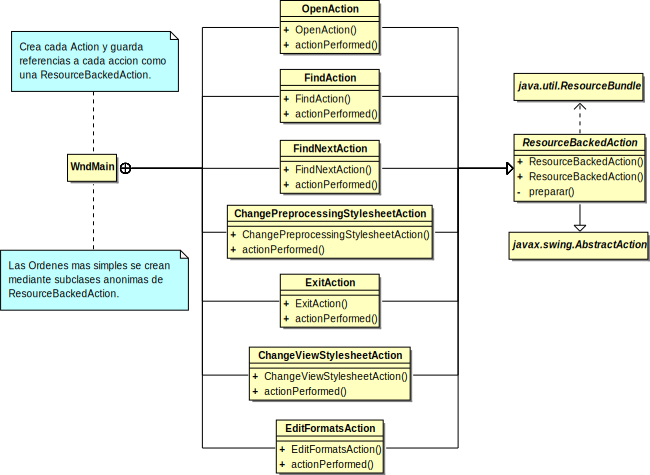
\includegraphics[width=.95\textwidth]{desarrollo/implementacion/clases_localizacion}
  \caption{Diagrama de clases de �rdenes}
  \label{fig:diag_clases_impl_ordenes}
\end{figure}

Tambi�n hay men�s (\clase{ResourceBackedMenu}) y botones
(\clase{ResourceBackedButton}) que extraen sus valores de los
\clase{ResourceBundle}.

\subsection{Hojas XSLT}
\label{sec:cod_xsl}

Las propias hojas \ac{XSLT} deben seguir una serie de convenciones en
su c�digo y forma de operar. Estas convenciones se hallan documentadas
en el apartado del manual de usuario dedicado a explicar c�mo crear
nuevas hojas \ac{XSLT}.

%%% Local Variables: 
%%% mode: latex
%%% TeX-master: "../../memoria"
%%% End: 


\section{Pruebas y validaci�n}
%%
%% Pruebas realizadas
%% Copyright (C) 2008 Antonio Garc�a Dom�nguez
%% $Id: pruebas.tex 635 2008-07-10 23:33:38Z antonio $
%%

Se dar� una breve introducci�n a los conceptos relacionados con las
pruebas de software en \ac{XP} y a continuaci�n se describir� el plan
de pruebas, junto con la especificaci�n de los casos de prueba y su
procedimiento de ejecuci�n.

\subsection{Pruebas en XP}
\label{sec:pruebas_xp}

La metodolog�a \ac{XP} realiza cuatro tipos de pruebas:

\begin{description}
\item[Pruebas de unidad] 
  \index{prueba!unidad} 

  Las pruebas de unidad comprueban de forma autom�tica la
  funcionalidad de un conjunto reducido y cohesivo de clases. Son
  escritas por los propios programadores, siguiendo la pr�ctica de
  \ac{XP} de la programaci�n basada en pruebas.

\item[Pruebas de aceptaci�n] 
  \index{prueba!aceptaci�n}

  Las pruebas de aceptaci�n son escritas
  por el propio cliente con asistencia de los miembros especializados
  en pruebas del equipo de desarrollo.

  M�s que probar el funcionamiento de un par de clases o de un m�todo
  determinado, lo que se intenta probar es la implementaci�n
  satisfactoria de una historia de usuario.

  As�, las pruebas de aceptaci�n suelen describirse mediante una serie
  de pasos en los cuales se utiliza el sistema completo para llevar a
  cabo una tarea. Cada paso tiene un resultado esperado asociado.

\item[Pruebas de integraci�n]
  \index{prueba!integraci�n}

  En \ac{XP}, las pruebas de integraci�n se realizan de forma
  constante. Aunque en mi caso no son importantes al ser un proyecto
  individual, \ac{XP} requiere que todo cambio hecho en una sesi�n de
  programaci�n (en parejas, por supuesto) sea integrado inmediatamente
  en el repositorio central.

  Por supuesto, esto implica que dichas modificaciones deben de haber
  pasado antes por todas las pruebas con �xito, asegur�ndonos de que
  no se han introducido nuevos fallos en otras partes del programa
  inadvertidamente.

\item[Pruebas de implantaci�n] 
  \index{prueba!implantaci�n}

  Una de las pr�cticas recomendadas (que no obligatorias) de \ac{XP}
  es la implantaci�n incremental. Desde el inicio de un proyecto, el
  sistema debe de implantarse en un entorno similar al real,
  posiblemente a menor escala, y comprobarse su correcto
  funcionamiento.

  Estas pruebas, sin embargo, no son especialmente importantes para
  una aplicaci�n de escritorio como la de este proyecto.

\end{description}

\subsection{Plan de pruebas}
\label{sec:pruebas_plan}

\subsubsection{Alcance}

Se determin� que, con las limitaciones de tiempo establecidas, no se
pod�an realizar pruebas de todas y cada una de las partes de \visor{},
\yaxml{} y \postprocesador{}.

Se decidi� implementar pruebas autom�ticas sobre los elementos
fundamentales y utilizar pruebas de aceptaci�n manuales sobre lo
dem�s. En particular, se descartaron aquellas clases cuya
funcionalidad depend�a en su mayor�a de bibliotecas externas, como la
interfaz gr�fica o el controlador de transformaciones \ac{XSLT}.

En un futuro, se espera reemplazar la mayor parte de las pruebas sobre
la interfaz por pruebas autom�ticas, utilizando los nuevos modelos de
presentaci�n. Actualmente ya se ha comenzado esta labor sobre el
di�logo de gesti�n de formatos.

\subsubsection{Tiempo y lugar}

Adem�s del propio uso frecuente de los conversores y \visor{}, mis
directores de proyecto contribuyeron a la ejecuci�n de pruebas de
aceptaci�n de manera informal a lo largo de la ejecuci�n del PFC.

Las pruebas se han realizado en todo momento durante el desarrollo del
PFC (especialmente las automatizadas), siguiendo la pr�ctica ``Flujo''
de \ac{XP}. Al final de cada iteraci�n, se dedic� un tiempo adicional
para la realizaci�n de pruebas de aceptaci�n manuales.

\subsubsection{Naturaleza de las pruebas}

La totalidad de las pruebas usadas son pruebas de caja negra, por ser
f�ciles de mantener a pesar de cambios en la implementaci�n.

\subsection{Dise�o de pruebas}
\label{sec:pruebas_diseno}

A primera vista, se puede determinar que existen cuatro elementos
fundamentales a probar:
\begin{itemize}
\item \postprocesador{}: �procesa correctamente la salida de
  \ac{ACL2}? �Se obtiene un documento que corresponda sin p�rdidas al
  original y que siga el formato de la \ac{DTD}? �Se trata de un
  m�dulo Perl correctamente estructurado y documentado?

\item \yaxml{}: �analiza sin errores los ficheros de entrada? �Realiza
  una conversi�n sin p�rdidas ni modificaciones de la informaci�n del
  fichero fuente \ac{YAML}? Al igual que en el caso anterior, �tiene
  un nivel m�nimo de calidad como m�dulo Perl?

\item El visor \visor{}: �se validan las entradas? �Se reacciona bien
  ante acciones no v�lidas del usuario? �Obtiene el usuario los
  resultados esperados?
\item La integraci�n entre los conversores y \visor{}: �se realiza con
  �xito? �Se capturan y muestran correctamente los fallos?
\end{itemize}

En base a esto, cada parte requiere una combinaci�n determinada de
varios tipos de pruebas:
\begin{description}
\item[\nombrepostprocesador{}] El desarrollo de este conversor se
  halla guiado por los enunciados Lisp y las salidas de \ac{ACL2} que
  ha de procesar. Por lo pronto, resulta natural estructurar las
  pruebas simplemente alrededor de dichos casos.

  Se puede implementar un mecanismo de pruebas de regresi�n usando
  estos enunciados: una vez se haya validado una salida determinada
  como correcta, se puede mantener dicha salida y comparar las salidas
  posteriores con ella, notificando cualquier cambio de inter�s de
  forma autom�tica.

  En un futuro, cuando el alcance del procesador se ampl�e a
  demostraciones de mayor envergadura, se a�adir�n pruebas de unidad
  sobre las clases de mayor importancia.

\item[\nombreyaxml{}] 

  De forma similar al caso anterior, el desarrollo y revisi�n de este
  conversor se apoya sobre una serie de entradas conocidas: cuando
  alguna entrada falla, se a�ade como caso de prueba y se revisa
  \yaxml{} hasta que vuelven a superarse todas las pruebas.

  A diferencia de \postprocesador{}, no necesitamos registrar las
  salidas anteriores ``buenas'' y compararlas con las actuales, sino
  que podemos usar el ciclo \ac{YAML} $\rightarrow$ \ac{XML}
  $\rightarrow$ \ac{YAML} implementado y establecer directamente la
  equivalencia sem�ntica de los dos ficheros \ac{YAML} original y
  final. Este proceso se halla descrito a mayor nivel de detalle
  en~\S\ref{sec:yaxml_equivalencia}
  (p�gina~\pageref{sec:yaxml_equivalencia}).

\item[\nombrevisor{}] 
  Se podr�a dividir \visor{} en tres partes:

  \begin{enumerate}
  \item La interfaz de usuario: Las limitaciones de tiempo, combinadas
    con la dificultad y la escasez en herramientas automatizadas de
    prueba de las interfaces gr�ficas obliga a usar pruebas de
    aceptaci�n manuales por lo pronto. En un futuro cercano, el nuevo
    dise�o de la capa de presentaci�n basado en modelos de
    presentaci�n permitir� automatizar estas pruebas, limit�ndonos a
    enviar notificaciones de gestos a los modelos de presentaci�n.

    Sin embargo, los componentes relacionados con los �rboles \ac{XML}
    son cruciales para la aplicaci�n, y deben de incluir sin falta
    pruebas automatizadas sobre las propiedades que deben cumplir y el
    comportamiento que deben seguir.

  \item Las hojas de usuario: aunque su realizaci�n ser�a t�cnicamente
    factible, las pruebas de unidad de estas hojas no podr�an
    mantenerse estables, puesto que el formato de salida no lo es: al
    ser \ac{XHTML}, est� sujeto a muchos cambios y retoques a lo largo
    del tiempo. Se puede decir lo mismo acerca del paso de
    preprocesado.

  \item La capa de aplicaci�n: esta capa provee los servicios b�sicos
    sobre los que se apoya la capa de presentaci�n. No probaremos
    aquellas partes que �nicamente dependan de la capa de servicios
    t�cnicos, como el funcionamiento de las transformaciones
    \ac{XSLT}, por ejemplo, pero s� los servicios de nivel superior.

    Por ejemplo, habr� que depurar los repositorios de hojas de estilo
    y de descriptores de formatos, la validaci�n de los campos de los
    descriptores de formato, la correspondencia entre rutas XPath y
    nodos de un �rbol \ac{DOM} \ac{XML}, o las extensiones XPath,
    entre otras cosas.
  \end{enumerate}

\item[Integraci�n] 

  La integraci�n es otro aspecto dif�cil de probar autom�ticamente,
  dado que depende en gran medida del entorno empleado por el usuario
  y de la configuraci�n que haya establecido.

  Sin embargo, se presta bien a pruebas de aceptaci�n manuales sobre
  una configuraci�n realizada de antemano. Se habr� de probar que la
  integraci�n reacciona bien a errores de los programas y de su
  invocaci�n, fallando cuando debe y permitiendo una recuperaci�n
  r�pida.

\end{description}

\subsection{Especificaci�n de los casos de prueba}
\label{sec:pruebas_especificacion}

\subsubsection{\nombrepostprocesador{}}
\label{sec:pruebas_postprocesador}

Cada una de las fuentes Lisp y su salida correspondiente a filtrar por
\postprocesador{} seg�n las historias de usuario planteadas es
utilizada como una prueba de regresi�n semiautom�tica.

Describiremos brevemente el contenido de las fuentes Lisp usadas como
casos de prueba. Por claridad, usaremos notaci�n infija. Todos estos
enunciados se encuentran bajo el subdirectorio \fichero{t/testInputs}
de \postprocesador{}.

Durante las pruebas se desactiva todo almacenamiento de resultados
intermedios y se obliga a actualizar el grafo completo de dependencias,
para evitar que en ejecuciones distintas de las pruebas se consigan
resultados distintos.

\begin{itemize}
\item \fichero{triple-rev}

  \fichero{triple-rev} fue el objetivo de la primera iteraci�n. En
  esta demostraci�n se comprueba para una funci�n de inversi�n de
  listas Lisp \evento{rev} que $$rev(rev(rev(x))) = rev(x)$$ para
  toda lista que le pasemos, sea cual sea su estructura.

\item \fichero{equal-app}

  En esta demostraci�n se comprueban ciertas propiedades acerca de las
  funciones \evento{app} para concatenaci�n de listas, \evento{dup}
  para duplicaci�n de cada elemento y \evento{properp} para
  comprobaci�n de listas propias, terminadas mediante \evento{nil},
  como \evento{(a b)} o \evento{(a . (b))} pero no \evento{(a . b)}.

  \begin{itemize}
  \item Asociatividad: $app(app(a,b), c) = app(a, app(b, c))$
  \item Distributividad de la duplicaci�n de cada elemento respecto de
    la concatenaci�n: $app(dup(a),dup(b)) = dup(app(a,b))$
  \item Toda lista a la que se a�ade \lisp{nil} es propia:
    $properp(app(a,nil))$.
  \end{itemize}

\item \fichero{fallo-defun}

  Realmente, este gui�n no trata de probar nada: est� dise�ado para
  ver si \postprocesador{} es capar de tratar los fallos en las
  demostraciones de los \orden{defun}.

  En primer lugar, declaramos una funci�n de c�lculo de factorial
  correcta, que siempre da un resultado correcto y siempre para.

  La siguiente versi�n err�neamente usa $=$ en vez de $zp$, y por lo
  tanto no para nunca para otra cosa que no sea un natural. $zp$ es
  verdadero para toda cosa que no sea un n�mero mayor que cero:
  listas, �tomos, enteros no positivos (incluyendo el cero, claro),
  etc. Sin embargo, $=$ s�lo es verdadero si lo que se pasa es cero,
  por lo que ante un n�mero negativo, por ejemplo, nunca llegar�a al
  caso base y se quedar�a siempre en el caso recursivo.

  En la tercera versi�n, no hay caso base: se ha reemplazado por una
  llamada recursiva a s� mismo. Y en la cuarta y �ltima, no se reduce
  el tama�o de la entrada, imposibilitando tambi�n la parada.

\item \fichero{hanoi}

  No es uno, sino realmente cuatro casos de prueba, al tratarse de un
  proyecto de \ac{ACL2} con tres ficheros Lisp. Tenemos un caso de
  prueba por fichero y otro caso de prueba m�s para la detecci�n del
  grafo que forman y su correcto uso:

  \begin{itemize}
  \item \fichero{hanoi-use.lisp} es el fichero ra�z del
    proyecto. Utiliza la orden \orden{include\hyp{}book} para acceder
    a la definici�n de la funci�n que resuelve el problema de las
    torres de Hanoi, \evento{hanoi::hanoi}, que se halla en el libro
    \libro{books/hanoi}.

  \item \fichero{books/hanoi.acl2} es el fichero Lisp que sirve para
    certificar los contenidos del libro \libro{hanoi} dentro de su mundo
    l�gico inicial. Se podr�a haber llamado \fichero{cert.acl2} si se
    hubiera deseado emplear para cualquier libro dentro de
    \fichero{books}, siguiendo las convenciones usuales de manejo de
    libros de \ac{ACL2}~\cite{ACL2:BookMakefiles}, pero se ha
    preferido esta forma espec�fica, para cuando se a�adan m�s libros
    posteriormente.

  \item \fichero{books/hanoi.lisp} es el propio libro con las
    definiciones necesarias, que asume que se halla dentro del mundo
    l�gico inicial definido por el fichero de certificaci�n
    anterior. Define las funciones \evento{move}, que genera una
    instrucci�n del tipo ``mover un disco de la pila A a la pila B'' y
    \evento{hanoi}, que resuelve el problema de las Torres de Hanoi
    para $n$ discos. Tambi�n incluye un teorema, \evento{len-append},
    que establece que la longitud de la concatenaci�n de dos listas es
    la suma de sus longitudes.

  \end{itemize}

\item \fichero{mapnil}

  En este caso, se demuestra la conmutatividad entre la duplicaci�n de
  los elementos mediante \evento{dup} y la sustituci�n de todo
  elemento de una lista Lisp por \evento{nil} mediante
  \evento{mapnil}.

\item \fichero{memp}

  Dada una funci�n \evento{memp} que comprueba la pertenencia de un
  elemento a una lista y otra funci�n \evento{app} que concatena dos
  listas, se demuestra que $$memp(e, app(a,b)) \equiv memp(e,a) \vee
  memp(e,b),$$ es decir, que todo elemento de la concatenaci�n de las
  dos listas pertenecer� a una u a otra.
  
\item \fichero{miscDefs}

  Comprobamos que \postprocesador{} es capaz de filtrar una
  diversidad de funciones, como b�squedas en diccionarios,
  implementaci�n de aritm�tica mediante el uso de la longitud de las
  listas, recolecci�n de elementos �nicos, potenciaci�n, etc.

  Algunos ejemplos:
  \begin{itemize}
  \item $mapnil(x)$ convierte todos los elementos a \lisp{nil}.
  \item $add(x,y)$ realiza la suma mediante el n�mero de elementos de
  ambas listas. Es decir, implementamos la suma creando una lista de 5
  elementos cuando nos dan una de 2 y otra de 3.
  \item $app(a,b)$ Concatenamos dos listas.
  \item $mem(e,x)$ Devuelve el primer par de la lista tal que el primer
    elemento sea $e$, o $nil$.
  \item $lonesomep(e,lst)$ Comprobamos que $e$ es �nico en la lista.
  \item $collect-lonesomep(a,b)$ Recoge los elementos de la lista $a$ que
    son �nicos en la lista $b$.
  \item $mult(x,y)$ Multiplica a trav�s de longitudes de listas. Si le damos
    una lista con 2 elementos y otra con 3, nos crea una lista con 6.
  \item $fact(n,a)$ Calcula el productorio en aritm�tica sobre
    longitud de listas de las sublistas de la lista que le pasemos.
  \item $fact1(n,a)$ Versi�n recursiva final de \evento{fact}.
  \item $foundp(x,a)$ Busca una clave dentro de un diccionario Lisp. Si el
    diccionario es la lista Lisp de la forma \lisp{((a 2) (b 3))}, sus
    claves son $a$ y $b$.
  \end{itemize}
  
\item \fichero{suma}

  Este caso comprueba que se tratan de forma correcta los
  \evento{defthm} que no requieren inducci�n alguna. Aqu�, \ac{ACL2}
  s�lo tiene que aplicar sus reglas predefinidas sobre la aritm�tica
  decimal para ver que $2 + 2 = 4$ o que $a + b + c = b + c + a$.

  Tambi�n se comprueba que se manejan bien los elementos de listas
  Lisp con la sintaxis \verb!|texto|!.

\item \fichero{swaptree}

  Se define una funci�n \evento{swaptree} que invierte dos �rboles
  Lisp, y se demuestra que es idempotente.

\item \fichero{tail-rev}

  Se define una implementaci�n trivial de la inversi�n de una lista
  \evento{rev} sabiendo que es correcta. Hecho eso, definimos una
  implementaci�n recursiva final obtenida por la transformaci�n
  mediante desplegado-plegado \evento{rev1}. Ahora comprobamos que
  est� bien hecha, es decir, que da los mismos resultados que la
  versi�n original.

\item \fichero{treecopy}

  Es parecida a \evento{swaptree}, pero en este caso lo que se hace es
  copiar un �rbol Lisp, y comprobar que dicha funci�n repite siempre
  la entrada que se le suministra.

\item \fichero{triple-rev-misspell}

  Este caso de prueba es una modificaci�n de \fichero{triple-rev} con
  un fallo en el nombre de un par�metro formal introducido
  intencionadamente, que origina una demostraci�n fallida de la
  longitud suficiente como para ser de inter�s. Adem�s, permite
  comprobar que se tratan bien los errores de \evento{defthm}.

\item \fichero{tutorialWebACL2}

  Este otro caso de prueba es el proyecto de un solo fichero m�s
  completo de todos. En este caso, se desea probar que un algoritmo
  para la inversi�n de una lista Lisp que s�lo hace uso de las
  funciones predefinidas \lisp{endp} (predicado para detectar el
  final de una lista), \lisp{cons} (creaci�n de un par Lisp),
  \lisp{car} (extracci�n de la cabecera) y \lisp{cdr} (extracci�n
  de la cola) es equivalente al algoritmo trivial.

  El proceso es algo m�s complicado que los ejemplos anteriores, y
  puede verse en~\cite{jsmweb}, donde se usa ``El M�todo'',
  acumul�ndose teoremas a demostrar en forma de una pila, donde un
  teorema puede requerir para su demostraci�n verificar otros teoremas
  o lemas.

  Se hacen uso de algunos elementos m�s avanzados, como \orden{thm},
  que lanza una demostraci�n pero no guarda sus resultados en el mundo
  l�gico de \ac{ACL2}, \orden{local} que evita que las reglas
  generadas por un evento sean accesibles fuera de un
  \orden{encapsulate} o libro, y \orden{encapsulate}, que permite
  realizar demostraciones controlando qu� reglas se producen y cu�l es
  la signatura de las funciones definidas.

\end{itemize}

Las pruebas de regresi�n comparan los �rboles \ac{XML} de los
resultados esperados con los obtenidos, empleando el m�dulo
\modulo{XML::SemanticDiff}. Las diferencias detectadas son filtradas
por un predicado que determinan si constituyen una regresi�n o
no. Actualmente, algunas de las diferencias ignoradas son:

\begin{itemize}
\item Cambios en los tiempos de ejecuci�n.
\item Cambios en la versi�n de \ac{ACL2}.
\item Cambios de may�sculas y min�sculas y barras en nombres de
  fichero en Windows.
\item Mensajes de compilaci�n durante la certificaci�n de un libro
  (dependen del compilador y sistema operativo usado).
\end{itemize}

Las pruebas de regresi�n no son las �nicas realizadas. Integradas
dentro del marco de pruebas creado por el m�dulo
\modulo{ExtUtils::MakeMaker} se hallan tambi�n algunas pruebas de
car�cter m�s general:

\begin{itemize}
\item El m�dulo principal debe de poder cargarse con �xito. Esto nos
  asegura de que no nos hayamos olvidado de instalar o referenciar a
  alg�n m�dulo importante en nuestro c�digo.

\item Se debe de haber retirado el texto in�til de las plantillas
  inicialmente generadas por \verb#h2xs#, la herramienta ocupada de
  crear el esqueleto b�sico de todo m�dulo Perl.

\item Todos los ficheros fuente del m�dulo Perl han de incluir el
  aviso de la licencia \ac{GPL}.
\end{itemize}

\subsubsection{\nombreyaxml{}}
\label{sec:pruebas_yaxml}

Como otro m�dulo Perl m�s, \yaxml{} emplea el mismo marco de pruebas y
las pruebas de car�cter general de \postprocesador{}. Este m�dulo usa
tambi�n pruebas de regresi�n, pero son completamente autom�ticas en
este caso, como ya se explic� anteriormente. Ciertas pruebas de
regresi�n son m�s bien para la versi�n refinada de \ac{YAXML}
implementada para cerrar el ciclo \ac{YAML} $\rightarrow$ \ac{XML}
$\rightarrow$ \ac{YAML} que para \yaxml{} en s�.

Algunos casos de prueba se corresponden con documentos reales usados
por herramientas conocidas, y algunos s�lo depuran ciertos aspectos
esenciales. Existe cierto solapamiento entre ambos tipos. Los ficheros
\fichero{.yaml} utilizados como casos de prueba son:

\begin{itemize}
\item \fichero{djangoJSON}

  Este es un ejemplo de un volcado de una base de datos realizado por
  el entorno de desarrollo de aplicaciones Web Django
  (\url{http://www.djangoproject.com/}). Tiene la particularidad de
  usar \ac{JSON}, un subconjunto de \ac{YAML} 1.1, motivando el cambio
  del m�dulo \modulo{YAML::Syck} a \modulo{YAML::XS}.

  % JSON: YAML 1.1

\item \fichero{djangoJSON\_blockIndicatorTest}

  % Indicador de texto

  Otro volcado de Django en el cual se hace patente la necesidad en
  \ac{YAXML} de tener cuidado con el espaciado en blanco y no
  cambiarlo inadvertidamente. En particular, hay que tener cuidado con
  el �ltimo salto de l�nea final, evitando introducirlo cuando
  originalmente no estaba, utilizando el indicador ``|-'' en el estilo
  de bloque para escalares.

\item \fichero{firefoxBookmarks}

  % Ejemplo del "mundo real", JSON, UTF-8

  Una copia de seguridad de los marcadores de Firefox 3 realizada
  tambi�n en \ac{JSON}, que en este caso ten�a la complicaci�n de
  emplear caracteres de \ac{UTF}-8, en particular ideogramas
  japoneses. Se identificaron y resolvieron diversas cuestiones
  relacionadas gracias a este ejemplo.

\item \fichero{fiveMinutes1}

  % Soporte b�sico

  Es uno de los casos m�s b�sicos: un flujo de 4 documentos que
  emplean secuencias de \ac{YAML}. Es compatible con \ac{YAML} 1.0 en
  adelante, al igual que todos los casos de prueba que vienen a
  continuaci�n.

\item \fichero{fiveMinutes2}

  % Claves que no son valores v�lidos en XML

  Este ejemplo muestra ejemplos de vectores asociativos de \ac{YAML}
  1.0, y fue el primer caso de prueba que mostraba la necesidad de
  rodear las limitaciones de \ac{XML} respecto a los identificadores
  v�lidos para una etiqueta utilizando los elementos \verb#_key# y
  \verb#_value#.

\item \fichero{fiveMinutes3}

  % Claves que requieren cuidado especial al devolverlas a YAML

  Desarrollando sobre el ejemplo anterior, este caso de prueba tambi�n
  usa claves de vectores asociativos no directamente representables en
  \ac{XML}, pero adem�s una de ellas requiere un especial cuidado a
  devolverla a \ac{YAML}, o producir�a un error de sintaxis, al
  contener la secuencia ``: ''.

\item \fichero{fiveMinutes4}

  % Estilos de bloques escalares

  Este caso de prueba utiliza los estilos literal y de l�neas reunidas
  para los escalares. En el estilo literal el espaciado no es
  modificado excepto por el indentado de cada l�nea. En el estilo de
  l�neas reunidas, todas las palabras separadas por �nicamente un
  car�cter de espaciado (como un espacio o un salto de l�nea) son
  reunidas en una sola l�nea.

\item \fichero{fiveMinutes5}

  % Estilos de bloque y flujo de colecciones

  El �ltimo ejemplo de la serie~\cite{YamlInFiveMinutes} ilustra c�mo
  pueden escribirse tambi�n las colecciones con distintos estilos, ya
  sea de bloque, con un elemento por l�nea, o de flujo, que permite
  definir m�s de un elemento en cada l�nea.

\item \fichero{invoice}

  % Manejo de anclas y alias (mapa anclado)
  % YAML complejo

  Este caso de prueba es uno de los ejemplos incluidos en la
  especificaci�n \ac{YAML}~\cite{YAML}, y precisamente el que ilustra
  el uso de anclas y alias para evitar tener que repetir el contenido
  com�n a dos nodos.

\item \fichero{mappingAnchoredSequence}

  % Manejo de anclas y alias (secuencia anclada)

  Aqu� probamos a transformar un documento en que el documento anclado
  no es un mapa, sino una secuencia.

\item \fichero{podExample}

  % Depura el ejemplo del POD de YAXML::Reverse

  Este ejemplo tan sencillo es el usado en la documentaci�n \ac{POD}
  de \yaxml{}, para poder garantizar que funcione.

\item \fichero{yaxmlReverseMETA}

  % YAML del "mundo real"
  
  Se trata del fichero \fichero{META.yaml} de \yaxml{}. Estos ficheros
  son utilizado por diversas herramientas autom�ticas, como las que
  utiliza el CPAN, para obtener informaci�n de autor�a y dependencias.

\end{itemize}

\subsubsection{Visor e integraci�n}
\label{sec:pruebas_visor}

\paragraph{Pruebas de unidad}
\label{sec:pruebas_visor_unidad}

Las pruebas de unidad definidas para cada clase comprueban una serie
de propiedades acerca de su comportamiento. En lugar de dar una
especificaci�n exacta de cada prueba (que s�lo ser�a repetir el
c�digo), listaremos las propiedades que verifican.

Estas pruebas, basadas en el marco JUnit, se ejecutan de forma
autom�tica y son un objetivo m�s dentro del fichero de tareas Ant.

Toda clase de pruebas tiene el nombre formado por el nombre de la
clase cuyo funcionamiento comprueba y a continuaci�n el sufijo
``Test''.

\begin{description}
\item[\clase{CommandBuilderTest}] 

  Se comprueba que se realiza la sustituci�n de las claves y la
  divisi�n en argumentos correctamente, independientemente de que los
  argumentos contengan espacios, mientras tengan comillas alrededor de
  la orden original.

\item[\clase{DataDrivenTreeModelTest}] 

  Todo nodo del documento \ac{XML} oculto mediante el atributo
  correspondiente debe ser inaccesible a trav�s de un recorrido
  exhaustivo.

  Adem�s, el modelo ha de informar de que todo nodo con el atributo
  requerido para la falsa poda activado no tiene hijos, y �stos deben
  ser completamente inaccesibles desde dicho modelo.

\item[\clase{DOMTreeModelTest}] 

  El modelo ofrecido por dicha clase debe de ser el mismo que ofrece
  el �rbol \ac{DOM} original del documento, limit�ndose a los nodos
  de tipo elemento.

\item[\clase{DOMTreeTest}] 

  Debe de poderse realizar una navegaci�n completa a trav�s del �rbol,
  ignorando toda petici�n no v�lida, como intentar ir al padre de la
  ra�z.

\item[\clase{ExtensionFileFilterTest}] 

  Se prueba que se a�ade autom�ticamente la extensi�n al nombre de
  fichero si no est� presente, que se conserva si ya est�, y que se
  conserva el nombre de fichero si no se usa un filtro
  \clase{FiltroExtensi�n}.

\item[\clase{FormatDescriptorRepositoryTest}] 

  Utilizando un repositorio a dos niveles con el descriptor de formato
  \fichero{xml.format} incluido con \visor{}, se comprueba que se
  inicializa correctamente. Tambi�n se prueba a cambiar un descriptor,
  guardarlo y volver a cargar, para ver si los cambios se han
  realizado.

  A continuaci�n se hacen pruebas sobre la capacidad de localizar las
  cadenas de un descriptor de formato, de que los cambios realizados a
  un descriptor vayan al repositorio de mayor prioridad, y que se
  puedan restaurar las opciones originales de un formato.

  Finalmente, se comprueba que los mutadores de todo descriptor de
  formato lancen ciertas excepciones al pasarles alg�n valor
  no v�lido.

\item[\clase{SerializedPreferencesManagerTest}] 

  Se comprueba que se puede crear un fichero de preferencias nuevo, y
  que inicialmente est� vac�o. Debe adem�s poder guardar de forma
  persistente escalares y listas.

\item[\clase{StylesheetRepositoryTest}] 

  Se verifica que las hojas incluidas en \visor{} pueden localizarse
  sin problemas dentro del repositorio, que se hallan debidamente
  configuradas y que su c�digo \ac{XSLT} compila sin problemas.

\item[\clase{VectorNodeListTest}] 

  Se prueba que el m�todo \metodo{invertir} realmente cumple su tarea,
  y que la inversi�n es idempotente.

\item[\clase{WndFormatsPresentationModelTest}] 

  Se comprueba que cuando el usuario seleccione un elemento, cambie el
  nombre y confirme los cambios estos se realicen de forma correcta y
  persistente.

\item[\clase{XHTMLSearchKeyHighlighterTest}] 

  Al destacar una clave dentro de un documento \ac{XHTML} los
  elementos \ac{XHTML} deben de conservarse intactos. No debe
  modificarse otra cosa que el contenido del documento en s�, es
  decir, el fragmento situado dentro del elemento \verb|body|.

  Deben adem�s de manejarse bien los casos en que la clave a marcar
  est� justo antes o despu�s de un elemento \ac{XHTML}. Otros casos
  importantes a tratar incluyen el manejo correcto de marcado de s�lo
  palabras completas o sin tener en cuenta may�sculas y min�sculas.

\item[\clase{XPathExtensionsTest}] 

  Se comprueba que se obtienen coincidencias de la forma esperada para
  varias combinaciones posibles de tipos de clave y cadena de
  b�squeda.

  As�, la clave de b�squeda podr�a componerse s�lo de caracteres
  alfanum�ricos. Tambi�n podr�a contener espacios o caracteres no
  alfanum�ricos. Se podr�a dar el caso de que el usuario introdujera
  alg�n car�cter que deber�a escaparse para no ser interpretado como
  un metacar�cter en una expresi�n regular.

  El texto en el que buscar podr�a contener espacios iniciales o
  finales, o saltos de l�nea.

  Tambi�n podr�a darse el caso en que la clave y el texto fueran
  iguales, o que alguno de los dos estuviera vac�o.

\item[\clase{XPathPathManagerTest}] 

  Se comprueba que la ruta XPath generada de cualquier nodo del �rbol
  \ac{DOM} de un determinado documento \ac{XML} es correcta, y que la
  obtenci�n de un nodo a partir de su ruta XPath se realiza tambi�n
  con �xito.
  
\end{description}

\paragraph{Pruebas de aceptaci�n}
\label{sec:pruebas_visor_acept}

Pasaremos a establecer una prueba de aceptaci�n para cada una de las
historias de usuario acumuladas desde las primeras versiones de
\visor{} hasta ahora. Dichas pruebas se ejecutan de forma manual.

\begin{itemize}
\item

  \begin{quote}
    ``Visualizar un documento \ac{XML} arbitrario en forma de �rbol,
    permitiendo expandir y contraer los nodos y buscar informaci�n.''
  \end{quote}

  Cuadro~\ref{acept:visualizarxml}, p�gina~\pageref{acept:visualizarxml}.

  \begin{table}[tbp]
    \centering
    \begin{pruebaaceptacion}
      El usuario solicita la apertura de un fichero. & Se muestra el
      di�logo de elecci�n de ficheros. \\ \hline

      El usuario elige un fichero \ac{XML}. & Tras la compilaci�n de las
      hojas y el preprocesado, se muestra el primer nodo del documento. \\ \hline

      El usuario cambia la hoja de preprocesado a \verb|xml|. & El �rbol
      del documento muestra el �rbol \ac{XML} original. \\ \hline

      El usuario cambia la hoja de visualizaci�n a \verb|xml|. & La
      visualizaci�n muestra todos los atributos, ancestros e hijos. \\ \hline

      El usuario cambia la hoja de visualizaci�n a \verb|xmlSource|. &
      La visualizaci�n muestra el c�digo \ac{XML} completo de cada
      nodo seleccionado tras su preprocesado. \\ \hline

      El usuario navega por el �rbol, usando cada una de las opciones
      disponibles de navegaci�n [...] & La visualizaci�n se actualiza en
      cada cambio de nodo, mostrando la informaci�n correcta. \\ \hline

      El usuario solicita expandir el �rbol. & El �rbol del documento se
      expande en su totalidad. \\ \hline

      El usuario solicita contraer el �rbol. & El �rbol del documento
      se contrae, y se muestra solamente el primer nodo del
      documento. \\ \hline

      El usuario realiza una b�squeda de una clave existente en el
      documento. & Se muestra el primer resultado, con el marcado de la
      clave de b�squeda en la visualizaci�n. \\ \hline

      El usuario pulsa de nuevo en el bot�n de Buscar del di�logo o
      utiliza el elemento del men� Navegar ``Buscar Siguiente''. & Se
      muestran el resto de los resultados. \\ \hline

      El usuario lanza de nuevo la b�squeda al llegar al �ltimo
      resultado. & Se muestra de nuevo el primer resultado. \\ \hline

      El usuario prueba con el resto de las opciones de filtrado en
      secuencia y compara con los resultados anteriores [...] & Se
      comprueba el filtrado del conjunto de resultados obtenido
      anteriormente. \\ \hline
    \end{pruebaaceptacion}
    \caption{Prueba de aceptaci�n para ``Visualizar XML gen�rico''}
    \label{acept:visualizarxml}
  \end{table}

\item 
  \begin{quote}
    ``El visor no deber�a saber absolutamente nada de \ac{ACL2}. Nada
    en su interfaz gr�fica ni en su implementaci�n nos debe recordar
    que podemos trabajar con \ac{ACL2}.''
  \end{quote}

  Cuadro~\ref{acept:indepacl2}, p�gina~\pageref{acept:indepacl2}. Se
  asume en esta historia que \visor{} ha sido instalado desde cero,
  sin ning�n otro a�adido.

  \begin{table}
    \centering
    \begin{pruebaaceptacion}
      El usuario abre \visor{}. & Se muestra la ventana principal. \\
      \hline

      El usuario abre un documento \ac{XML} cualquiera. & Se muestra
      su primer nodo. \\ \hline

      El usuario comprueba la lista de hojas de preprocesado
      disponibles. & S�lo se dispone de la hoja \verb#xml#. \\ \hline

      El usuario comprueba la lista de hojas de visualizaci�n
      disponibles. & S�lo se dispone de las hojas \verb#xml# y
      \verb#xmlSource#. \\ \hline

      El usuario intenta abrir otro documento, y prueba a desplegar el
      filtro de tipos de documento. & S�lo se dispone de las
      opciones ``Todos los ficheros'' o ``Fichero XML normal''. \\
      \hline

      El usuario cancela su acci�n y abre el di�logo de gesti�n de
      formatos. & Se muestra el di�logo con un �nico formato:
      ``Fichero XML normal''. \\ \hline
      
    \end{pruebaaceptacion}
    \caption{Prueba de aceptaci�n para ``Hacer a \visor{} independiente de \acs{ACL2}''}
    \label{acept:indepacl2}
  \end{table}

\item 
  \begin{quote}
    ``A�adir soporte para visualizar varios ficheros a la vez y
    enlazarlos entre s�.''
  \end{quote}

  Cuadro~\ref{acept:multidoc}, p�gina~\pageref{acept:multidoc}. Se
  asume que se ha instalado \ac{ACL2}, \postprocesador{}, sus hojas de
  usuario y su descriptor de formato de la manera descrita en el
  manual de usuario.

  \begin{table}
    \centering
    \begin{pruebaaceptacion}
      El usuario abre un documento \ac{XML} cualquiera. & Se muestra
      su primer nodo. \\ \hline

      El usuario cambia las hojas de visualizaci�n y preprocesado a
      las hojas b�sicas \verb#xml#. & Se muestra el documento \ac{XML}
      tal y como est�, listando en cada nodo sus atributos y dando las
      cabeceras y pies apropiados. \\ \hline

      El usuario abre el caso de prueba \fichero{hanoi-use.lisp} de
      \postprocesador{}. & Se muestra su primer nodo en una pesta�a
      aparte, con las mismas hojas que en la primera pesta�a. \\
      \hline

      El usuario cambia las hojas de visualizaci�n y preprocesado a
      las hojas \verb#ppACL2#. & Se muestran las �rdenes
      \orden{include-book} y \orden{defthm} que conforman al
      fichero. \\ \hline

      El usuario selecciona el sumario del \orden{defthm}. & Aparecen
      enlaces a \evento{HANOI::HANOI} entre las reglas usadas. \\ \hline

      El usuario activa el enlace a \evento{HANOI::HANOI}. & Se abre
      \fichero{hanoi.acl2} en una pesta�a, con el nodo en cuesti�n
      seleccionado. \\ \hline

      El usuario vuelve a \fichero{hanoi-use.lisp}, y esta vez activa
      \evento{HANOI::MOVE}. & Se cambia de nuevo a la pesta�a de
      \fichero{hanoi.acl2}, movi�ndose al nodo seleccionado. \\ \hline

      El usuario cambia a la pesta�a del documento \ac{XML}. & El
      documento mantiene la selecci�n anterior y utiliza las hojas de
      preprocesado y visualizaci�n \verb#xml#. \\ \hline
      
    \end{pruebaaceptacion}
    \caption{Prueba de aceptaci�n para ``Visualizar y enlazar varios documentos entre s�.''}
    \label{acept:multidoc}
  \end{table}

\item 
  \begin{quote}
    ``Proporcionar una lista de documentos recientes.''
  \end{quote}

  Cuadro~\ref{acept:recentdocs}, p�gina~\pageref{acept:recentdocs}.

  \begin{table}[tbp]
    \begin{pruebaaceptacion}
      El usuario abre un documento \ac{XML} no presente a�n en el
      historial. & Se muestra dicho documento y aparece su
      entrada en el historial. \\ \hline
      
      El usuario cierra \visor{}. &
      Se guarda el historial de documentos recientes. \\ \hline
      
      El usuario vuelve a ejecutar el programa y examina el historial. &
      Se sigue mostrando entre sus entradas el anterior fichero
      abierto. \\ \hline

      El usuario selecciona dicha entrada. & Se abre de nuevo el
      documento. \\ \hline

      El usuario cierra \visor{}, cambia al documento de localizaci�n y
      vuelve a ejecutar \visor{}. & Se sigue listando al fichero
      en su historial. \\ \hline

      El usuario selecciona la entrada anterior. & Se informa
      que el fichero no existe y elimina la entrada del historial. \\ \hline
    \end{pruebaaceptacion}
    \caption{Prueba de aceptaci�n para ``Historial de documentos recientes''}
    \label{acept:recentdocs}
  \end{table}

\item 
  \begin{quote}
    ``Integrar el visor y el editor preferido del usuario.''
  \end{quote}
  
  Cuadro~\ref{acept:integraredit},
  p�gina~\pageref{acept:integraredit}.

  \begin{table}[tbp]
    \centering
    \begin{pruebaaceptacion}
      El usuario abre un documento \ac{XML} gen�rico. & El sistema
      muestra dicho documento seg�n las hojas actuales. \\ \hline

      El usuario solicita abrir el di�logo de gesti�n de formatos
      admitidos. & Se abre el di�logo de gesti�n de formatos
      admitidos, incluyendo al menos al elemento ``Fichero XML
      normal''. No se puede acceder al formulario principal. \\ \hline

      El usuario comprueba el editor establecido y cierra el
      di�logo. & Se cierra el di�logo, volviendo a poder acceder al
      formulario principal. \\ \hline

      El usuario solicita la edici�n del documento. & Se lanza el
      editor que antes estaba especificado sobre el fichero actual.
      La interfaz gr�fica puede seguir us�ndose en paralelo sin
      problemas. \\ \hline

      El usuario cierra el editor, utiliza el di�logo de formatos
      admitidos para cambiar la orden a otro editor existente en el
      sistema y confirma sus cambios. & Los cambios son guardados. \\
      \hline

      El usuario solicita de nuevo la edici�n del documento. & Se
      lanza el editor especificado anteriormente, y la interfaz
      gr�fica se puede seguir usando sin problemas. \\ \hline

    \end{pruebaaceptacion}
    \caption{Prueba de aceptaci�n para ``Integrar editor''}
    \label{acept:integraredit}
  \end{table}

\item 
  \begin{quote}
    ``Vigilar directamente el fichero fuente en caso de cambios, en vez de
    solamente cuando se cierra el editor. As�, si uno abre el editor, hace
    un par de cambios y guarda (sin cerrar el editor), tambi�n se
    actualizar�. En caso de que se desactive temporalmente la
    reimportaci�n autom�tica, tambi�n deber�a funcionar correctamente si
    en ese intervalo se hicieron cambios.''
  \end{quote}

  Cuadro~\ref{acept:autoactualizar},
  p�gina~\pageref{acept:autoactualizar}.

  \begin{table}[tbp]
    \centering
    \begin{pruebaaceptacion}
      El usuario abre un documento \ac{XML} cualquiera. & El
      sistema muestra dicho documento seg�n las hojas actuales. \\
      \hline

      El usuario solicita la edici�n del documento. & Se abre el
      editor registrado por el usuario para el formato empleado. \\ \hline

      El usuario activa la actualizaci�n autom�tica en las
      preferencias. & La entrada del men� pasa a estar marcada como
      activa. \\ \hline

      El usuario cambia el contenido del documento, manteniendo su
      correcci�n sint�ctica, y guarda los cambios. & El documento se
      vuelve a abrir, y los cambios se reflejan en �l. \\ \hline

      El usuario desactiva la actualizaci�n autom�tica en las
      preferencias. & La entrada del men� pasa a estar marcada como
      inactiva. \\ \hline

      El usuario deshace el cambio anterior, y guarda los cambios. &
      El documento no se reabre. \\ \hline

      El usuario activa de nuevo la actualizaci�n autom�tica en las
      preferencias. & La entrada del men� vuelve a aparecer como
      activa y el documento se reabre, reflejando los cambios
      realizados. \\ \hline

      El usuario hace cambios que violan la correcci�n sint�ctica de
      la entrada. & El proceso de an�lisis sint�ctico falla,
      notific�ndose al usuario del hecho, y por lo dem�s operando de
      forma normal. La copia antigua del documento sigue abierta y
      funciona sin problemas. \\ \hline

    \end{pruebaaceptacion}
    \caption{Prueba de aceptaci�n para ``Actualizar autom�ticamente''}
    \label{acept:autoactualizar}
  \end{table}

\item 
  \begin{quote}
    ``Guardar las preferencias autom�ticamente al cerrar el programa.''
  \end{quote}

  Cuadro~\ref{acept:saveprefs}, p�gina~\pageref{acept:saveprefs}.

  \begin{table}[tbp]
    \centering
    \begin{pruebaaceptacion}
      El usuario, tras abrir un documento \ac{XML}, cambia la hoja de
      preprocesado a un valor distinto. & Se actualiza el documento
      seg�n la nueva hoja. \\ \hline

      El usuario cierra \visor{}. & Se guarda las
      preferencias. \\ \hline 

      El usuario ejecuta de nuevo \visor{}, y abre un documento
      \ac{XML}. & Se conserva la selecci�n de hoja de preprocesado de
      la ejecuci�n anterior. \\ \hline
    \end{pruebaaceptacion}
    \caption{Prueba de aceptaci�n para ``Guardar preferencias''}
    \label{acept:saveprefs}
  \end{table}

\item 
  \begin{quote}
    ``Visualizar un fichero Lisp integrando \visor{} con \postprocesador{}.''
  \end{quote}

  Cuadro~\ref{acept:visualizarxmlpp},
  p�gina~\pageref{acept:visualizarxmlpp}. Se asume que se ha instalado
  \ac{ACL2}, \postprocesador{}, sus hojas de usuario y su descriptor de
  formato de la manera descrita en el manual de usuario.

  \begin{table}[tbp]
    \centering
    \begin{pruebaaceptacion}
      El usuario abre el caso de prueba
      \fichero{triple\hyp{}rev\hyp{}misspell.lisp} de \postprocesador{}. & El
      sistema muestra el primer nodo del documento. \\ \hline

      El usuario selecciona la hoja de preprocesado
      \fichero{ppACL2}. & Se actualiza el documento y muestra
      el �rbol debidamente decorado con los nombres de los eventos y
      los iconos de �xito y fracaso, seleccionando y mostrando el
      primer nodo de la visualizaci�n. En particular, deber�a de haber
      un �nico elemento marcado como fracaso: \evento{REV-REV}, hijo
      directo del nodo ra�z. \\ \hline

      El usuario selecciona la hoja de visualizaci�n
      \fichero{ppACL2}. & Se actualiza la visualizaci�n del
      nodo actual, pasando a mostrar solamente la informaci�n
      relacionada con \ac{ACL2}: los nombres de cada evento y el
      c�digo Lisp asociado.  \\ \hline

      El usuario navega por el �rbol del documento [...] & Se
      visualiza la informaci�n correspondiente al nodo de la forma
      esperada. En particular, deber�a de informar del punto exacto
      del fracaso de \evento{REV-REV} a trav�s de una cadena de iconos
      de fracaso. \\ \hline
    \end{pruebaaceptacion}
    \caption{Prueba de aceptaci�n para ``Integrar \visor{} y \postprocesador{}''}
    \label{acept:visualizarxmlpp}
  \end{table}

\item 
  \begin{quote}
    ``Implementar la hoja \fichero{summaries}, que pode el �rbol y deje
    solamente los res�menes, y la hoja \fichero{reverse}, que invierta
    el orden de los eventos, para mostrar primero las conclusiones y
    luego sus antecedentes.''
  \end{quote}

  Cuadro~\ref{acept:summaryrev}, p�gina~\pageref{acept:summaryrev}. Se
  asume que se ha instalado \postprocesador{}, su descriptor de
  formato y sus hojas de usuario tal y como se describe en el manual
  de usuario.

  \begin{table}[tbp]
    \centering
    \begin{pruebaaceptacion}
      El usuario abre un documento Lisp. & El
      sistema muestra el primer nodo del documento. \\ \hline
      El usuario selecciona la hoja de visualizaci�n \fichero{ppACL2}. & El
      sistema actualiza el nodo seleccionado. \\ \hline
      El usuario selecciona la hoja de preprocesado \fichero{summaries}. & El
      sistema actualiza el documento, que ahora s�lo muestra las �rdenes
      y los sumarios. \\ \hline
      El usuario selecciona la hoja de preprocesado \fichero{reverse}. & El
      sistema actualiza el documento, en el que los eventos se hallan en
      orden inverso al que siguen en la fuente Lisp. \\ \hline
    \end{pruebaaceptacion}
    \caption{Prueba de aceptaci�n para ``Hojas \fichero{summary} y \fichero{reverse}''}
    \label{acept:summaryrev}
  \end{table}

\item 
  \begin{quote}
    ``A�adir informaci�n acerca del uso de una meta, como sus
    dependencias inversas.''
  \end{quote}

  Cuadro~\ref{acept:usometa}, p�gina~\pageref{acept:usometa}. Se asume
  que \postprocesador{} se halla debidamente instalado.

  \begin{table}[tbp]
    \centering
    \begin{pruebaaceptacion}
      El usuario abre un documento Lisp. & El
      sistema muestra el primer nodo de dicho documento seg�n las
      hojas actuales. \\ \hline

      El usuario selecciona la hoja de preprocesado \fichero{ppACL2} y
      la hoja de visualizaci�n \fichero{ppACL2}. & Se actualiza
      el documento y la visualizaci�n, ahora estructurados ambos en
      �rdenes y demostraciones de \ac{ACL2}. \\ \hline

      El usuario selecciona el primer evento usado por otros
      eventos. & Se muestra dicho nodo, con una lista de enlaces a los
      eventos que lo mencionan. \\
      \hline
    \end{pruebaaceptacion}
    \caption{Prueba de aceptaci�n para ``Ver usos de una meta''}
    \label{acept:usometa}
  \end{table}

\item 
  \begin{quote}
    ``Abrir documentos \ac{YAML} en \nombrevisor{} sin que suponga una
    p�rdida o alteraci�n de la informaci�n disponible.''
  \end{quote}

  Cuadro~\ref{acept:integraryaxml},
  p�gina~\pageref{acept:integraryaxml}. Se asume que se ha instalado
  \yaxml{} con su descriptor de formato y hojas de usuario debidamente.

  \begin{table}
    \centering
    \begin{pruebaaceptacion}
      El usuario abre el caso de prueba \fichero{invoice.yaml} de
      \yaxml{}. & Se muestra su primer nodo. \\ \hline

      El usuario cambia a las hojas de preprocesado y visualizaci�n
      \verb#yaxml#. & Se muestra un �rbol con un �nico documento
      an�nimo, que contiene los mismos elementos que el documento
      \ac{YAML} original. \\ \hline

      El usuario selecciona el elemento \fichero{bill-to} del
      documento. & Se muestran los atributos del elemento, apareciendo
      un enlace en el atributo \verb#yaml:alias#. \\ \hline

      El usuario activa el enlace. & Se selecciona el elemento
      \verb#ship-to# del documento al que hace referencia el ancla. \\
      \hline
      
    \end{pruebaaceptacion}
    \caption{Prueba de aceptaci�n para ``Integrar \visor{} y \yaxml{}''}
    \label{acept:integraryaxml}
  \end{table}

\end{itemize}

%%% Local Variables: 
%%% mode: latex
%%% TeX-master: "../../memoria"
%%% End: 


%%% Local Variables: 
%%% mode: latex
%%% TeX-master: "../memoria"
%%% End: 
